% Options for packages loaded elsewhere
\PassOptionsToPackage{unicode}{hyperref}
\PassOptionsToPackage{hyphens}{url}
\PassOptionsToPackage{dvipsnames,svgnames,x11names}{xcolor}
%
\documentclass[
  letterpaper,
  DIV=11,
  numbers=noendperiod]{scrartcl}

\usepackage{amsmath,amssymb}
\usepackage{iftex}
\ifPDFTeX
  \usepackage[T1]{fontenc}
  \usepackage[utf8]{inputenc}
  \usepackage{textcomp} % provide euro and other symbols
\else % if luatex or xetex
  \usepackage{unicode-math}
  \defaultfontfeatures{Scale=MatchLowercase}
  \defaultfontfeatures[\rmfamily]{Ligatures=TeX,Scale=1}
\fi
\usepackage{lmodern}
\ifPDFTeX\else  
    % xetex/luatex font selection
\fi
% Use upquote if available, for straight quotes in verbatim environments
\IfFileExists{upquote.sty}{\usepackage{upquote}}{}
\IfFileExists{microtype.sty}{% use microtype if available
  \usepackage[]{microtype}
  \UseMicrotypeSet[protrusion]{basicmath} % disable protrusion for tt fonts
}{}
\makeatletter
\@ifundefined{KOMAClassName}{% if non-KOMA class
  \IfFileExists{parskip.sty}{%
    \usepackage{parskip}
  }{% else
    \setlength{\parindent}{0pt}
    \setlength{\parskip}{6pt plus 2pt minus 1pt}}
}{% if KOMA class
  \KOMAoptions{parskip=half}}
\makeatother
\usepackage{xcolor}
\setlength{\emergencystretch}{3em} % prevent overfull lines
\setcounter{secnumdepth}{5}
% Make \paragraph and \subparagraph free-standing
\ifx\paragraph\undefined\else
  \let\oldparagraph\paragraph
  \renewcommand{\paragraph}[1]{\oldparagraph{#1}\mbox{}}
\fi
\ifx\subparagraph\undefined\else
  \let\oldsubparagraph\subparagraph
  \renewcommand{\subparagraph}[1]{\oldsubparagraph{#1}\mbox{}}
\fi

\usepackage{color}
\usepackage{fancyvrb}
\newcommand{\VerbBar}{|}
\newcommand{\VERB}{\Verb[commandchars=\\\{\}]}
\DefineVerbatimEnvironment{Highlighting}{Verbatim}{commandchars=\\\{\}}
% Add ',fontsize=\small' for more characters per line
\usepackage{framed}
\definecolor{shadecolor}{RGB}{241,243,245}
\newenvironment{Shaded}{\begin{snugshade}}{\end{snugshade}}
\newcommand{\AlertTok}[1]{\textcolor[rgb]{0.68,0.00,0.00}{#1}}
\newcommand{\AnnotationTok}[1]{\textcolor[rgb]{0.37,0.37,0.37}{#1}}
\newcommand{\AttributeTok}[1]{\textcolor[rgb]{0.40,0.45,0.13}{#1}}
\newcommand{\BaseNTok}[1]{\textcolor[rgb]{0.68,0.00,0.00}{#1}}
\newcommand{\BuiltInTok}[1]{\textcolor[rgb]{0.00,0.23,0.31}{#1}}
\newcommand{\CharTok}[1]{\textcolor[rgb]{0.13,0.47,0.30}{#1}}
\newcommand{\CommentTok}[1]{\textcolor[rgb]{0.37,0.37,0.37}{#1}}
\newcommand{\CommentVarTok}[1]{\textcolor[rgb]{0.37,0.37,0.37}{\textit{#1}}}
\newcommand{\ConstantTok}[1]{\textcolor[rgb]{0.56,0.35,0.01}{#1}}
\newcommand{\ControlFlowTok}[1]{\textcolor[rgb]{0.00,0.23,0.31}{#1}}
\newcommand{\DataTypeTok}[1]{\textcolor[rgb]{0.68,0.00,0.00}{#1}}
\newcommand{\DecValTok}[1]{\textcolor[rgb]{0.68,0.00,0.00}{#1}}
\newcommand{\DocumentationTok}[1]{\textcolor[rgb]{0.37,0.37,0.37}{\textit{#1}}}
\newcommand{\ErrorTok}[1]{\textcolor[rgb]{0.68,0.00,0.00}{#1}}
\newcommand{\ExtensionTok}[1]{\textcolor[rgb]{0.00,0.23,0.31}{#1}}
\newcommand{\FloatTok}[1]{\textcolor[rgb]{0.68,0.00,0.00}{#1}}
\newcommand{\FunctionTok}[1]{\textcolor[rgb]{0.28,0.35,0.67}{#1}}
\newcommand{\ImportTok}[1]{\textcolor[rgb]{0.00,0.46,0.62}{#1}}
\newcommand{\InformationTok}[1]{\textcolor[rgb]{0.37,0.37,0.37}{#1}}
\newcommand{\KeywordTok}[1]{\textcolor[rgb]{0.00,0.23,0.31}{#1}}
\newcommand{\NormalTok}[1]{\textcolor[rgb]{0.00,0.23,0.31}{#1}}
\newcommand{\OperatorTok}[1]{\textcolor[rgb]{0.37,0.37,0.37}{#1}}
\newcommand{\OtherTok}[1]{\textcolor[rgb]{0.00,0.23,0.31}{#1}}
\newcommand{\PreprocessorTok}[1]{\textcolor[rgb]{0.68,0.00,0.00}{#1}}
\newcommand{\RegionMarkerTok}[1]{\textcolor[rgb]{0.00,0.23,0.31}{#1}}
\newcommand{\SpecialCharTok}[1]{\textcolor[rgb]{0.37,0.37,0.37}{#1}}
\newcommand{\SpecialStringTok}[1]{\textcolor[rgb]{0.13,0.47,0.30}{#1}}
\newcommand{\StringTok}[1]{\textcolor[rgb]{0.13,0.47,0.30}{#1}}
\newcommand{\VariableTok}[1]{\textcolor[rgb]{0.07,0.07,0.07}{#1}}
\newcommand{\VerbatimStringTok}[1]{\textcolor[rgb]{0.13,0.47,0.30}{#1}}
\newcommand{\WarningTok}[1]{\textcolor[rgb]{0.37,0.37,0.37}{\textit{#1}}}

\providecommand{\tightlist}{%
  \setlength{\itemsep}{0pt}\setlength{\parskip}{0pt}}\usepackage{longtable,booktabs,array}
\usepackage{calc} % for calculating minipage widths
% Correct order of tables after \paragraph or \subparagraph
\usepackage{etoolbox}
\makeatletter
\patchcmd\longtable{\par}{\if@noskipsec\mbox{}\fi\par}{}{}
\makeatother
% Allow footnotes in longtable head/foot
\IfFileExists{footnotehyper.sty}{\usepackage{footnotehyper}}{\usepackage{footnote}}
\makesavenoteenv{longtable}
\usepackage{graphicx}
\makeatletter
\def\maxwidth{\ifdim\Gin@nat@width>\linewidth\linewidth\else\Gin@nat@width\fi}
\def\maxheight{\ifdim\Gin@nat@height>\textheight\textheight\else\Gin@nat@height\fi}
\makeatother
% Scale images if necessary, so that they will not overflow the page
% margins by default, and it is still possible to overwrite the defaults
% using explicit options in \includegraphics[width, height, ...]{}
\setkeys{Gin}{width=\maxwidth,height=\maxheight,keepaspectratio}
% Set default figure placement to htbp
\makeatletter
\def\fps@figure{htbp}
\makeatother

\usepackage{float}
\usepackage{tabularray}
\usepackage[normalem]{ulem}
\usepackage{graphicx}
\UseTblrLibrary{booktabs}
\UseTblrLibrary{siunitx}
\NewTableCommand{\tinytableDefineColor}[3]{\definecolor{#1}{#2}{#3}}
\newcommand{\tinytableTabularrayUnderline}[1]{\underline{#1}}
\newcommand{\tinytableTabularrayStrikeout}[1]{\sout{#1}}
\KOMAoption{captions}{tableheading}
\makeatletter
\@ifpackageloaded{caption}{}{\usepackage{caption}}
\AtBeginDocument{%
\ifdefined\contentsname
  \renewcommand*\contentsname{Table of contents}
\else
  \newcommand\contentsname{Table of contents}
\fi
\ifdefined\listfigurename
  \renewcommand*\listfigurename{List of Figures}
\else
  \newcommand\listfigurename{List of Figures}
\fi
\ifdefined\listtablename
  \renewcommand*\listtablename{List of Tables}
\else
  \newcommand\listtablename{List of Tables}
\fi
\ifdefined\figurename
  \renewcommand*\figurename{Figure}
\else
  \newcommand\figurename{Figure}
\fi
\ifdefined\tablename
  \renewcommand*\tablename{Table}
\else
  \newcommand\tablename{Table}
\fi
}
\@ifpackageloaded{float}{}{\usepackage{float}}
\floatstyle{ruled}
\@ifundefined{c@chapter}{\newfloat{codelisting}{h}{lop}}{\newfloat{codelisting}{h}{lop}[chapter]}
\floatname{codelisting}{Listing}
\newcommand*\listoflistings{\listof{codelisting}{List of Listings}}
\makeatother
\makeatletter
\makeatother
\makeatletter
\@ifpackageloaded{caption}{}{\usepackage{caption}}
\@ifpackageloaded{subcaption}{}{\usepackage{subcaption}}
\makeatother
\ifLuaTeX
  \usepackage{selnolig}  % disable illegal ligatures
\fi
\usepackage{bookmark}

\IfFileExists{xurl.sty}{\usepackage{xurl}}{} % add URL line breaks if available
\urlstyle{same} % disable monospaced font for URLs
\hypersetup{
  pdftitle={tinytable},
  colorlinks=true,
  linkcolor={blue},
  filecolor={Maroon},
  citecolor={Blue},
  urlcolor={Blue},
  pdfcreator={LaTeX via pandoc}}

\title{\texttt{tinytable}}
\usepackage{etoolbox}
\makeatletter
\providecommand{\subtitle}[1]{% add subtitle to \maketitle
  \apptocmd{\@title}{\par {\large #1 \par}}{}{}
}
\makeatother
\subtitle{Easy, beautiful, and customizable tables in R}
\author{}
\date{}

\begin{document}
\maketitle

\renewcommand*\contentsname{Table of contents}
{
\hypersetup{linkcolor=}
\setcounter{tocdepth}{3}
\tableofcontents
}
\clearpage

\texttt{tinytable} is a small but powerful \texttt{R} package to draw
HTML, LaTeX, Word, PDF, Markdown, and Typst tables. The interface is
minimalist, but it gives users direct and convenient access to powerful
frameworks to create endlessly customizable tables.

Install it from Github:

\begin{Shaded}
\begin{Highlighting}[]
\FunctionTok{library}\NormalTok{(remotes)}
\FunctionTok{install\_github}\NormalTok{(}\StringTok{"vincentarelbundock/tinytable"}\NormalTok{)}
\end{Highlighting}
\end{Shaded}

This tutorial introduces the main functions of the package. It is
available in two versions:

\begin{itemize}
\tightlist
\item
  \href{tutorial.pdf}{PDF}
\item
  \href{tutorial.html}{HTML}
\end{itemize}

\section{Tiny Tables}\label{tiny-tables}

Load the library and set some global options:

\begin{Shaded}
\begin{Highlighting}[]
\FunctionTok{library}\NormalTok{(tinytable)}

\FunctionTok{options}\NormalTok{(}\AttributeTok{tinytable\_tt\_digits =} \DecValTok{3}\NormalTok{)}
\FunctionTok{options}\NormalTok{(}\AttributeTok{tinytable\_theme\_placement\_latex\_float =} \StringTok{"H"}\NormalTok{)}
\end{Highlighting}
\end{Shaded}

Draw a first table:

\begin{Shaded}
\begin{Highlighting}[]
\NormalTok{x }\OtherTok{\textless{}{-}}\NormalTok{ mtcars[}\DecValTok{1}\SpecialCharTok{:}\DecValTok{4}\NormalTok{, }\DecValTok{1}\SpecialCharTok{:}\DecValTok{5}\NormalTok{]}
\FunctionTok{tt}\NormalTok{(x)}
\end{Highlighting}
\end{Shaded}

\begin{table}[H]
\centering
\begin{tblr}[         %% tabularray outer open
]                     %% tabularray outer close
{                     %% tabularray inner open
colspec={Q[]Q[]Q[]Q[]Q[]},
}                     %% tabularray inner close
\toprule
mpg & cyl & disp & hp & drat \\ \midrule %% TinyTableHeader
21   & 6 & 160 & 110 & 3.9  \\
21   & 6 & 160 & 110 & 3.9  \\
22.8 & 4 & 108 & 93  & 3.85 \\
21.4 & 6 & 258 & 110 & 3.08 \\
\bottomrule
\end{tblr}
\end{table}

\subsection{Width}\label{width}

The \texttt{width} arguments indicating what proportion of the line
width the table should cover. This argument accepts a number between 0
and 1 to control the whole table width, or a vector of numeric values
between 0 and 1, representing each column.

\begin{Shaded}
\begin{Highlighting}[]
\FunctionTok{tt}\NormalTok{(x, }\AttributeTok{width =} \FloatTok{0.5}\NormalTok{)}
\end{Highlighting}
\end{Shaded}

\begin{table}[H]
\centering
\begin{tblr}[         %% tabularray outer open
]                     %% tabularray outer close
{                     %% tabularray inner open
width={0.5\linewidth},
colspec={X[]X[]X[]X[]X[]},
}                     %% tabularray inner close
\toprule
mpg & cyl & disp & hp & drat \\ \midrule %% TinyTableHeader
21   & 6 & 160 & 110 & 3.9  \\
21   & 6 & 160 & 110 & 3.9  \\
22.8 & 4 & 108 & 93  & 3.85 \\
21.4 & 6 & 258 & 110 & 3.08 \\
\bottomrule
\end{tblr}
\end{table}

\begin{Shaded}
\begin{Highlighting}[]
\FunctionTok{tt}\NormalTok{(x, }\AttributeTok{width =} \DecValTok{1}\NormalTok{)}
\end{Highlighting}
\end{Shaded}

\begin{table}[H]
\centering
\begin{tblr}[         %% tabularray outer open
]                     %% tabularray outer close
{                     %% tabularray inner open
width={1\linewidth},
colspec={X[]X[]X[]X[]X[]},
}                     %% tabularray inner close
\toprule
mpg & cyl & disp & hp & drat \\ \midrule %% TinyTableHeader
21   & 6 & 160 & 110 & 3.9  \\
21   & 6 & 160 & 110 & 3.9  \\
22.8 & 4 & 108 & 93  & 3.85 \\
21.4 & 6 & 258 & 110 & 3.08 \\
\bottomrule
\end{tblr}
\end{table}

We can control individual columns by supplying a vector. In that case,
the sum of \texttt{width} elements determines the full table width. For
example, this table takes 70\% of available width, with the first column
3 times as large as the other ones.

\begin{Shaded}
\begin{Highlighting}[]
\FunctionTok{tt}\NormalTok{(x, }\AttributeTok{width =} \FunctionTok{c}\NormalTok{(.}\DecValTok{3}\NormalTok{, .}\DecValTok{1}\NormalTok{, .}\DecValTok{1}\NormalTok{, .}\DecValTok{1}\NormalTok{, .}\DecValTok{1}\NormalTok{))}
\end{Highlighting}
\end{Shaded}

\begin{table}[H]
\centering
\begin{tblr}[         %% tabularray outer open
]                     %% tabularray outer close
{                     %% tabularray inner open
colspec={X[0.3]X[0.1]X[0.1]X[0.1]X[0.1]},
}                     %% tabularray inner close
\toprule
mpg & cyl & disp & hp & drat \\ \midrule %% TinyTableHeader
21   & 6 & 160 & 110 & 3.9  \\
21   & 6 & 160 & 110 & 3.9  \\
22.8 & 4 & 108 & 93  & 3.85 \\
21.4 & 6 & 258 & 110 & 3.08 \\
\bottomrule
\end{tblr}
\end{table}

When specifying a table \texttt{width}, the text is automatically
wrapped to appropriate size:

\begin{Shaded}
\begin{Highlighting}[]
\NormalTok{lorem }\OtherTok{\textless{}{-}} \FunctionTok{data.frame}\NormalTok{(}
  \AttributeTok{Lorem =} \StringTok{"Sed ut perspiciatis unde omnis iste natus error sit voluptatem accusantium doloremque laudantium, totam rem aperiam, eaque ipsa quae ab illo inventore veritatis et quasi architecto beatae vitae dicta sunt explicabo."}\NormalTok{,}
  \AttributeTok{Ipsum =} \StringTok{" Nemo enim ipsam voluptatem quia voluptas sit aspernatur aut odit aut fugit, sed quia consequuntur magni dolores eos."}
\NormalTok{)}

\FunctionTok{tt}\NormalTok{(lorem, }\AttributeTok{width =} \DecValTok{3}\SpecialCharTok{/}\DecValTok{4}\NormalTok{)}
\end{Highlighting}
\end{Shaded}

\begin{table}[H]
\centering
\begin{tblr}[         %% tabularray outer open
]                     %% tabularray outer close
{                     %% tabularray inner open
width={0.75\linewidth},
colspec={X[]X[]},
}                     %% tabularray inner close
\toprule
Lorem & Ipsum \\ \midrule %% TinyTableHeader
Sed ut perspiciatis unde omnis iste natus error sit voluptatem accusantium doloremque laudantium, totam rem aperiam, eaque ipsa quae ab illo inventore veritatis et quasi architecto beatae vitae dicta sunt explicabo. &  Nemo enim ipsam voluptatem quia voluptas sit aspernatur aut odit aut fugit, sed quia consequuntur magni dolores eos. \\
\bottomrule
\end{tblr}
\end{table}

\subsection{Footnotes}\label{footnotes}

The \texttt{notes} argument accepts single strings or named lists of
strings:

\begin{Shaded}
\begin{Highlighting}[]
\NormalTok{n }\OtherTok{\textless{}{-}} \StringTok{"Fusce id ipsum consequat ante pellentesque iaculis eu a ipsum. Mauris id ex in nulla consectetur aliquam. In nec tempus diam. Aliquam arcu nibh, dapibus id ex vestibulum, feugiat consequat erat. Morbi feugiat dapibus malesuada. Quisque vel ullamcorper felis. Aenean a sem at nisi tempor pretium sit amet quis lacus."}

\FunctionTok{tt}\NormalTok{(lorem, }\AttributeTok{notes =}\NormalTok{ n, }\AttributeTok{width =} \DecValTok{1}\NormalTok{)}
\end{Highlighting}
\end{Shaded}

\begin{table}[H]
\caption{A full-width table with wrapped text in cells and a footnote.}\tabularnewline

\centering
\begin{talltblr}[         %% tabularray outer open
entry=none,label=none,
note{}={Fusce id ipsum consequat ante pellentesque iaculis eu a ipsum. Mauris id ex in nulla consectetur aliquam. In nec tempus diam. Aliquam arcu nibh, dapibus id ex vestibulum, feugiat consequat erat. Morbi feugiat dapibus malesuada. Quisque vel ullamcorper felis. Aenean a sem at nisi tempor pretium sit amet quis lacus.},
]                     %% tabularray outer close
{                     %% tabularray inner open
width={1\linewidth},
colspec={X[]X[]},
}                     %% tabularray inner close
\toprule
Lorem & Ipsum \\ \midrule %% TinyTableHeader
Sed ut perspiciatis unde omnis iste natus error sit voluptatem accusantium doloremque laudantium, totam rem aperiam, eaque ipsa quae ab illo inventore veritatis et quasi architecto beatae vitae dicta sunt explicabo. &  Nemo enim ipsam voluptatem quia voluptas sit aspernatur aut odit aut fugit, sed quia consequuntur magni dolores eos. \\
\bottomrule
\end{talltblr}
\end{table}

When \texttt{notes} is a named list, the names are used as identifiers
and displayed as superscripts:

\begin{Shaded}
\begin{Highlighting}[]
\FunctionTok{tt}\NormalTok{(x, }\AttributeTok{notes =} \FunctionTok{list}\NormalTok{(}\AttributeTok{a =} \StringTok{"Blah."}\NormalTok{, }\AttributeTok{b =} \StringTok{"Blah blah."}\NormalTok{))}
\end{Highlighting}
\end{Shaded}

\begin{table}[H]
\centering
\begin{talltblr}[         %% tabularray outer open
entry=none,label=none,
note{a}={Blah.},
note{b}={Blah blah.},
]                     %% tabularray outer close
{                     %% tabularray inner open
colspec={Q[]Q[]Q[]Q[]Q[]},
}                     %% tabularray inner close
\toprule
mpg & cyl & disp & hp & drat \\ \midrule %% TinyTableHeader
21   & 6 & 160 & 110 & 3.9  \\
21   & 6 & 160 & 110 & 3.9  \\
22.8 & 4 & 108 & 93  & 3.85 \\
21.4 & 6 & 258 & 110 & 3.08 \\
\bottomrule
\end{talltblr}
\end{table}

We can also add markers in individual cells by providing coordinates:

\begin{Shaded}
\begin{Highlighting}[]
\FunctionTok{tt}\NormalTok{(x, }\AttributeTok{notes =} \FunctionTok{list}\NormalTok{(}
    \AttributeTok{a =} \FunctionTok{list}\NormalTok{(}\AttributeTok{i =} \DecValTok{0}\SpecialCharTok{:}\DecValTok{1}\NormalTok{, }\AttributeTok{j =} \DecValTok{1}\NormalTok{, }\AttributeTok{text =} \StringTok{"Blah."}\NormalTok{),}
    \AttributeTok{b =} \StringTok{"Blah blah."}
\NormalTok{  )}
\NormalTok{)}
\end{Highlighting}
\end{Shaded}

\begin{table}[H]
\centering
\begin{talltblr}[         %% tabularray outer open
entry=none,label=none,
note{a}={Blah.},
note{b}={Blah blah.},
]                     %% tabularray outer close
{                     %% tabularray inner open
colspec={Q[]Q[]Q[]Q[]Q[]},
}                     %% tabularray inner close
\toprule
mpg\textsuperscript{a} & cyl & disp & hp & drat \\ \midrule %% TinyTableHeader
21  \textsuperscript{a} & 6 & 160 & 110 & 3.9  \\
21   & 6 & 160 & 110 & 3.9  \\
22.8 & 4 & 108 & 93  & 3.85 \\
21.4 & 6 & 258 & 110 & 3.08 \\
\bottomrule
\end{talltblr}
\end{table}

\subsection{Captions and
cross-references}\label{captions-and-cross-references}

In Quarto, one can specify captions and use cross-references using code
like this:

\begin{Shaded}
\begin{Highlighting}[]
\NormalTok{@tbl{-}blah shows that...}

\NormalTok{\textasciigrave{}\textasciigrave{}\textasciigrave{}\{r\}}
\NormalTok{\#| label: tbl{-}blah}
\NormalTok{\#| tbl{-}cap: "Blah blah blah"}
\NormalTok{library(tinytable)}
\NormalTok{tt(mtcars[1:4, 1:4])}
\NormalTok{\textasciigrave{}\textasciigrave{}\textasciigrave{}}
\end{Highlighting}
\end{Shaded}

And here is the rendered version of the code chunk above:

Table~\ref{tbl-blah} shows that\ldots{}

\begin{Shaded}
\begin{Highlighting}[]
\FunctionTok{library}\NormalTok{(tinytable)}
\FunctionTok{tt}\NormalTok{(mtcars[}\DecValTok{1}\SpecialCharTok{:}\DecValTok{4}\NormalTok{, }\DecValTok{1}\SpecialCharTok{:}\DecValTok{4}\NormalTok{])}
\end{Highlighting}
\end{Shaded}

\begin{table}

\caption{\label{tbl-blah}Blah blah blah}

\centering{

\centering
\begin{tblr}[         %% tabularray outer open
]                     %% tabularray outer close
{                     %% tabularray inner open
colspec={Q[]Q[]Q[]Q[]},
}                     %% tabularray inner close
\toprule
mpg & cyl & disp & hp \\ \midrule %% TinyTableHeader
21   & 6 & 160 & 110 \\
21   & 6 & 160 & 110 \\
22.8 & 4 & 108 & 93  \\
21.4 & 6 & 258 & 110 \\
\bottomrule
\end{tblr}

}

\end{table}%

For standalone LaTeX tables, you can use the \texttt{caption} argument
like so:

\begin{Shaded}
\begin{Highlighting}[]
\FunctionTok{tt}\NormalTok{(x, }\AttributeTok{caption =} \StringTok{"Blah blah.}\SpecialCharTok{\textbackslash{}\textbackslash{}}\StringTok{label\{tbl{-}blah\}"}\NormalTok{)}
\end{Highlighting}
\end{Shaded}

Be aware that this approach may not work well in Quarto or Rmarkdown
documents.

\subsection{Math}\label{math}

To insert LaTeX-style mathematical expressions in a \texttt{tinytable},
we enclose the expression in dollar signs: \texttt{\$...\$}. The
expression will then rendered as a mathematical expression by MathJax
(for HTML), LaTeX, or Pandoc. Do not forget to double escape any
backslashes.

\begin{Shaded}
\begin{Highlighting}[]
\NormalTok{dat }\OtherTok{\textless{}{-}} \FunctionTok{data.frame}\NormalTok{(}\AttributeTok{Math =} \FunctionTok{c}\NormalTok{(}
  \StringTok{"$x\^{}2 + y\^{}2 = z\^{}2$"}\NormalTok{,}
  \StringTok{"$}\SpecialCharTok{\textbackslash{}\textbackslash{}}\StringTok{frac\{1\}\{2\}$"}
\NormalTok{))}
\FunctionTok{tt}\NormalTok{(dat) }\SpecialCharTok{|\textgreater{}} \FunctionTok{style\_tt}\NormalTok{(}\AttributeTok{j =} \DecValTok{1}\NormalTok{, }\AttributeTok{align =} \StringTok{"c"}\NormalTok{)}
\end{Highlighting}
\end{Shaded}

\begin{table}[H]
\centering
\begin{tblr}[         %% tabularray outer open
]                     %% tabularray outer close
{                     %% tabularray inner open
colspec={Q[]},
column{1}={halign=c,},
}                     %% tabularray inner close
\toprule
Math \\ \midrule %% TinyTableHeader
$x^2 + y^2 = z^2$ \\
$\frac{1}{2}$    \\
\bottomrule
\end{tblr}
\end{table}

In LaTeX (PDF), you can also use the \texttt{mode} inner setting from
\texttt{tabularray} to render math in tables without delimiters (see
Section~\ref{sec-tabularray} for details on \texttt{tabularray}):

\begin{Shaded}
\begin{Highlighting}[]
\NormalTok{dat }\OtherTok{\textless{}{-}} \FunctionTok{data.frame}\NormalTok{(}\AttributeTok{Math =} \FunctionTok{c}\NormalTok{(}\StringTok{"x\^{}2 + y\^{}2 = z\^{}2"}\NormalTok{, }\StringTok{"}\SpecialCharTok{\textbackslash{}\textbackslash{}}\StringTok{frac\{1\}\{2\}"}\NormalTok{))}
\FunctionTok{tt}\NormalTok{(dat) }\SpecialCharTok{|\textgreater{}}
  \FunctionTok{style\_tt}\NormalTok{(}\AttributeTok{j =} \DecValTok{1}\NormalTok{, }\AttributeTok{align =} \StringTok{"c"}\NormalTok{, }\AttributeTok{tabularray\_inner =} \StringTok{"column\{1\}=\{mode=math\},"}\NormalTok{)}
\end{Highlighting}
\end{Shaded}

\begin{table}[H]
\centering
\begin{tblr}[         %% tabularray outer open
]                     %% tabularray outer close
{                     %% tabularray inner open
colspec={Q[]},
column{1}={halign=c,},
column{1}={mode=math},
}                     %% tabularray inner close
\toprule
Math \\ \midrule %% TinyTableHeader
x^2 + y^2 = z^2 \\
\frac{1}{2}    \\
\bottomrule
\end{tblr}
\end{table}

\subsection{Line breaks and text
wrapping}\label{line-breaks-and-text-wrapping}

Manual line breaks work sligthly different in LaTeX (PDF) or HTML. This
table shows the two strategies. For HTML, we insert a
\texttt{\textless{}br\textgreater{}} tag. For LaTeX, we wrap the string
in curly braces \texttt{\{\}}, and then insert two (escaped)
backslashes:
\texttt{\textbackslash{}\textbackslash{}\textbackslash{}\textbackslash{}}

\begin{Shaded}
\begin{Highlighting}[]
\NormalTok{d }\OtherTok{\textless{}{-}} \FunctionTok{data.frame}\NormalTok{(}
  \StringTok{"\{Sed ut }\SpecialCharTok{\textbackslash{}\textbackslash{}\textbackslash{}\textbackslash{}}\StringTok{ perspiciatis unde\}"}\NormalTok{,}
  \StringTok{"dicta sunt\textless{}br\textgreater{} explicabo. Nemo"}
\NormalTok{) }\SpecialCharTok{|\textgreater{}} \FunctionTok{setNames}\NormalTok{(}\FunctionTok{c}\NormalTok{(}\StringTok{"LaTeX line break"}\NormalTok{, }\StringTok{"HTML line break"}\NormalTok{))}
\FunctionTok{tt}\NormalTok{(d, }\AttributeTok{width =} \DecValTok{1}\NormalTok{)}
\end{Highlighting}
\end{Shaded}

\begin{table}[H]
\centering
\begin{tblr}[         %% tabularray outer open
]                     %% tabularray outer close
{                     %% tabularray inner open
width={1\linewidth},
colspec={X[]X[]},
}                     %% tabularray inner close
\toprule
LaTeX line break & HTML line break \\ \midrule %% TinyTableHeader
{Sed ut \\ perspiciatis unde} & dicta sunt<br> explicabo. Nemo \\
\bottomrule
\end{tblr}
\end{table}

\section{Output formats}\label{output-formats}

\texttt{tinytable} can produce tables in HTML, Word, Markdown, LaTeX,
Typst, PDF, or PNG format. An appropriate output format for printing is
automatically selected based on (1) whether the function is called
interactively, (2) is called within RStudio, and (3) the output format
of the Rmarkdown or Quarto document, if applicable. Alternatively, users
can specify the print format in \texttt{print()} or by setting a global
option:

\begin{Shaded}
\begin{Highlighting}[]
\FunctionTok{tt}\NormalTok{(x) }\SpecialCharTok{|\textgreater{}} \FunctionTok{print}\NormalTok{(}\StringTok{"markdown"}\NormalTok{)}
\FunctionTok{tt}\NormalTok{(x) }\SpecialCharTok{|\textgreater{}} \FunctionTok{print}\NormalTok{(}\StringTok{"html"}\NormalTok{)}
\FunctionTok{tt}\NormalTok{(x) }\SpecialCharTok{|\textgreater{}} \FunctionTok{print}\NormalTok{(}\StringTok{"latex"}\NormalTok{)}

\FunctionTok{options}\NormalTok{(}\AttributeTok{tinytable\_print\_output =} \StringTok{"markdown"}\NormalTok{)}
\end{Highlighting}
\end{Shaded}

With the \texttt{save\_tt()} function, users can also save tables
directly to PNG (images), PDF or Word documents, and to any of the basic
formats. All we need to do is supply a valid file name with the
appropriate extension (ex: \texttt{.png}, \texttt{.html}, \texttt{.pdf},
etc.):

\begin{Shaded}
\begin{Highlighting}[]
\FunctionTok{tt}\NormalTok{(x) }\SpecialCharTok{|\textgreater{}} \FunctionTok{save\_tt}\NormalTok{(}\StringTok{"path/to/file.png"}\NormalTok{)}
\FunctionTok{tt}\NormalTok{(x) }\SpecialCharTok{|\textgreater{}} \FunctionTok{save\_tt}\NormalTok{(}\StringTok{"path/to/file.pdf"}\NormalTok{)}
\FunctionTok{tt}\NormalTok{(x) }\SpecialCharTok{|\textgreater{}} \FunctionTok{save\_tt}\NormalTok{(}\StringTok{"path/to/file.docx"}\NormalTok{)}
\FunctionTok{tt}\NormalTok{(x) }\SpecialCharTok{|\textgreater{}} \FunctionTok{save\_tt}\NormalTok{(}\StringTok{"path/to/file.html"}\NormalTok{)}
\FunctionTok{tt}\NormalTok{(x) }\SpecialCharTok{|\textgreater{}} \FunctionTok{save\_tt}\NormalTok{(}\StringTok{"path/to/file.tex"}\NormalTok{)}
\FunctionTok{tt}\NormalTok{(x) }\SpecialCharTok{|\textgreater{}} \FunctionTok{save\_tt}\NormalTok{(}\StringTok{"path/to/file.md"}\NormalTok{)}
\end{Highlighting}
\end{Shaded}

\texttt{save\_tt()} can also return a string with the table in it, for
further processing in \texttt{R}. In the first case, the table is
printed to console with \texttt{cat()}. In the second case, it returns
as a single string as an \texttt{R} object.

\begin{Shaded}
\begin{Highlighting}[]
\FunctionTok{tt}\NormalTok{(mtcars[}\DecValTok{1}\SpecialCharTok{:}\DecValTok{10}\NormalTok{, }\DecValTok{1}\SpecialCharTok{:}\DecValTok{5}\NormalTok{]) }\SpecialCharTok{|\textgreater{}}
  \FunctionTok{group\_tt}\NormalTok{(}
    \AttributeTok{i =} \FunctionTok{list}\NormalTok{(}
      \StringTok{"Hello"} \OtherTok{=} \DecValTok{3}\NormalTok{,}
      \StringTok{"World"} \OtherTok{=} \DecValTok{8}\NormalTok{),}
    \AttributeTok{j =} \FunctionTok{list}\NormalTok{(}
      \StringTok{"Foo"} \OtherTok{=} \DecValTok{2}\SpecialCharTok{:}\DecValTok{3}\NormalTok{,}
      \StringTok{"Bar"} \OtherTok{=} \DecValTok{4}\SpecialCharTok{:}\DecValTok{5}\NormalTok{)) }\SpecialCharTok{|\textgreater{}}
  \FunctionTok{print}\NormalTok{(}\StringTok{"markdown"}\NormalTok{)}
\end{Highlighting}
\end{Shaded}

\begin{verbatim}
+------+-----+------+-----+------+
|      | Foo        | Bar        |
+------+-----+------+-----+------+
| mpg  | cyl | disp | hp  | drat |
+======+=====+======+=====+======+
| 21   | 6   | 160  | 110 | 3.9  |
+------+-----+------+-----+------+
| 21   | 6   | 160  | 110 | 3.9  |
+------+-----+------+-----+------+
| Hello                          |
+------+-----+------+-----+------+
| 22.8 | 4   | 108  | 93  | 3.85 |
+------+-----+------+-----+------+
| 21.4 | 6   | 258  | 110 | 3.08 |
+------+-----+------+-----+------+
| 18.7 | 8   | 360  | 175 | 3.15 |
+------+-----+------+-----+------+
| 18.1 | 6   | 225  | 105 | 2.76 |
+------+-----+------+-----+------+
| 14.3 | 8   | 360  | 245 | 3.21 |
+------+-----+------+-----+------+
| World                          |
+------+-----+------+-----+------+
| 24.4 | 4   | 147  | 62  | 3.69 |
+------+-----+------+-----+------+
| 22.8 | 4   | 141  | 95  | 3.92 |
+------+-----+------+-----+------+
| 19.2 | 6   | 168  | 123 | 3.92 |
+------+-----+------+-----+------+ 
\end{verbatim}

\begin{Shaded}
\begin{Highlighting}[]
\FunctionTok{tt}\NormalTok{(mtcars[}\DecValTok{1}\SpecialCharTok{:}\DecValTok{10}\NormalTok{, }\DecValTok{1}\SpecialCharTok{:}\DecValTok{5}\NormalTok{]) }\SpecialCharTok{|\textgreater{}}
  \FunctionTok{group\_tt}\NormalTok{(}
    \AttributeTok{i =} \FunctionTok{list}\NormalTok{(}
      \StringTok{"Hello"} \OtherTok{=} \DecValTok{3}\NormalTok{,}
      \StringTok{"World"} \OtherTok{=} \DecValTok{8}\NormalTok{),}
    \AttributeTok{j =} \FunctionTok{list}\NormalTok{(}
      \StringTok{"Foo"} \OtherTok{=} \DecValTok{2}\SpecialCharTok{:}\DecValTok{3}\NormalTok{,}
      \StringTok{"Bar"} \OtherTok{=} \DecValTok{4}\SpecialCharTok{:}\DecValTok{5}\NormalTok{)) }\SpecialCharTok{|\textgreater{}}
  \FunctionTok{save\_tt}\NormalTok{(}\StringTok{"markdown"}\NormalTok{)}
\end{Highlighting}
\end{Shaded}

\begin{verbatim}
[1] "+------+-----+------+-----+------+\n|      | Foo        | Bar        |\n+------+-----+------+-----+------+\n| mpg  | cyl | disp | hp  | drat |\n+======+=====+======+=====+======+\n| 21   | 6   | 160  | 110 | 3.9  |\n+------+-----+------+-----+------+\n| 21   | 6   | 160  | 110 | 3.9  |\n+------+-----+------+-----+------+\n| Hello                          |\n+------+-----+------+-----+------+\n| 22.8 | 4   | 108  | 93  | 3.85 |\n+------+-----+------+-----+------+\n| 21.4 | 6   | 258  | 110 | 3.08 |\n+------+-----+------+-----+------+\n| 18.7 | 8   | 360  | 175 | 3.15 |\n+------+-----+------+-----+------+\n| 18.1 | 6   | 225  | 105 | 2.76 |\n+------+-----+------+-----+------+\n| 14.3 | 8   | 360  | 245 | 3.21 |\n+------+-----+------+-----+------+\n| World                          |\n+------+-----+------+-----+------+\n| 24.4 | 4   | 147  | 62  | 3.69 |\n+------+-----+------+-----+------+\n| 22.8 | 4   | 141  | 95  | 3.92 |\n+------+-----+------+-----+------+\n| 19.2 | 6   | 168  | 123 | 3.92 |\n+------+-----+------+-----+------+"
\end{verbatim}

\section{Formatting}\label{formatting}

\subsection{Numbers, dates, strings,
etc.}\label{numbers-dates-strings-etc.}

The \texttt{tt()} function is minimalist; it's inteded purpose is simply
to draw nice tables. Users who want to format numbers, dates, strings,
and other variables in different ways should process their data
\emph{before} supplying it to the \texttt{tt()} table-drawing function.
To do so, we can use the \texttt{format\_tt()} function supplied by the
\texttt{tinytable}.

In a very simple case---such as printing 2 significant digits of all
numeric variables---we can use the \texttt{digits} argument of
\texttt{tt()}:

\begin{Shaded}
\begin{Highlighting}[]
\NormalTok{dat }\OtherTok{\textless{}{-}} \FunctionTok{data.frame}\NormalTok{(}
     \AttributeTok{w =} \FunctionTok{c}\NormalTok{(}\FloatTok{143002.2092}\NormalTok{, }\FloatTok{201399.181}\NormalTok{, }\FloatTok{100188.3883}\NormalTok{),}
     \AttributeTok{x =} \FunctionTok{c}\NormalTok{(}\FloatTok{1.43402}\NormalTok{, }\FloatTok{201.399}\NormalTok{, }\FloatTok{0.134588}\NormalTok{),}
     \AttributeTok{y =} \FunctionTok{as.Date}\NormalTok{(}\FunctionTok{sample}\NormalTok{(}\DecValTok{1}\SpecialCharTok{:}\DecValTok{1000}\NormalTok{, }\DecValTok{3}\NormalTok{), }\AttributeTok{origin =} \StringTok{"1970{-}01{-}01"}\NormalTok{),}
     \AttributeTok{z =} \FunctionTok{c}\NormalTok{(}\ConstantTok{TRUE}\NormalTok{, }\ConstantTok{TRUE}\NormalTok{, }\ConstantTok{FALSE}\NormalTok{))}

\FunctionTok{tt}\NormalTok{(dat, }\AttributeTok{digits =} \DecValTok{2}\NormalTok{)}
\end{Highlighting}
\end{Shaded}

\begin{table}[H]
\centering
\begin{tblr}[         %% tabularray outer open
]                     %% tabularray outer close
{                     %% tabularray inner open
colspec={Q[]Q[]Q[]Q[]},
}                     %% tabularray inner close
\toprule
w & x & y & z \\ \midrule %% TinyTableHeader
143002 &   1.43 & 1970-12-28 & True  \\
201399 & 201.4  & 1971-01-04 & True  \\
100188 &   0.13 & 1971-10-25 & False \\
\bottomrule
\end{tblr}
\end{table}

We can get more fine-grained control over formatting by calling
\texttt{format\_tt()} after \texttt{tt()}, optionally by specifying the
columns to format with \texttt{j}:

\begin{Shaded}
\begin{Highlighting}[]
\FunctionTok{tt}\NormalTok{(dat) }\SpecialCharTok{|\textgreater{}} 
  \FunctionTok{format\_tt}\NormalTok{(}
    \AttributeTok{j =} \DecValTok{2}\SpecialCharTok{:}\DecValTok{4}\NormalTok{,}
    \AttributeTok{digits =} \DecValTok{1}\NormalTok{,}
    \AttributeTok{date =} \StringTok{"\%B \%d \%Y"}\NormalTok{) }\SpecialCharTok{|\textgreater{}}
  \FunctionTok{format\_tt}\NormalTok{(}
    \AttributeTok{j =} \DecValTok{1}\NormalTok{,}
    \AttributeTok{digits =} \DecValTok{2}\NormalTok{,}
    \AttributeTok{num\_mark\_big =} \StringTok{" "}\NormalTok{,}
    \AttributeTok{num\_mark\_dec =} \StringTok{","}\NormalTok{,}
    \AttributeTok{num\_fmt =} \StringTok{"decimal"}\NormalTok{)}
\end{Highlighting}
\end{Shaded}

\begin{table}[H]
\centering
\begin{tblr}[         %% tabularray outer open
]                     %% tabularray outer close
{                     %% tabularray inner open
colspec={Q[]Q[]Q[]Q[]},
}                     %% tabularray inner close
\toprule
w & x & y & z \\ \midrule %% TinyTableHeader
143 002,21 &   1.4 & December 28 1970 & True \\
201 399,18 & 201.4 & January 04 1971 & True \\
100 188,39 &   0.1 & October 25 1971 & False \\
\bottomrule
\end{tblr}
\end{table}

We can use a regular expression in \texttt{j} to select columns, and the
\texttt{?sprintf} function to format strings, numbers, and to do
\href{https://en.wikipedia.org/wiki/String_interpolation}{string
interpolation} (similar to the \texttt{glue} package, but using Base
\texttt{R}):

\begin{Shaded}
\begin{Highlighting}[]
\NormalTok{dat }\OtherTok{\textless{}{-}} \FunctionTok{data.frame}\NormalTok{(}
     \AttributeTok{a =} \FunctionTok{c}\NormalTok{(}\StringTok{"Burger"}\NormalTok{, }\StringTok{"Halloumi"}\NormalTok{, }\StringTok{"Tofu"}\NormalTok{, }\StringTok{"Beans"}\NormalTok{),}
     \AttributeTok{b =} \FunctionTok{c}\NormalTok{(}\FloatTok{1.43202}\NormalTok{, }\FloatTok{201.399}\NormalTok{, }\FloatTok{0.146188}\NormalTok{, }\FloatTok{0.0031}\NormalTok{),}
     \AttributeTok{c =} \FunctionTok{c}\NormalTok{(}\DecValTok{98938272783457}\NormalTok{, }\DecValTok{7288839482}\NormalTok{, }\DecValTok{29111727}\NormalTok{, }\DecValTok{93945}\NormalTok{))}
\FunctionTok{tt}\NormalTok{(dat) }\SpecialCharTok{|\textgreater{}}
  \FunctionTok{format\_tt}\NormalTok{(}\AttributeTok{j =} \StringTok{"a"}\NormalTok{, }\AttributeTok{sprintf =} \StringTok{"Food: \%s"}\NormalTok{) }\SpecialCharTok{|\textgreater{}}
  \FunctionTok{format\_tt}\NormalTok{(}\AttributeTok{j =} \DecValTok{2}\NormalTok{, }\AttributeTok{digits =} \DecValTok{1}\NormalTok{) }\SpecialCharTok{|\textgreater{}}
  \FunctionTok{format\_tt}\NormalTok{(}\AttributeTok{j =} \StringTok{"c"}\NormalTok{, }\AttributeTok{digits =} \DecValTok{2}\NormalTok{, }\AttributeTok{num\_suffix =} \ConstantTok{TRUE}\NormalTok{)}
\end{Highlighting}
\end{Shaded}

\begin{table}[H]
\centering
\begin{tblr}[         %% tabularray outer open
]                     %% tabularray outer close
{                     %% tabularray inner open
colspec={Q[]Q[]Q[]},
}                     %% tabularray inner close
\toprule
a & b & c \\ \midrule %% TinyTableHeader
Food: Burger &   1.432 & 99T \\
Food: Halloumi & 201.399 & 7.3B \\
Food: Tofu &   0.146 & 29M \\
Food: Beans &   0.003 & 94K \\
\bottomrule
\end{tblr}
\end{table}

Finally, if you like the \texttt{format\_tt()} interface, you can use it
directly with numbers, vectors, or data frames:

\begin{Shaded}
\begin{Highlighting}[]
\FunctionTok{format\_tt}\NormalTok{(pi, }\AttributeTok{digits =} \DecValTok{1}\NormalTok{)}
\end{Highlighting}
\end{Shaded}

\begin{verbatim}
[1] "3"
\end{verbatim}

\begin{Shaded}
\begin{Highlighting}[]
\FunctionTok{format\_tt}\NormalTok{(dat, }\AttributeTok{digits =} \DecValTok{1}\NormalTok{, }\AttributeTok{num\_suffix =} \ConstantTok{TRUE}\NormalTok{)}
\end{Highlighting}
\end{Shaded}

\begin{verbatim}
         a     b   c
1   Burger     1 99T
2 Halloumi   201  7B
3     Tofu   0.1 29M
4    Beans 0.003 94K
\end{verbatim}

\subsection{Significant digits and
decimals}\label{significant-digits-and-decimals}

By default, \texttt{format\_tt()} formats numbers to ensure that the
smallest value in a vector (column) has at least a certain number of
significant digits. For example,

\begin{Shaded}
\begin{Highlighting}[]
\NormalTok{k }\OtherTok{\textless{}{-}} \FunctionTok{data.frame}\NormalTok{(}\AttributeTok{x =} \FunctionTok{c}\NormalTok{(}\FloatTok{0.000123456789}\NormalTok{, }\FloatTok{12.4356789}\NormalTok{))}
\FunctionTok{tt}\NormalTok{(k, }\AttributeTok{digits =} \DecValTok{2}\NormalTok{)}
\end{Highlighting}
\end{Shaded}

\begin{table}[H]
\centering
\begin{tblr}[         %% tabularray outer open
]                     %% tabularray outer close
{                     %% tabularray inner open
colspec={Q[]},
}                     %% tabularray inner close
\toprule
x \\ \midrule %% TinyTableHeader
0.00012 \\
12.43568 \\
\bottomrule
\end{tblr}
\end{table}

We can alter this behavior to ensure to round significant digits on a
per-cell basis, using the \texttt{num\_fmt} argument in
\texttt{format\_tt()}:

\begin{Shaded}
\begin{Highlighting}[]
\FunctionTok{tt}\NormalTok{(k) }\SpecialCharTok{|\textgreater{}} \FunctionTok{format\_tt}\NormalTok{(}\AttributeTok{digits =} \DecValTok{2}\NormalTok{, }\AttributeTok{num\_fmt =} \StringTok{"significant\_cell"}\NormalTok{)}
\end{Highlighting}
\end{Shaded}

\begin{table}[H]
\centering
\begin{tblr}[         %% tabularray outer open
]                     %% tabularray outer close
{                     %% tabularray inner open
colspec={Q[]},
}                     %% tabularray inner close
\toprule
x \\ \midrule %% TinyTableHeader
0.00012 \\
12 \\
\bottomrule
\end{tblr}
\end{table}

The numeric formatting options in \texttt{format\_tt()} can also be
controlled using global options:

\begin{Shaded}
\begin{Highlighting}[]
\FunctionTok{options}\NormalTok{(}\StringTok{"tinytable\_tt\_digits"} \OtherTok{=} \DecValTok{2}\NormalTok{)}
\FunctionTok{options}\NormalTok{(}\StringTok{"tinytable\_format\_num\_fmt"} \OtherTok{=} \StringTok{"significant\_cell"}\NormalTok{)}
\FunctionTok{tt}\NormalTok{(k)}
\end{Highlighting}
\end{Shaded}

\begin{table}[H]
\centering
\begin{tblr}[         %% tabularray outer open
]                     %% tabularray outer close
{                     %% tabularray inner open
colspec={Q[]},
}                     %% tabularray inner close
\toprule
x \\ \midrule %% TinyTableHeader
0.00012 \\
12      \\
\bottomrule
\end{tblr}
\end{table}

\subsection{Missing values}\label{missing-values}

Missing values can be replaced by a custom string using the
\texttt{replace\_na} argument (default \texttt{""}):

\begin{Shaded}
\begin{Highlighting}[]
\NormalTok{tab }\OtherTok{\textless{}{-}} \FunctionTok{data.frame}\NormalTok{(}\AttributeTok{a =} \FunctionTok{c}\NormalTok{(}\ConstantTok{NA}\NormalTok{, }\DecValTok{1}\NormalTok{, }\DecValTok{2}\NormalTok{), }\AttributeTok{b =} \FunctionTok{c}\NormalTok{(}\DecValTok{3}\NormalTok{, }\ConstantTok{NA}\NormalTok{, }\DecValTok{5}\NormalTok{))}

\FunctionTok{tt}\NormalTok{(tab)}
\end{Highlighting}
\end{Shaded}

\begin{table}[H]
\centering
\begin{tblr}[         %% tabularray outer open
]                     %% tabularray outer close
{                     %% tabularray inner open
colspec={Q[]Q[]},
}                     %% tabularray inner close
\toprule
a & b \\ \midrule %% TinyTableHeader
NA &  3 \\
1 & NA \\
2 &  5 \\
\bottomrule
\end{tblr}
\end{table}

\begin{Shaded}
\begin{Highlighting}[]
\FunctionTok{tt}\NormalTok{(tab) }\SpecialCharTok{|\textgreater{}} \FunctionTok{format\_tt}\NormalTok{()}
\end{Highlighting}
\end{Shaded}

\begin{table}[H]
\centering
\begin{tblr}[         %% tabularray outer open
]                     %% tabularray outer close
{                     %% tabularray inner open
colspec={Q[]Q[]},
}                     %% tabularray inner close
\toprule
a & b \\ \midrule %% TinyTableHeader
&  3 \\
1 &  \\
2 &  5 \\
\bottomrule
\end{tblr}
\end{table}

\begin{Shaded}
\begin{Highlighting}[]
\FunctionTok{tt}\NormalTok{(tab) }\SpecialCharTok{|\textgreater{}} \FunctionTok{format\_tt}\NormalTok{(}\AttributeTok{replace\_na =} \StringTok{"{-}"}\NormalTok{)}
\end{Highlighting}
\end{Shaded}

\begin{table}[H]
\centering
\begin{tblr}[         %% tabularray outer open
]                     %% tabularray outer close
{                     %% tabularray inner open
colspec={Q[]Q[]},
}                     %% tabularray inner close
\toprule
a & b \\ \midrule %% TinyTableHeader
- &  3 \\
1 & - \\
2 &  5 \\
\bottomrule
\end{tblr}
\end{table}

\subsection{Escape special characters}\label{escape-special-characters}

LaTeX and HTML use special characters to indicate strings which should
be interpreted rather than displayed as text. For example, including
underscores or dollar signs in LaTeX can cause compilation errors in
some documents. To display those special characters, we need to
substitute or escape them with backslashes, depending on the output
format. The \texttt{escape} argument of \texttt{format\_tt()} can be
used to do this automatically:

\begin{Shaded}
\begin{Highlighting}[]
\NormalTok{dat }\OtherTok{\textless{}{-}} \FunctionTok{data.frame}\NormalTok{(}
    \StringTok{"LaTeX"} \OtherTok{=} \FunctionTok{c}\NormalTok{(}\StringTok{"Dollars $"}\NormalTok{, }\StringTok{"Percent \%"}\NormalTok{, }\StringTok{"Underscore \_"}\NormalTok{),}
    \StringTok{"HTML"} \OtherTok{=} \FunctionTok{c}\NormalTok{(}\StringTok{"\textless{}br\textgreater{}"}\NormalTok{, }\StringTok{"\textless{}sup\textgreater{}4\textless{}/sup\textgreater{}"}\NormalTok{, }\StringTok{"\textless{}emph\textgreater{}blah\textless{}/emph\textgreater{}"}\NormalTok{)}
\NormalTok{)}

\FunctionTok{tt}\NormalTok{(dat) }\SpecialCharTok{|\textgreater{}} \FunctionTok{format\_tt}\NormalTok{(}\AttributeTok{escape =} \ConstantTok{TRUE}\NormalTok{)}
\end{Highlighting}
\end{Shaded}

\begin{table}[H]
\centering
\begin{tblr}[         %% tabularray outer open
]                     %% tabularray outer close
{                     %% tabularray inner open
colspec={Q[]Q[]},
}                     %% tabularray inner close
\toprule
LaTeX & HTML \\ \midrule %% TinyTableHeader
Dollars \$ & <br> \\
Percent \% & <sup>4</sup> \\
Underscore \_ & <emph>blah</emph> \\
\bottomrule
\end{tblr}
\end{table}

When applied to a \texttt{tt()} table, \texttt{format\_tt()} will
determine the type of escaping to do automatically. When applied to a
string or vector, we must specify the type of escaping to apply:

\begin{Shaded}
\begin{Highlighting}[]
\FunctionTok{format\_tt}\NormalTok{(}\StringTok{"\_ Dollars $"}\NormalTok{, }\AttributeTok{escape =} \StringTok{"latex"}\NormalTok{)}
\end{Highlighting}
\end{Shaded}

\begin{verbatim}
[1] "\\_ Dollars \\$"
\end{verbatim}

\subsection{Markdown}\label{markdown}

Markdown can be rendered in cells by using the \texttt{markdown}
argument of the \texttt{format\_tt()} function (note: this requires
installing the \texttt{markdown} as an optional dependency).

\begin{Shaded}
\begin{Highlighting}[]
\NormalTok{dat }\OtherTok{\textless{}{-}} \FunctionTok{data.frame}\NormalTok{( }\AttributeTok{markdown =} \FunctionTok{c}\NormalTok{(}
  \StringTok{"This is \_italic\_ text."}\NormalTok{,}
  \StringTok{"This sentence ends with a superscript.\^{}2\^{}"}\NormalTok{)}
\NormalTok{)}

\FunctionTok{tt}\NormalTok{(dat) }\SpecialCharTok{|\textgreater{}}
  \FunctionTok{format\_tt}\NormalTok{(}\AttributeTok{j =} \DecValTok{1}\NormalTok{, }\AttributeTok{markdown =} \ConstantTok{TRUE}\NormalTok{) }\SpecialCharTok{|\textgreater{}}
  \FunctionTok{style\_tt}\NormalTok{(}\AttributeTok{j =} \DecValTok{1}\NormalTok{, }\AttributeTok{align =} \StringTok{"c"}\NormalTok{)}
\end{Highlighting}
\end{Shaded}

\begin{table}[H]
\centering
\begin{tblr}[         %% tabularray outer open
]                     %% tabularray outer close
{                     %% tabularray inner open
colspec={Q[]},
column{1}={halign=c,},
}                     %% tabularray inner close
\toprule
markdown \\ \midrule %% TinyTableHeader
This is \emph{italic} text. \\
This sentence ends with a superscript.\textsuperscript{2} \\
\bottomrule
\end{tblr}
\end{table}

Markdown syntax can be particularly useful when formatting URLs in a
table:

\begin{Shaded}
\begin{Highlighting}[]
\NormalTok{dat }\OtherTok{\textless{}{-}} \FunctionTok{data.frame}\NormalTok{(}
  \StringTok{\textasciigrave{}}\AttributeTok{Package (link)}\StringTok{\textasciigrave{}} \OtherTok{=} \FunctionTok{c}\NormalTok{(}
    \StringTok{"[\textasciigrave{}marginaleffects\textasciigrave{}](https://www.marginaleffects.com/)"}\NormalTok{,}
    \StringTok{"[\textasciigrave{}modelsummary\textasciigrave{}](https://www.modelsummary.com/)"}\NormalTok{,}
    \StringTok{"[\textasciigrave{}tinytable\textasciigrave{}](https://vincentarelbundock.github.io/tinytable/)"}\NormalTok{,}
    \StringTok{"[\textasciigrave{}countrycode\textasciigrave{}](https://vincentarelbundock.github.io/countrycode/)"}\NormalTok{,}
    \StringTok{"[\textasciigrave{}WDI\textasciigrave{}](https://vincentarelbundock.github.io/WDI/)"}\NormalTok{,}
    \StringTok{"[\textasciigrave{}softbib\textasciigrave{}](https://vincentarelbundock.github.io/softbib/)"}\NormalTok{,}
    \StringTok{"[\textasciigrave{}tinysnapshot\textasciigrave{}](https://vincentarelbundock.github.io/tinysnapshot/)"}\NormalTok{,}
    \StringTok{"[\textasciigrave{}altdoc\textasciigrave{}](https://etiennebacher.github.io/altdoc/)"}\NormalTok{,}
    \StringTok{"[\textasciigrave{}plot2\textasciigrave{}](https://grantmcdermott.com/plot2/)"}\NormalTok{,}
    \StringTok{"[\textasciigrave{}parameters\textasciigrave{}](https://easystats.github.io/parameters/)"}\NormalTok{,}
    \StringTok{"[\textasciigrave{}insight\textasciigrave{}](https://easystats.github.io/insight/)"}
\NormalTok{  ),}
  \AttributeTok{Purpose =} \FunctionTok{c}\NormalTok{(}
    \StringTok{"Interpreting statistical models"}\NormalTok{,}
    \StringTok{"Data and model summaries"}\NormalTok{,}
    \StringTok{"Draw beautiful tables easily"}\NormalTok{,}
    \StringTok{"Convert country codes and names"}\NormalTok{,}
    \StringTok{"Download data from the World Bank"}\NormalTok{,}
    \StringTok{"Software bibliographies in R"}\NormalTok{,}
    \StringTok{"Snapshots for unit tests using \textasciigrave{}tinytest\textasciigrave{}"}\NormalTok{,}
    \StringTok{"Create documentation website for R packages"}\NormalTok{,}
    \StringTok{"Extension of base R plot functions"}\NormalTok{,}
    \StringTok{"Extract from model objects"}\NormalTok{,}
    \StringTok{"Extract information from model objects"}
\NormalTok{  ),}
  \AttributeTok{check.names =} \ConstantTok{FALSE}
\NormalTok{)}

\FunctionTok{tt}\NormalTok{(dat) }\SpecialCharTok{|\textgreater{}} \FunctionTok{format\_tt}\NormalTok{(}\AttributeTok{j =} \DecValTok{1}\NormalTok{, }\AttributeTok{markdown =} \ConstantTok{TRUE}\NormalTok{)}
\end{Highlighting}
\end{Shaded}

\begin{table}[H]
\caption{Vincent sometimes contributes to these R packages.}\tabularnewline

\centering
\begin{tblr}[         %% tabularray outer open
]                     %% tabularray outer close
{                     %% tabularray inner open
colspec={Q[]Q[]},
}                     %% tabularray inner close
\toprule
Package (link) & Purpose \\ \midrule %% TinyTableHeader
\href{https://www.marginaleffects.com/}{\texttt{marginaleffects}} & Interpreting statistical models             \\
\href{https://www.modelsummary.com/}{\texttt{modelsummary}} & Data and model summaries                    \\
\href{https://vincentarelbundock.github.io/tinytable/}{\texttt{tinytable}} & Draw beautiful tables easily                \\
\href{https://vincentarelbundock.github.io/countrycode/}{\texttt{countrycode}} & Convert country codes and names             \\
\href{https://vincentarelbundock.github.io/WDI/}{\texttt{WDI}} & Download data from the World Bank           \\
\href{https://vincentarelbundock.github.io/softbib/}{\texttt{softbib}} & Software bibliographies in R                \\
\href{https://vincentarelbundock.github.io/tinysnapshot/}{\texttt{tinysnapshot}} & Snapshots for unit tests using `tinytest`   \\
\href{https://etiennebacher.github.io/altdoc/}{\texttt{altdoc}} & Create documentation website for R packages \\
\href{https://grantmcdermott.com/plot2/}{\texttt{plot2}} & Extension of base R plot functions          \\
\href{https://easystats.github.io/parameters/}{\texttt{parameters}} & Extract from model objects                  \\
\href{https://easystats.github.io/insight/}{\texttt{insight}} & Extract information from model objects      \\
\bottomrule
\end{tblr}
\end{table}

\subsection{Custom functions}\label{custom-functions}

On top of the built-in features of \texttt{format\_tt}, a custom
formatting function can be specified via the \texttt{fn} argument. The
\texttt{fn} argument takes a function that accepts a single vector and
returns a string (or something that coerces to a string like a number).

\begin{Shaded}
\begin{Highlighting}[]
\FunctionTok{tt}\NormalTok{(x) }\SpecialCharTok{|\textgreater{}} 
  \FunctionTok{format\_tt}\NormalTok{(}\AttributeTok{j =} \StringTok{"mpg"}\NormalTok{, }\AttributeTok{fn =} \ControlFlowTok{function}\NormalTok{(x) }\FunctionTok{paste0}\NormalTok{(x, }\StringTok{" mpg"}\NormalTok{)) }\SpecialCharTok{|\textgreater{}}
  \FunctionTok{format\_tt}\NormalTok{(}\AttributeTok{j =} \StringTok{"drat"}\NormalTok{, }\AttributeTok{fn =}\NormalTok{ \textbackslash{}(x) }\FunctionTok{signif}\NormalTok{(x, }\DecValTok{2}\NormalTok{))}
\end{Highlighting}
\end{Shaded}

\begin{table}[H]
\centering
\begin{tblr}[         %% tabularray outer open
]                     %% tabularray outer close
{                     %% tabularray inner open
colspec={Q[]Q[]Q[]Q[]Q[]},
}                     %% tabularray inner close
\toprule
mpg & cyl & disp & hp & drat \\ \midrule %% TinyTableHeader
21 mpg & 6 & 160 & 110 & 3.9 \\
21 mpg & 6 & 160 & 110 & 3.9 \\
22.8 mpg & 4 & 108 &  93 & 3.8 \\
21.4 mpg & 6 & 258 & 110 & 3.1 \\
\bottomrule
\end{tblr}
\end{table}

For example, the
\href{https://scales.r-lib.org/index.html}{\texttt{scales} package}
which is used internally by \texttt{ggplot2} provides a bunch of useful
tools for formatting (e.g.~dates, numbers, percents, logs, currencies,
etc.). The \texttt{label\_*()} functions can be passed to the
\texttt{fn} argument.

Note that we call \texttt{format\_tt(escape\ =\ TRUE)} at the end of the
pipeline because the column names and cells include characters that need
to be escaped in LaTeX: \texttt{\_}, \texttt{\%}, and \texttt{\$}. This
last call is superfluous in HTML.

\begin{Shaded}
\begin{Highlighting}[]
\NormalTok{thumbdrives }\OtherTok{\textless{}{-}} \FunctionTok{data.frame}\NormalTok{(}
  \AttributeTok{date\_lookup =} \FunctionTok{as.Date}\NormalTok{(}\FunctionTok{c}\NormalTok{(}\StringTok{"2024{-}01{-}15"}\NormalTok{, }\StringTok{"2024{-}01{-}18"}\NormalTok{, }\StringTok{"2024{-}01{-}14"}\NormalTok{, }\StringTok{"2024{-}01{-}16"}\NormalTok{)),}
  \AttributeTok{price =} \FunctionTok{c}\NormalTok{(}\FloatTok{18.49}\NormalTok{, }\FloatTok{19.99}\NormalTok{, }\FloatTok{24.99}\NormalTok{, }\FloatTok{24.99}\NormalTok{),}
  \AttributeTok{price\_rank =} \FunctionTok{c}\NormalTok{(}\DecValTok{1}\NormalTok{, }\DecValTok{2}\NormalTok{, }\DecValTok{3}\NormalTok{, }\DecValTok{3}\NormalTok{),}
  \AttributeTok{memory =} \FunctionTok{c}\NormalTok{(}\FloatTok{16e9}\NormalTok{, }\FloatTok{12e9}\NormalTok{, }\FloatTok{10e9}\NormalTok{, }\FloatTok{8e9}\NormalTok{),}
  \AttributeTok{speed\_benchmark =} \FunctionTok{c}\NormalTok{(}\FloatTok{0.6}\NormalTok{, }\FloatTok{0.73}\NormalTok{, }\FloatTok{0.82}\NormalTok{, }\FloatTok{0.99}\NormalTok{)}
\NormalTok{)}

\FunctionTok{tt}\NormalTok{(thumbdrives) }\SpecialCharTok{|\textgreater{}}
  \FunctionTok{format\_tt}\NormalTok{(}\AttributeTok{j =} \DecValTok{1}\NormalTok{, }\AttributeTok{fn =}\NormalTok{ scales}\SpecialCharTok{::}\FunctionTok{label\_date}\NormalTok{(}\StringTok{"\%e \%b"}\NormalTok{, }\AttributeTok{locale =} \StringTok{"fr"}\NormalTok{)) }\SpecialCharTok{|\textgreater{}}
  \FunctionTok{format\_tt}\NormalTok{(}\AttributeTok{j =} \DecValTok{2}\NormalTok{, }\AttributeTok{fn =}\NormalTok{ scales}\SpecialCharTok{::}\FunctionTok{label\_currency}\NormalTok{()) }\SpecialCharTok{|\textgreater{}}
  \FunctionTok{format\_tt}\NormalTok{(}\AttributeTok{j =} \DecValTok{3}\NormalTok{, }\AttributeTok{fn =}\NormalTok{ scales}\SpecialCharTok{::}\FunctionTok{label\_ordinal}\NormalTok{()) }\SpecialCharTok{|\textgreater{}} 
  \FunctionTok{format\_tt}\NormalTok{(}\AttributeTok{j =} \DecValTok{4}\NormalTok{, }\AttributeTok{fn =}\NormalTok{ scales}\SpecialCharTok{::}\FunctionTok{label\_bytes}\NormalTok{()) }\SpecialCharTok{|\textgreater{}} 
  \FunctionTok{format\_tt}\NormalTok{(}\AttributeTok{j =} \DecValTok{5}\NormalTok{, }\AttributeTok{fn =}\NormalTok{ scales}\SpecialCharTok{::}\FunctionTok{label\_percent}\NormalTok{())  }\SpecialCharTok{|\textgreater{}}
  \FunctionTok{format\_tt}\NormalTok{(}\AttributeTok{escape =} \ConstantTok{TRUE}\NormalTok{)}
\end{Highlighting}
\end{Shaded}

\begin{table}[H]
\centering
\begin{tblr}[         %% tabularray outer open
]                     %% tabularray outer close
{                     %% tabularray inner open
colspec={Q[]Q[]Q[]Q[]Q[]},
}                     %% tabularray inner close
\toprule
date\_lookup & price & price\_rank & memory & speed\_benchmark \\ \midrule %% TinyTableHeader
2024-01-15 & \$18.49 & 1st & 16 GB & 60\% \\
2024-01-18 & \$19.99 & 2nd & 12 GB & 73\% \\
2024-01-14 & \$24.99 & 3rd & 10 GB & 82\% \\
2024-01-16 & \$24.99 & 3rd & 8 GB & 99\% \\
\bottomrule
\end{tblr}
\end{table}

\section{Style}\label{style}

The main styling function for the \texttt{tinytable} package is
\texttt{style\_tt()}. Via this function, you can access three main
interfaces to customize tables:

\begin{enumerate}
\def\labelenumi{\arabic{enumi}.}
\tightlist
\item
  A general interface to frequently used style choices which works for
  both HTML and LaTeX (PDF): colors, font style and size, row and column
  spans, etc. This is accessed through several distinct arguments in the
  \texttt{style\_tt()} function, such as \texttt{italic},
  \texttt{color}, etc.
\item
  A specialized interface which allows users to use the
  \href{https://ctan.org/pkg/tabularray?lang=en}{powerful
  \texttt{tabularray} package} to customize LaTeX tables. This is
  accessed by passing \texttt{tabularray} settings as strings to the
  \texttt{tabularray\_inner} and \texttt{tabularray\_outer} arguments of
  \texttt{style\_tt()}.
\item
  A specialized interface which allows users to use the
  \href{https://getbootstrap.com/docs/5.3/content/tables/}{powerful
  \texttt{Bootstrap} framework} to customize HTML tables. This is
  accessed by passing CSS declarations and rules to the
  \texttt{bootstrap\_css} and \texttt{bootstrap\_css\_rule} arguments of
  \texttt{style\_tt()}.
\end{enumerate}

These functions can be used to customize rows, columns, or individual
cells. They control many features, including:

\begin{itemize}
\tightlist
\item
  Text color
\item
  Background color
\item
  Widths
\item
  Heights
\item
  Alignment
\item
  Text Wrapping
\item
  Column and Row Spacing
\item
  Cell Merging
\item
  Multi-row or column spans
\item
  Border Styling
\item
  Font Styling: size, underline, italic, bold, strikethrough, etc.
\item
  Header Customization
\end{itemize}

The \texttt{style\_*()} functions can modify individual cells, or entire
columns and rows. The portion of the table that is styled is determined
by the \texttt{i} (rows) and \texttt{j} (columns) arguments.

\subsection{Cells, rows, columns}\label{cells-rows-columns}

To style individual cells, we use the \texttt{style\_cell()} function.
The first two arguments---\texttt{i} and \texttt{j}---identify the cells
of interest, by row and column numbers respectively. To style a cell in
the 2nd row and 3rd column, we can do:

\begin{Shaded}
\begin{Highlighting}[]
\FunctionTok{tt}\NormalTok{(x) }\SpecialCharTok{|\textgreater{}}
  \FunctionTok{style\_tt}\NormalTok{(}
    \AttributeTok{i =} \DecValTok{2}\NormalTok{,}
    \AttributeTok{j =} \DecValTok{3}\NormalTok{,}
    \AttributeTok{background =} \StringTok{"black"}\NormalTok{,}
    \AttributeTok{color =} \StringTok{"white"}\NormalTok{)}
\end{Highlighting}
\end{Shaded}

\begin{table}[H]
\centering
\begin{tblr}[         %% tabularray outer open
]                     %% tabularray outer close
{                     %% tabularray inner open
colspec={Q[]Q[]Q[]Q[]Q[]},
cell{3}{3}={}{,bg=black,fg=white,},
}                     %% tabularray inner close
\toprule
mpg & cyl & disp & hp & drat \\ \midrule %% TinyTableHeader
21.0 & 6 & 160 & 110 & 3.90 \\
21.0 & 6 & 160 & 110 & 3.90 \\
22.8 & 4 & 108 &  93 & 3.85 \\
21.4 & 6 & 258 & 110 & 3.08 \\
\bottomrule
\end{tblr}
\end{table}

The \texttt{i} and \texttt{j} accept vectors of integers to modify
several cells at once:

\begin{Shaded}
\begin{Highlighting}[]
\FunctionTok{tt}\NormalTok{(x) }\SpecialCharTok{|\textgreater{}}
  \FunctionTok{style\_tt}\NormalTok{(}
    \AttributeTok{i =} \DecValTok{2}\SpecialCharTok{:}\DecValTok{3}\NormalTok{,}
    \AttributeTok{j =} \FunctionTok{c}\NormalTok{(}\DecValTok{1}\NormalTok{, }\DecValTok{3}\NormalTok{, }\DecValTok{4}\NormalTok{),}
    \AttributeTok{italic =} \ConstantTok{TRUE}\NormalTok{,}
    \AttributeTok{color =} \StringTok{"orange"}\NormalTok{)}
\end{Highlighting}
\end{Shaded}

\begin{table}[H]
\centering
\begin{tblr}[         %% tabularray outer open
]                     %% tabularray outer close
{                     %% tabularray inner open
colspec={Q[]Q[]Q[]Q[]Q[]},
cell{3}{1}={}{,cmd=\textit,fg=orange,},
cell{4}{1}={}{,cmd=\textit,fg=orange,},
cell{3}{3}={}{,cmd=\textit,fg=orange,},
cell{4}{3}={}{,cmd=\textit,fg=orange,},
cell{3}{4}={}{,cmd=\textit,fg=orange,},
cell{4}{4}={}{,cmd=\textit,fg=orange,},
}                     %% tabularray inner close
\toprule
mpg & cyl & disp & hp & drat \\ \midrule %% TinyTableHeader
21.0 & 6 & 160 & 110 & 3.90 \\
21.0 & 6 & 160 & 110 & 3.90 \\
22.8 & 4 & 108 &  93 & 3.85 \\
21.4 & 6 & 258 & 110 & 3.08 \\
\bottomrule
\end{tblr}
\end{table}

We can style all cells in a table by omitting both the \texttt{i} and
\texttt{j} arguments:

\begin{Shaded}
\begin{Highlighting}[]
\FunctionTok{tt}\NormalTok{(x) }\SpecialCharTok{|\textgreater{}} \FunctionTok{style\_tt}\NormalTok{(}\AttributeTok{color =} \StringTok{"orange"}\NormalTok{)}
\end{Highlighting}
\end{Shaded}

\begin{table}[H]
\centering
\begin{tblr}[         %% tabularray outer open
]                     %% tabularray outer close
{                     %% tabularray inner open
colspec={Q[]Q[]Q[]Q[]Q[]},
row{2}={,fg=orange,},
row{3}={,fg=orange,},
row{4}={,fg=orange,},
row{5}={,fg=orange,},
}                     %% tabularray inner close
\toprule
mpg & cyl & disp & hp & drat \\ \midrule %% TinyTableHeader
21.0 & 6 & 160 & 110 & 3.90 \\
21.0 & 6 & 160 & 110 & 3.90 \\
22.8 & 4 & 108 &  93 & 3.85 \\
21.4 & 6 & 258 & 110 & 3.08 \\
\bottomrule
\end{tblr}
\end{table}

We can style entire rows by omitting the \texttt{j} argument:

\begin{Shaded}
\begin{Highlighting}[]
\FunctionTok{tt}\NormalTok{(x) }\SpecialCharTok{|\textgreater{}} \FunctionTok{style\_tt}\NormalTok{(}\AttributeTok{i =} \DecValTok{1}\SpecialCharTok{:}\DecValTok{2}\NormalTok{, }\AttributeTok{color =} \StringTok{"orange"}\NormalTok{)}
\end{Highlighting}
\end{Shaded}

\begin{table}[H]
\centering
\begin{tblr}[         %% tabularray outer open
]                     %% tabularray outer close
{                     %% tabularray inner open
colspec={Q[]Q[]Q[]Q[]Q[]},
row{2}={,fg=orange,},
row{3}={,fg=orange,},
}                     %% tabularray inner close
\toprule
mpg & cyl & disp & hp & drat \\ \midrule %% TinyTableHeader
21.0 & 6 & 160 & 110 & 3.90 \\
21.0 & 6 & 160 & 110 & 3.90 \\
22.8 & 4 & 108 &  93 & 3.85 \\
21.4 & 6 & 258 & 110 & 3.08 \\
\bottomrule
\end{tblr}
\end{table}

We can style entire columns by omitting the \texttt{i} argument:

\begin{Shaded}
\begin{Highlighting}[]
\FunctionTok{tt}\NormalTok{(x) }\SpecialCharTok{|\textgreater{}} \FunctionTok{style\_tt}\NormalTok{(}\AttributeTok{j =} \FunctionTok{c}\NormalTok{(}\DecValTok{2}\NormalTok{, }\DecValTok{4}\NormalTok{), }\AttributeTok{bold =} \ConstantTok{TRUE}\NormalTok{)}
\end{Highlighting}
\end{Shaded}

\begin{table}[H]
\centering
\begin{tblr}[         %% tabularray outer open
]                     %% tabularray outer close
{                     %% tabularray inner open
colspec={Q[]Q[]Q[]Q[]Q[]},
column{2}={,cmd=\bfseries,},
column{4}={,cmd=\bfseries,},
}                     %% tabularray inner close
\toprule
mpg & cyl & disp & hp & drat \\ \midrule %% TinyTableHeader
21.0 & 6 & 160 & 110 & 3.90 \\
21.0 & 6 & 160 & 110 & 3.90 \\
22.8 & 4 & 108 &  93 & 3.85 \\
21.4 & 6 & 258 & 110 & 3.08 \\
\bottomrule
\end{tblr}
\end{table}

The \texttt{j} argument accepts integer vectors, character vectors, but
also a string with a Perl-style regular expression, which makes it
easier to select columns by name:

\begin{Shaded}
\begin{Highlighting}[]
\FunctionTok{tt}\NormalTok{(x) }\SpecialCharTok{|\textgreater{}} \FunctionTok{style\_tt}\NormalTok{(}\AttributeTok{j =} \FunctionTok{c}\NormalTok{(}\StringTok{"mpg"}\NormalTok{, }\StringTok{"drat"}\NormalTok{), }\AttributeTok{color =} \StringTok{"orange"}\NormalTok{)}
\end{Highlighting}
\end{Shaded}

\begin{table}[H]
\centering
\begin{tblr}[         %% tabularray outer open
]                     %% tabularray outer close
{                     %% tabularray inner open
colspec={Q[]Q[]Q[]Q[]Q[]},
column{1}={,fg=orange,},
column{5}={,fg=orange,},
}                     %% tabularray inner close
\toprule
mpg & cyl & disp & hp & drat \\ \midrule %% TinyTableHeader
21.0 & 6 & 160 & 110 & 3.90 \\
21.0 & 6 & 160 & 110 & 3.90 \\
22.8 & 4 & 108 &  93 & 3.85 \\
21.4 & 6 & 258 & 110 & 3.08 \\
\bottomrule
\end{tblr}
\end{table}

\begin{Shaded}
\begin{Highlighting}[]
\FunctionTok{tt}\NormalTok{(x) }\SpecialCharTok{|\textgreater{}} \FunctionTok{style\_tt}\NormalTok{(}\AttributeTok{j =} \StringTok{"mpg|drat"}\NormalTok{, }\AttributeTok{color =} \StringTok{"orange"}\NormalTok{)}
\end{Highlighting}
\end{Shaded}

\begin{table}[H]
\centering
\begin{tblr}[         %% tabularray outer open
]                     %% tabularray outer close
{                     %% tabularray inner open
colspec={Q[]Q[]Q[]Q[]Q[]},
column{1}={,fg=orange,},
column{5}={,fg=orange,},
}                     %% tabularray inner close
\toprule
mpg & cyl & disp & hp & drat \\ \midrule %% TinyTableHeader
21.0 & 6 & 160 & 110 & 3.90 \\
21.0 & 6 & 160 & 110 & 3.90 \\
22.8 & 4 & 108 &  93 & 3.85 \\
21.4 & 6 & 258 & 110 & 3.08 \\
\bottomrule
\end{tblr}
\end{table}

Here we use a ``negative lookahead'' to exclude certain columns:

\begin{Shaded}
\begin{Highlighting}[]
\FunctionTok{tt}\NormalTok{(x) }\SpecialCharTok{|\textgreater{}} \FunctionTok{style\_tt}\NormalTok{(}\AttributeTok{j =} \StringTok{"\^{}(?!drat|mpg)"}\NormalTok{, }\AttributeTok{color =} \StringTok{"orange"}\NormalTok{)}
\end{Highlighting}
\end{Shaded}

\begin{table}[H]
\centering
\begin{tblr}[         %% tabularray outer open
]                     %% tabularray outer close
{                     %% tabularray inner open
colspec={Q[]Q[]Q[]Q[]Q[]},
column{2}={,fg=orange,},
column{3}={,fg=orange,},
column{4}={,fg=orange,},
}                     %% tabularray inner close
\toprule
mpg & cyl & disp & hp & drat \\ \midrule %% TinyTableHeader
21.0 & 6 & 160 & 110 & 3.90 \\
21.0 & 6 & 160 & 110 & 3.90 \\
22.8 & 4 & 108 &  93 & 3.85 \\
21.4 & 6 & 258 & 110 & 3.08 \\
\bottomrule
\end{tblr}
\end{table}

Of course, we can also call the \texttt{style\_tt()} function several
times to apply different styles to different parts of the table:

\begin{Shaded}
\begin{Highlighting}[]
\FunctionTok{tt}\NormalTok{(x) }\SpecialCharTok{|\textgreater{}} 
  \FunctionTok{style\_tt}\NormalTok{(}\AttributeTok{i =} \DecValTok{1}\NormalTok{, }\AttributeTok{j =} \DecValTok{1}\SpecialCharTok{:}\DecValTok{2}\NormalTok{, }\AttributeTok{color =} \StringTok{"orange"}\NormalTok{) }\SpecialCharTok{|\textgreater{}}
  \FunctionTok{style\_tt}\NormalTok{(}\AttributeTok{i =} \DecValTok{1}\NormalTok{, }\AttributeTok{j =} \DecValTok{3}\SpecialCharTok{:}\DecValTok{4}\NormalTok{, }\AttributeTok{color =} \StringTok{"green"}\NormalTok{)}
\end{Highlighting}
\end{Shaded}

\begin{table}[H]
\centering
\begin{tblr}[         %% tabularray outer open
]                     %% tabularray outer close
{                     %% tabularray inner open
colspec={Q[]Q[]Q[]Q[]Q[]},
cell{2}{1}={}{,fg=orange,},
cell{2}{2}={}{,fg=orange,},
cell{2}{3}={}{,fg=green,},
cell{2}{4}={}{,fg=green,},
}                     %% tabularray inner close
\toprule
mpg & cyl & disp & hp & drat \\ \midrule %% TinyTableHeader
21.0 & 6 & 160 & 110 & 3.90 \\
21.0 & 6 & 160 & 110 & 3.90 \\
22.8 & 4 & 108 &  93 & 3.85 \\
21.4 & 6 & 258 & 110 & 3.08 \\
\bottomrule
\end{tblr}
\end{table}

\subsection{Colors}\label{colors}

The \texttt{color} and \texttt{background} arguments in the
\texttt{style\_tt()} function are used for specifying the text color and
the background color for cells of a table created by the \texttt{tt()}
function. This argument plays a crucial role in enhancing the visual
appeal and readability of the table, whether it's rendered in LaTeX or
HTML format. The way we specify colors differs slightly between the two
formats:

For HTML Output:

\begin{itemize}
\tightlist
\item
  Hex Codes: You can specify colors using hexadecimal codes, which
  consist of a \texttt{\#} followed by 6 characters (e.g.,
  \texttt{\#CC79A7}). This allows for a wide range of colors.
\item
  Keywords: There's also the option to use color keywords for
  convenience. The supported keywords are basic color names like
  \texttt{black}, \texttt{red}, \texttt{blue}, etc.
\end{itemize}

For LaTeX Output:

\begin{itemize}
\tightlist
\item
  Hexadecimal Codes: Similar to HTML, you can use hexadecimal codes.
  However, in LaTeX, you need to include these codes as strings (e.g.,
  \texttt{"\#CC79A7"}).
\item
  Keywords: LaTeX supports a different set of color keywords, which
  include standard colors like \texttt{black}, \texttt{red},
  \texttt{blue}, as well as additional ones like \texttt{cyan},
  \texttt{darkgray}, \texttt{lightgray}, etc.
\item
  Color Blending: An advanced feature in LaTeX is color blending, which
  can be achieved using the \texttt{xcolor} package. You can blend
  colors by specifying ratios (e.g., \texttt{white!80!blue} or
  \texttt{green!20!red}).
\item
  Luminance Levels: \href{https://ctan.org/pkg/ninecolors?lang=en}{The
  \texttt{ninecolors} package in LaTeX} offers colors with predefined
  luminance levels, allowing for more nuanced color choices (e.g.,
  ``azure4'', ``magenta8'').
\end{itemize}

Note that the keywords used in LaTeX and HTML are slightly different.

\begin{Shaded}
\begin{Highlighting}[]
\FunctionTok{tt}\NormalTok{(x) }\SpecialCharTok{|\textgreater{}} \FunctionTok{style\_tt}\NormalTok{(}\AttributeTok{i =} \DecValTok{1}\SpecialCharTok{:}\DecValTok{4}\NormalTok{, }\AttributeTok{j =} \DecValTok{1}\NormalTok{, }\AttributeTok{color =} \StringTok{"\#FF5733"}\NormalTok{)}
\end{Highlighting}
\end{Shaded}

\begin{table}[H]
\centering
\begin{tblr}[         %% tabularray outer open
]                     %% tabularray outer close
{                     %% tabularray inner open
colspec={Q[]Q[]Q[]Q[]Q[]},
cell{2}{1}={}{,fg=cFF5733,},
cell{3}{1}={}{,fg=cFF5733,},
cell{4}{1}={}{,fg=cFF5733,},
cell{5}{1}={}{,fg=cFF5733,},
}                     %% tabularray inner close
\tinytableDefineColor{cFF5733}{HTML}{FF5733}
\toprule
mpg & cyl & disp & hp & drat \\ \midrule %% TinyTableHeader
21.0 & 6 & 160 & 110 & 3.90 \\
21.0 & 6 & 160 & 110 & 3.90 \\
22.8 & 4 & 108 &  93 & 3.85 \\
21.4 & 6 & 258 & 110 & 3.08 \\
\bottomrule
\end{tblr}
\end{table}

Note that when using Hex codes in a LaTeX table, we need extra
declarations in the LaTeX preamble. See \texttt{?tt} for details.

\subsection{Alignment}\label{alignment}

To align columns, we use a single character, or a string where each
letter represents a column:

\begin{Shaded}
\begin{Highlighting}[]
\NormalTok{dat }\OtherTok{\textless{}{-}} \FunctionTok{data.frame}\NormalTok{(}
  \AttributeTok{a =} \FunctionTok{c}\NormalTok{(}\StringTok{"a"}\NormalTok{, }\StringTok{"aa"}\NormalTok{, }\StringTok{"aaa"}\NormalTok{),}
  \AttributeTok{b =} \FunctionTok{c}\NormalTok{(}\StringTok{"b"}\NormalTok{, }\StringTok{"bb"}\NormalTok{, }\StringTok{"bbb"}\NormalTok{),}
  \AttributeTok{c =} \FunctionTok{c}\NormalTok{(}\StringTok{"c"}\NormalTok{, }\StringTok{"cc"}\NormalTok{, }\StringTok{"ccc"}\NormalTok{))}

\FunctionTok{tt}\NormalTok{(dat) }\SpecialCharTok{|\textgreater{}} \FunctionTok{style\_tt}\NormalTok{(}\AttributeTok{j =} \DecValTok{1}\SpecialCharTok{:}\DecValTok{3}\NormalTok{, }\AttributeTok{align =} \StringTok{"c"}\NormalTok{)}
\end{Highlighting}
\end{Shaded}

\begin{table}[H]
\centering
\begin{tblr}[         %% tabularray outer open
]                     %% tabularray outer close
{                     %% tabularray inner open
colspec={Q[]Q[]Q[]},
column{1}={halign=c,},
column{2}={halign=c,},
column{3}={halign=c,},
}                     %% tabularray inner close
\toprule
a & b & c \\ \midrule %% TinyTableHeader
a   & b   & c   \\
aa  & bb  & cc  \\
aaa & bbb & ccc \\
\bottomrule
\end{tblr}
\end{table}

\begin{Shaded}
\begin{Highlighting}[]
\FunctionTok{tt}\NormalTok{(dat) }\SpecialCharTok{|\textgreater{}} \FunctionTok{style\_tt}\NormalTok{(}\AttributeTok{j =} \DecValTok{1}\SpecialCharTok{:}\DecValTok{3}\NormalTok{, }\AttributeTok{align =} \StringTok{"lcr"}\NormalTok{)}
\end{Highlighting}
\end{Shaded}

\begin{table}[H]
\centering
\begin{tblr}[         %% tabularray outer open
]                     %% tabularray outer close
{                     %% tabularray inner open
colspec={Q[]Q[]Q[]},
column{1}={halign=l,},
column{2}={halign=c,},
column{3}={halign=r,},
}                     %% tabularray inner close
\toprule
a & b & c \\ \midrule %% TinyTableHeader
a   & b   & c   \\
aa  & bb  & cc  \\
aaa & bbb & ccc \\
\bottomrule
\end{tblr}
\end{table}

In LaTeX documents (only), we can use decimal-alignment:

\begin{Shaded}
\begin{Highlighting}[]
\NormalTok{z }\OtherTok{\textless{}{-}} \FunctionTok{data.frame}\NormalTok{(}\AttributeTok{pi =} \FunctionTok{c}\NormalTok{(pi }\SpecialCharTok{*} \DecValTok{100}\NormalTok{, pi }\SpecialCharTok{*} \DecValTok{1000}\NormalTok{, pi }\SpecialCharTok{*} \DecValTok{10000}\NormalTok{, pi }\SpecialCharTok{*} \DecValTok{100000}\NormalTok{))}
\FunctionTok{tt}\NormalTok{(z) }\SpecialCharTok{|\textgreater{}}
    \FunctionTok{format\_tt}\NormalTok{(}\AttributeTok{j =} \DecValTok{1}\NormalTok{, }\AttributeTok{digits =} \DecValTok{8}\NormalTok{, }\AttributeTok{num\_fmt =} \StringTok{"significant\_cell"}\NormalTok{) }\SpecialCharTok{|\textgreater{}}
    \FunctionTok{style\_tt}\NormalTok{(}\AttributeTok{j =} \DecValTok{1}\NormalTok{, }\AttributeTok{align =} \StringTok{"d"}\NormalTok{)}
\end{Highlighting}
\end{Shaded}

\begin{table}[H]
\centering
\begin{tblr}[         %% tabularray outer open
]                     %% tabularray outer close
{                     %% tabularray inner open
colspec={Q[]},
column{1}={si={table-format=-6.5,table-align-text-before=false,table-align-text-after=false,input-symbols={-,\*+()}},},
row{1}={guard},
}                     %% tabularray inner close
\toprule
pi \\ \midrule %% TinyTableHeader
314.15927 \\
3141.5927 \\
31415.927 \\
314159.27 \\
\bottomrule
\end{tblr}
\end{table}

\subsection{Fonts}\label{fonts}

The font size is specified in em units.

\begin{Shaded}
\begin{Highlighting}[]
\FunctionTok{tt}\NormalTok{(x) }\SpecialCharTok{|\textgreater{}} \FunctionTok{style\_tt}\NormalTok{(}\AttributeTok{j =} \StringTok{"mpg|hp|qsec"}\NormalTok{, }\AttributeTok{fontsize =} \FloatTok{1.5}\NormalTok{)}
\end{Highlighting}
\end{Shaded}

\begin{table}[H]
\centering
\begin{tblr}[         %% tabularray outer open
]                     %% tabularray outer close
{                     %% tabularray inner open
colspec={Q[]Q[]Q[]Q[]Q[]},
column{1}={font=\fontsize{1.5em}{1.8em}\selectfont,},
column{4}={font=\fontsize{1.5em}{1.8em}\selectfont,},
}                     %% tabularray inner close
\toprule
mpg & cyl & disp & hp & drat \\ \midrule %% TinyTableHeader
21.0 & 6 & 160 & 110 & 3.90 \\
21.0 & 6 & 160 & 110 & 3.90 \\
22.8 & 4 & 108 &  93 & 3.85 \\
21.4 & 6 & 258 & 110 & 3.08 \\
\bottomrule
\end{tblr}
\end{table}

\subsection{Spanning cells (merging
cells)}\label{spanning-cells-merging-cells}

Sometimes, it can be useful to make a cell stretch across multiple
colums or rows, for example when we want to insert a label. To achieve
this, we can use the \texttt{colspan} argument. Here, we make the 2nd
cell of the 2nd row stretch across three columns and two rows:

\begin{Shaded}
\begin{Highlighting}[]
\FunctionTok{tt}\NormalTok{(x)}\SpecialCharTok{|\textgreater{}} \FunctionTok{style\_tt}\NormalTok{(}
  \AttributeTok{i =} \DecValTok{2}\NormalTok{, }\AttributeTok{j =} \DecValTok{2}\NormalTok{,}
  \AttributeTok{colspan =} \DecValTok{3}\NormalTok{,}
  \AttributeTok{rowspan =} \DecValTok{2}\NormalTok{,}
  \AttributeTok{align =} \StringTok{"c"}\NormalTok{,}
  \AttributeTok{alignv =} \StringTok{"m"}\NormalTok{,}
  \AttributeTok{color =} \StringTok{"white"}\NormalTok{,}
  \AttributeTok{background =} \StringTok{"black"}\NormalTok{,}
  \AttributeTok{bold =} \ConstantTok{TRUE}\NormalTok{)}
\end{Highlighting}
\end{Shaded}

\begin{table}[H]
\centering
\begin{tblr}[         %% tabularray outer open
]                     %% tabularray outer close
{                     %% tabularray inner open
colspec={Q[]Q[]Q[]Q[]Q[]},
cell{3}{2}={c=3,r=2,}{valign=m,halign=c,cmd=\bfseries,bg=black,fg=white,},
}                     %% tabularray inner close
\toprule
mpg & cyl & disp & hp & drat \\ \midrule %% TinyTableHeader
21.0 & 6 & 160 & 110 & 3.90 \\
21.0 & 6 & 160 & 110 & 3.90 \\
22.8 & 4 & 108 &  93 & 3.85 \\
21.4 & 6 & 258 & 110 & 3.08 \\
\bottomrule
\end{tblr}
\end{table}

Here is the original table for comparison:

\begin{Shaded}
\begin{Highlighting}[]
\FunctionTok{tt}\NormalTok{(x)}
\end{Highlighting}
\end{Shaded}

\begin{table}[H]
\centering
\begin{tblr}[         %% tabularray outer open
]                     %% tabularray outer close
{                     %% tabularray inner open
colspec={Q[]Q[]Q[]Q[]Q[]},
}                     %% tabularray inner close
\toprule
mpg & cyl & disp & hp & drat \\ \midrule %% TinyTableHeader
21.0 & 6 & 160 & 110 & 3.90 \\
21.0 & 6 & 160 & 110 & 3.90 \\
22.8 & 4 & 108 &  93 & 3.85 \\
21.4 & 6 & 258 & 110 & 3.08 \\
\bottomrule
\end{tblr}
\end{table}

Spanning cells can be particularly useful when we want to suppress
redundant labels:

\begin{Shaded}
\begin{Highlighting}[]
\NormalTok{tab }\OtherTok{\textless{}{-}} \FunctionTok{aggregate}\NormalTok{(mpg }\SpecialCharTok{\textasciitilde{}}\NormalTok{ cyl }\SpecialCharTok{+}\NormalTok{ am, }\AttributeTok{FUN =}\NormalTok{ mean, }\AttributeTok{data =}\NormalTok{ mtcars)}
\NormalTok{tab }\OtherTok{\textless{}{-}}\NormalTok{ tab[}\FunctionTok{order}\NormalTok{(tab}\SpecialCharTok{$}\NormalTok{cyl, tab}\SpecialCharTok{$}\NormalTok{am),]}
\NormalTok{tab}
\end{Highlighting}
\end{Shaded}

\begin{verbatim}
  cyl am      mpg
1   4  0 22.90000
4   4  1 28.07500
2   6  0 19.12500
5   6  1 20.56667
3   8  0 15.05000
6   8  1 15.40000
\end{verbatim}

\begin{Shaded}
\begin{Highlighting}[]
\FunctionTok{tt}\NormalTok{(tab, }\AttributeTok{digits =} \DecValTok{2}\NormalTok{) }\SpecialCharTok{|\textgreater{}}
  \FunctionTok{style\_tt}\NormalTok{(}\AttributeTok{i =} \FunctionTok{c}\NormalTok{(}\DecValTok{1}\NormalTok{, }\DecValTok{3}\NormalTok{, }\DecValTok{5}\NormalTok{), }\AttributeTok{j =} \DecValTok{1}\NormalTok{, }\AttributeTok{rowspan =} \DecValTok{2}\NormalTok{, }\AttributeTok{alignv =} \StringTok{"t"}\NormalTok{)}
\end{Highlighting}
\end{Shaded}

\begin{table}[H]
\centering
\begin{tblr}[         %% tabularray outer open
]                     %% tabularray outer close
{                     %% tabularray inner open
colspec={Q[]Q[]Q[]},
cell{2}{1}={r=2,}{valign=h,},
cell{4}{1}={r=2,}{valign=h,},
cell{6}{1}={r=2,}{valign=h,},
}                     %% tabularray inner close
\toprule
cyl & am & mpg \\ \midrule %% TinyTableHeader
4 & 0 & 23 \\
4 & 1 & 28 \\
6 & 0 & 19 \\
6 & 1 & 21 \\
8 & 0 & 15 \\
8 & 1 & 15 \\
\bottomrule
\end{tblr}
\end{table}

\subsection{Headers}\label{headers}

The header can be omitted from the table by deleting the column names in
the \texttt{x} data frame:

\begin{Shaded}
\begin{Highlighting}[]
\NormalTok{k }\OtherTok{\textless{}{-}}\NormalTok{ x}
\FunctionTok{colnames}\NormalTok{(k) }\OtherTok{\textless{}{-}} \ConstantTok{NULL}
\FunctionTok{tt}\NormalTok{(k)}
\end{Highlighting}
\end{Shaded}

\begin{table}[H]
\centering
\begin{tblr}[         %% tabularray outer open
]                     %% tabularray outer close
{                     %% tabularray inner open
colspec={Q[]Q[]Q[]Q[]Q[]},
}                     %% tabularray inner close
\toprule
21.0 & 6 & 160 & 110 & 3.90 \\
21.0 & 6 & 160 & 110 & 3.90 \\
22.8 & 4 & 108 &  93 & 3.85 \\
21.4 & 6 & 258 & 110 & 3.08 \\
\bottomrule
\end{tblr}
\end{table}

The first is row 0, and higher level headers (ex: column spanning
labels) have negative indices like -1. They can be styled as expected:

\begin{Shaded}
\begin{Highlighting}[]
\FunctionTok{tt}\NormalTok{(x) }\SpecialCharTok{|\textgreater{}} \FunctionTok{style\_tt}\NormalTok{(}\AttributeTok{i =} \DecValTok{0}\NormalTok{, }\AttributeTok{color =} \StringTok{"white"}\NormalTok{, }\AttributeTok{background =} \StringTok{"black"}\NormalTok{)}
\end{Highlighting}
\end{Shaded}

\begin{table}[H]
\centering
\begin{tblr}[         %% tabularray outer open
]                     %% tabularray outer close
{                     %% tabularray inner open
colspec={Q[]Q[]Q[]Q[]Q[]},
row{1}={,bg=black,fg=white,},
}                     %% tabularray inner close
\toprule
mpg & cyl & disp & hp & drat \\ \midrule %% TinyTableHeader
21.0 & 6 & 160 & 110 & 3.90 \\
21.0 & 6 & 160 & 110 & 3.90 \\
22.8 & 4 & 108 &  93 & 3.85 \\
21.4 & 6 & 258 & 110 & 3.08 \\
\bottomrule
\end{tblr}
\end{table}

When styling columns without specifying \texttt{i}, the headers are
styled in accordance with the rest of the column:

\begin{Shaded}
\begin{Highlighting}[]
\FunctionTok{tt}\NormalTok{(x) }\SpecialCharTok{|\textgreater{}} \FunctionTok{style\_tt}\NormalTok{(}\AttributeTok{j =} \DecValTok{2}\SpecialCharTok{:}\DecValTok{3}\NormalTok{, }\AttributeTok{color =} \StringTok{"white"}\NormalTok{, }\AttributeTok{background =} \StringTok{"black"}\NormalTok{)}
\end{Highlighting}
\end{Shaded}

\begin{table}[H]
\centering
\begin{tblr}[         %% tabularray outer open
]                     %% tabularray outer close
{                     %% tabularray inner open
colspec={Q[]Q[]Q[]Q[]Q[]},
column{2}={,bg=black,fg=white,},
column{3}={,bg=black,fg=white,},
}                     %% tabularray inner close
\toprule
mpg & cyl & disp & hp & drat \\ \midrule %% TinyTableHeader
21.0 & 6 & 160 & 110 & 3.90 \\
21.0 & 6 & 160 & 110 & 3.90 \\
22.8 & 4 & 108 &  93 & 3.85 \\
21.4 & 6 & 258 & 110 & 3.08 \\
\bottomrule
\end{tblr}
\end{table}

\subsection{Conditional styling}\label{conditional-styling}

We can use the standard \texttt{which} function from Base \texttt{R} to
create indices and apply conditional stying on rows. And we can use a
regular expression in \texttt{j} to apply conditional styling on
columns:

\begin{Shaded}
\begin{Highlighting}[]
\NormalTok{k }\OtherTok{\textless{}{-}}\NormalTok{ mtcars[}\DecValTok{1}\SpecialCharTok{:}\DecValTok{10}\NormalTok{, }\FunctionTok{c}\NormalTok{(}\StringTok{"mpg"}\NormalTok{, }\StringTok{"am"}\NormalTok{, }\StringTok{"vs"}\NormalTok{)]}

\FunctionTok{tt}\NormalTok{(k) }\SpecialCharTok{|\textgreater{}} 
  \FunctionTok{style\_tt}\NormalTok{(}
    \AttributeTok{i =} \FunctionTok{which}\NormalTok{(k}\SpecialCharTok{$}\NormalTok{am }\SpecialCharTok{==}\NormalTok{ k}\SpecialCharTok{$}\NormalTok{vs),}
    \AttributeTok{background =} \StringTok{"teal"}\NormalTok{,}
    \AttributeTok{color =} \StringTok{"white"}\NormalTok{)}
\end{Highlighting}
\end{Shaded}

\begin{table}[H]
\centering
\begin{tblr}[         %% tabularray outer open
]                     %% tabularray outer close
{                     %% tabularray inner open
colspec={Q[]Q[]Q[]},
row{4}={,bg=teal,fg=white,},
row{6}={,bg=teal,fg=white,},
row{8}={,bg=teal,fg=white,},
}                     %% tabularray inner close
\toprule
mpg & am & vs \\ \midrule %% TinyTableHeader
21.0 & 1 & 0 \\
21.0 & 1 & 0 \\
22.8 & 1 & 1 \\
21.4 & 0 & 1 \\
18.7 & 0 & 0 \\
18.1 & 0 & 1 \\
14.3 & 0 & 0 \\
24.4 & 0 & 1 \\
22.8 & 0 & 1 \\
19.2 & 0 & 1 \\
\bottomrule
\end{tblr}
\end{table}

\subsection{Vectorized styling
(heatmaps)}\label{vectorized-styling-heatmaps}

The \texttt{color}, \texttt{background}, and \texttt{fontsize} arguments
are vectorized. This allows easy specification of different colors in a
single call:

\begin{Shaded}
\begin{Highlighting}[]
\FunctionTok{tt}\NormalTok{(x) }\SpecialCharTok{|\textgreater{}}
  \FunctionTok{style\_tt}\NormalTok{(}
    \AttributeTok{i =} \DecValTok{1}\SpecialCharTok{:}\DecValTok{4}\NormalTok{,}
    \AttributeTok{color =} \FunctionTok{c}\NormalTok{(}\StringTok{"red"}\NormalTok{, }\StringTok{"blue"}\NormalTok{, }\StringTok{"green"}\NormalTok{, }\StringTok{"orange"}\NormalTok{))}
\end{Highlighting}
\end{Shaded}

\begin{table}[H]
\centering
\begin{tblr}[         %% tabularray outer open
]                     %% tabularray outer close
{                     %% tabularray inner open
colspec={Q[]Q[]Q[]Q[]Q[]},
row{2}={,fg=red,},
row{3}={,fg=blue,},
row{4}={,fg=green,},
row{5}={,fg=orange,},
}                     %% tabularray inner close
\toprule
mpg & cyl & disp & hp & drat \\ \midrule %% TinyTableHeader
21.0 & 6 & 160 & 110 & 3.90 \\
21.0 & 6 & 160 & 110 & 3.90 \\
22.8 & 4 & 108 &  93 & 3.85 \\
21.4 & 6 & 258 & 110 & 3.08 \\
\bottomrule
\end{tblr}
\end{table}

When using a single value for a vectorized argument, it gets applied to
all values:

\begin{Shaded}
\begin{Highlighting}[]
\FunctionTok{tt}\NormalTok{(x) }\SpecialCharTok{|\textgreater{}}
  \FunctionTok{style\_tt}\NormalTok{(}
    \AttributeTok{j =} \DecValTok{2}\SpecialCharTok{:}\DecValTok{3}\NormalTok{,}
    \AttributeTok{color =} \FunctionTok{c}\NormalTok{(}\StringTok{"orange"}\NormalTok{, }\StringTok{"green"}\NormalTok{),}
    \AttributeTok{background =} \StringTok{"black"}\NormalTok{)}
\end{Highlighting}
\end{Shaded}

\begin{table}[H]
\centering
\begin{tblr}[         %% tabularray outer open
]                     %% tabularray outer close
{                     %% tabularray inner open
colspec={Q[]Q[]Q[]Q[]Q[]},
column{2}={,bg=black,fg=orange,},
column{3}={,bg=black,fg=green,},
}                     %% tabularray inner close
\toprule
mpg & cyl & disp & hp & drat \\ \midrule %% TinyTableHeader
21.0 & 6 & 160 & 110 & 3.90 \\
21.0 & 6 & 160 & 110 & 3.90 \\
22.8 & 4 & 108 &  93 & 3.85 \\
21.4 & 6 & 258 & 110 & 3.08 \\
\bottomrule
\end{tblr}
\end{table}

We can also produce more complex heatmap-like tables to illustrate
different font sizes in em units:

\begin{Shaded}
\begin{Highlighting}[]
\CommentTok{\# font sizes}
\NormalTok{fs }\OtherTok{\textless{}{-}} \FunctionTok{seq}\NormalTok{(.}\DecValTok{1}\NormalTok{, }\DecValTok{2}\NormalTok{, }\AttributeTok{length.out =} \DecValTok{20}\NormalTok{)}

\CommentTok{\# headless table}
\NormalTok{k }\OtherTok{\textless{}{-}} \FunctionTok{data.frame}\NormalTok{(}\FunctionTok{matrix}\NormalTok{(fs, }\AttributeTok{ncol =} \DecValTok{5}\NormalTok{))}
\FunctionTok{colnames}\NormalTok{(k) }\OtherTok{\textless{}{-}} \ConstantTok{NULL}

\CommentTok{\# colors}
\NormalTok{bg }\OtherTok{\textless{}{-}} \FunctionTok{hcl.colors}\NormalTok{(}\DecValTok{20}\NormalTok{, }\StringTok{"Inferno"}\NormalTok{)}
\NormalTok{fg }\OtherTok{\textless{}{-}} \FunctionTok{ifelse}\NormalTok{(}\FunctionTok{as.matrix}\NormalTok{(k) }\SpecialCharTok{\textless{}} \FloatTok{1.7}\NormalTok{, }\FunctionTok{tail}\NormalTok{(bg, }\DecValTok{1}\NormalTok{), }\FunctionTok{head}\NormalTok{(bg, }\DecValTok{1}\NormalTok{))}

\CommentTok{\# table}
\FunctionTok{tt}\NormalTok{(k, }\AttributeTok{width =}\NormalTok{ .}\DecValTok{7}\NormalTok{, }\AttributeTok{theme =} \StringTok{"void"}\NormalTok{) }\SpecialCharTok{|\textgreater{}}
  \FunctionTok{style\_tt}\NormalTok{(}\AttributeTok{j =} \DecValTok{1}\SpecialCharTok{:}\DecValTok{5}\NormalTok{, }\AttributeTok{align =} \StringTok{"ccccc"}\NormalTok{) }\SpecialCharTok{|\textgreater{}}
  \FunctionTok{style\_tt}\NormalTok{(}
    \AttributeTok{i =} \DecValTok{1}\SpecialCharTok{:}\DecValTok{4}\NormalTok{,}
    \AttributeTok{j =} \DecValTok{1}\SpecialCharTok{:}\DecValTok{5}\NormalTok{,}
    \AttributeTok{color =}\NormalTok{ fg,}
    \AttributeTok{background =}\NormalTok{ bg,}
    \AttributeTok{fontsize =}\NormalTok{ fs)}
\end{Highlighting}
\end{Shaded}

\begin{table}[H]
\centering
\begin{tblr}[         %% tabularray outer open
]                     %% tabularray outer close
{                     %% tabularray inner open
width={0.7\linewidth},
colspec={X[]X[]X[]X[]X[]},
column{1}={halign=c,},
column{2}={halign=c,},
column{3}={halign=c,},
column{4}={halign=c,},
column{5}={halign=c,},
cell{1}{1}={}{font=\fontsize{0.1em}{0.4em}\selectfont,bg=c040404,fg=cFFFE9E,},
cell{2}{1}={}{font=\fontsize{0.2em}{0.5em}\selectfont,bg=c120E2A,fg=cFFFE9E,},
cell{3}{1}={}{font=\fontsize{0.3em}{0.6em}\selectfont,bg=c25123D,fg=cFFFE9E,},
cell{4}{1}={}{font=\fontsize{0.4em}{0.7em}\selectfont,bg=c3A134C,fg=cFFFE9E,},
cell{1}{2}={}{font=\fontsize{0.5em}{0.8em}\selectfont,bg=c50125A,fg=cFFFE9E,},
cell{2}{2}={}{font=\fontsize{0.6em}{0.9em}\selectfont,bg=c671065,fg=cFFFE9E,},
cell{3}{2}={}{font=\fontsize{0.7em}{1em}\selectfont,bg=c7D106E,fg=cFFFE9E,},
cell{4}{2}={}{font=\fontsize{0.8em}{1.1em}\selectfont,bg=c931473,fg=cFFFE9E,},
cell{1}{3}={}{font=\fontsize{0.9em}{1.2em}\selectfont,bg=cA81D75,fg=cFFFE9E,},
cell{2}{3}={}{font=\fontsize{1em}{1.3em}\selectfont,bg=cBC2A73,fg=cFFFE9E,},
cell{3}{3}={}{font=\fontsize{1.1em}{1.4em}\selectfont,bg=cCE3A6C,fg=cFFFE9E,},
cell{4}{3}={}{font=\fontsize{1.2em}{1.5em}\selectfont,bg=cDE4B5F,fg=cFFFE9E,},
cell{1}{4}={}{font=\fontsize{1.3em}{1.6em}\selectfont,bg=cED5E48,fg=cFFFE9E,},
cell{2}{4}={}{font=\fontsize{1.4em}{1.7em}\selectfont,bg=cF3762F,fg=cFFFE9E,},
cell{3}{4}={}{font=\fontsize{1.5em}{1.8em}\selectfont,bg=cF58E22,fg=cFFFE9E,},
cell{4}{4}={}{font=\fontsize{1.6em}{1.9em}\selectfont,bg=cF7A529,fg=cFFFE9E,},
cell{1}{5}={}{font=\fontsize{1.7em}{2em}\selectfont,bg=cF8BB41,fg=c040404,},
cell{2}{5}={}{font=\fontsize{1.8em}{2.1em}\selectfont,bg=cF9D15D,fg=c040404,},
cell{3}{5}={}{font=\fontsize{1.9em}{2.2em}\selectfont,bg=cFBE77D,fg=c040404,},
cell{4}{5}={}{font=\fontsize{2em}{2.3em}\selectfont,bg=cFFFE9E,fg=c040404,},
}                     %% tabularray inner close
\tinytableDefineColor{cFBE77D}{HTML}{FBE77D}
\tinytableDefineColor{cF9D15D}{HTML}{F9D15D}
\tinytableDefineColor{cF8BB41}{HTML}{F8BB41}
\tinytableDefineColor{cF7A529}{HTML}{F7A529}
\tinytableDefineColor{cF58E22}{HTML}{F58E22}
\tinytableDefineColor{cF3762F}{HTML}{F3762F}
\tinytableDefineColor{cED5E48}{HTML}{ED5E48}
\tinytableDefineColor{cDE4B5F}{HTML}{DE4B5F}
\tinytableDefineColor{cCE3A6C}{HTML}{CE3A6C}
\tinytableDefineColor{cBC2A73}{HTML}{BC2A73}
\tinytableDefineColor{cA81D75}{HTML}{A81D75}
\tinytableDefineColor{c931473}{HTML}{931473}
\tinytableDefineColor{c7D106E}{HTML}{7D106E}
\tinytableDefineColor{c671065}{HTML}{671065}
\tinytableDefineColor{c50125A}{HTML}{50125A}
\tinytableDefineColor{c3A134C}{HTML}{3A134C}
\tinytableDefineColor{c25123D}{HTML}{25123D}
\tinytableDefineColor{c120E2A}{HTML}{120E2A}
\tinytableDefineColor{c040404}{HTML}{040404}
\tinytableDefineColor{cFFFE9E}{HTML}{FFFE9E}
0.1 & 0.5 & 0.9 & 1.3 & 1.7 \\
0.2 & 0.6 & 1.0 & 1.4 & 1.8 \\
0.3 & 0.7 & 1.1 & 1.5 & 1.9 \\
0.4 & 0.8 & 1.2 & 1.6 & 2.0 \\
\end{tblr}
\end{table}

\subsection{Lines (borders)}\label{lines-borders}

The \texttt{style\_tt} function allows us to customize the borders that
surround eacell of a table, as well horizontal and vertical rules. To
control these lines, we use the \texttt{line}, \texttt{line\_width}, and
\texttt{line\_color} arguments. Here's a brief overview of each of these
arguments:

\begin{itemize}
\tightlist
\item
  \texttt{line}: This argument specifies where solid lines should be
  drawn. It is a string that can consist of the following characters:

  \begin{itemize}
  \tightlist
  \item
    \texttt{"t"}: Draw a line at the top of the cell, row, or column.
  \item
    \texttt{"b"}: Draw a line at the bottom of the cell, row, or column.
  \item
    \texttt{"l"}: Draw a line at the left side of the cell, row, or
    column.
  \item
    \texttt{"r"}: Draw a line at the right side of the cell, row, or
    column.
  \item
    You can combine these characters to draw lines on multiple sides,
    such as \texttt{"tbl"} to draw lines at the top, bottom, and left
    sides of a cell.
  \end{itemize}
\item
  \texttt{line\_width}: This argument controls the width of the solid
  lines in em units (default: 0.1 em). You can adjust this value to make
  the lines thicker or thinner.
\item
  \texttt{line\_color}: Specifies the color of the solid lines. You can
  use color names, hexadecimal codes, or other color specifications to
  define the line color.
\end{itemize}

Here is an example where we draw lines around every border (``t'',
``b'', ``l'', and ``r'') of specified cells.

\begin{Shaded}
\begin{Highlighting}[]
\FunctionTok{tt}\NormalTok{(x, }\AttributeTok{theme =} \StringTok{"void"}\NormalTok{) }\SpecialCharTok{|\textgreater{}}
    \FunctionTok{style\_tt}\NormalTok{(}
        \AttributeTok{i =} \DecValTok{0}\SpecialCharTok{:}\DecValTok{3}\NormalTok{,}
        \AttributeTok{j =} \DecValTok{1}\SpecialCharTok{:}\DecValTok{3}\NormalTok{,}
        \AttributeTok{line =} \StringTok{"tblr"}\NormalTok{,}
        \AttributeTok{line\_width =} \FloatTok{0.4}\NormalTok{,}
        \AttributeTok{line\_color =} \StringTok{"orange"}\NormalTok{)}
\end{Highlighting}
\end{Shaded}

\begin{table}[H]
\centering
\begin{tblr}[         %% tabularray outer open
]                     %% tabularray outer close
{                     %% tabularray inner open
colspec={Q[]Q[]Q[]Q[]Q[]},
hline{1,2,3,4,5}={1,2,3}{solid, 0.4em, orange},
vline{1,2,3,4}={1,2,3,4}{solid, 0.4em, orange},
}                     %% tabularray inner close
mpg & cyl & disp & hp & drat \\
21.0 & 6 & 160 & 110 & 3.90 \\
21.0 & 6 & 160 & 110 & 3.90 \\
22.8 & 4 & 108 &  93 & 3.85 \\
21.4 & 6 & 258 & 110 & 3.08 \\
\end{tblr}
\end{table}

And here is an example with horizontal rules:

\begin{Shaded}
\begin{Highlighting}[]
\FunctionTok{tt}\NormalTok{(x, }\AttributeTok{theme =} \StringTok{"void"}\NormalTok{) }\SpecialCharTok{|\textgreater{}}
    \FunctionTok{style\_tt}\NormalTok{(}\AttributeTok{i =} \DecValTok{0}\NormalTok{, }\AttributeTok{line =} \StringTok{"t"}\NormalTok{, }\AttributeTok{line\_color =} \StringTok{"orange"}\NormalTok{, }\AttributeTok{line\_width =} \FloatTok{0.4}\NormalTok{) }\SpecialCharTok{|\textgreater{}}
    \FunctionTok{style\_tt}\NormalTok{(}\AttributeTok{i =} \DecValTok{0}\NormalTok{, }\AttributeTok{line =} \StringTok{"b"}\NormalTok{, }\AttributeTok{line\_color =} \StringTok{"purple"}\NormalTok{, }\AttributeTok{line\_width =} \FloatTok{0.2}\NormalTok{) }\SpecialCharTok{|\textgreater{}}
    \FunctionTok{style\_tt}\NormalTok{(}\AttributeTok{i =} \DecValTok{4}\NormalTok{, }\AttributeTok{line =} \StringTok{"b"}\NormalTok{, }\AttributeTok{line\_color =} \StringTok{"orange"}\NormalTok{, }\AttributeTok{line\_width =} \FloatTok{0.4}\NormalTok{)}
\end{Highlighting}
\end{Shaded}

\begin{table}[H]
\centering
\begin{tblr}[         %% tabularray outer open
]                     %% tabularray outer close
{                     %% tabularray inner open
colspec={Q[]Q[]Q[]Q[]Q[]},
hline{1}={1,2,3,4,5}{solid, 0.4em, orange},
hline{2}={1,2,3,4,5}{solid, 0.2em, purple},
hline{6}={1,2,3,4,5}{solid, 0.4em, orange},
}                     %% tabularray inner close
mpg & cyl & disp & hp & drat \\
21.0 & 6 & 160 & 110 & 3.90 \\
21.0 & 6 & 160 & 110 & 3.90 \\
22.8 & 4 & 108 &  93 & 3.85 \\
21.4 & 6 & 258 & 110 & 3.08 \\
\end{tblr}
\end{table}

\begin{Shaded}
\begin{Highlighting}[]
\NormalTok{dat }\OtherTok{\textless{}{-}} \FunctionTok{data.frame}\NormalTok{(}\DecValTok{1}\SpecialCharTok{:}\DecValTok{2}\NormalTok{, }\DecValTok{3}\SpecialCharTok{:}\DecValTok{4}\NormalTok{, }\DecValTok{5}\SpecialCharTok{:}\DecValTok{6}\NormalTok{, }\DecValTok{7}\SpecialCharTok{:}\DecValTok{8}\NormalTok{)}
\FunctionTok{colnames}\NormalTok{(dat) }\OtherTok{\textless{}{-}} \ConstantTok{NULL}

\FunctionTok{tt}\NormalTok{(dat, }\AttributeTok{theme =} \StringTok{"void"}\NormalTok{) }\SpecialCharTok{|\textgreater{}} 
  \FunctionTok{style\_tt}\NormalTok{(}
    \AttributeTok{line =} \StringTok{"tblr"}\NormalTok{, }\AttributeTok{line\_color =} \StringTok{"white"}\NormalTok{, }\AttributeTok{line\_width =} \FloatTok{0.5}\NormalTok{,}
    \AttributeTok{background =} \StringTok{"blue"}\NormalTok{, }\AttributeTok{color =} \StringTok{"white"}\NormalTok{)}
\end{Highlighting}
\end{Shaded}

\begin{table}[H]
\centering
\begin{tblr}[         %% tabularray outer open
]                     %% tabularray outer close
{                     %% tabularray inner open
colspec={Q[]Q[]Q[]Q[]},
row{1}={,bg=blue,fg=white,},
row{2}={,bg=blue,fg=white,},
hline{1,2,3}={1,2,3,4}{solid, 0.5em, white},
vline{1,2,3,4,5}={1,2}{solid, 0.5em, white},
}                     %% tabularray inner close
1 & 3 & 5 & 7 \\
2 & 4 & 6 & 8 \\
\end{tblr}
\end{table}

\subsection{Markdown and Word}\label{markdown-and-word}

Styling for Markdown and Word tables is more limited than for the other
formats. In particular:

\begin{itemize}
\tightlist
\item
  The only supported arguments are: \texttt{bold}, \texttt{italic}, and
  \texttt{strikeout}.
\item
  Headers inserted by \texttt{group\_tt()} cannot be styled using the
  \texttt{style\_tt()} function.
\end{itemize}

These limitations are due to the fact that there is no markdown syntax
for the other options (ex: colors and background), and that we create
Word documents by converting a markdown table to .docx via the Pandoc
software.

One workaround is to style the group headers directly in their
definition by using markdown syntax:

\begin{Shaded}
\begin{Highlighting}[]
\NormalTok{mtcars[}\DecValTok{1}\SpecialCharTok{:}\DecValTok{4}\NormalTok{, }\DecValTok{1}\SpecialCharTok{:}\DecValTok{4}\NormalTok{] }\SpecialCharTok{|\textgreater{}}
  \FunctionTok{tt}\NormalTok{() }\SpecialCharTok{|\textgreater{}}
  \FunctionTok{group\_tt}\NormalTok{(}\AttributeTok{i =} \FunctionTok{list}\NormalTok{(}\StringTok{"*Hello*"} \OtherTok{=} \DecValTok{1}\NormalTok{, }\StringTok{"\_\_World\_\_"} \OtherTok{=} \DecValTok{3}\NormalTok{)) }\SpecialCharTok{|\textgreater{}}
  \FunctionTok{print}\NormalTok{(}\StringTok{"markdown"}\NormalTok{)}
\end{Highlighting}
\end{Shaded}

\begin{verbatim}
+------+-----+------+-----+
| mpg  | cyl | disp | hp  |
+======+=====+======+=====+
| *Hello*                 |
+------+-----+------+-----+
| 21.0 | 6   | 160  | 110 |
+------+-----+------+-----+
| 21.0 | 6   | 160  | 110 |
+------+-----+------+-----+
| __World__               |
+------+-----+------+-----+
| 22.8 | 4   | 108  |  93 |
+------+-----+------+-----+
| 21.4 | 6   | 258  | 110 |
+------+-----+------+-----+ 
\end{verbatim}

\section{Plots and images}\label{plots-and-images}

The \texttt{plot\_tt()} function can embed images and plots in a
\texttt{tinytable}. We can insert images by specifying their paths and
positions (\texttt{i}/\texttt{j}).

\subsection{Inserting images in
tables}\label{inserting-images-in-tables}

To insert images in a table, we use the \texttt{plot\_tt()} function.
The \texttt{path\_img} values must be relative to the main document
saved by \texttt{save\_tt()} or to the Quarto (or Rmarkdown) document in
which the code is executed.

\begin{Shaded}
\begin{Highlighting}[]
\NormalTok{dat }\OtherTok{\textless{}{-}} \FunctionTok{data.frame}\NormalTok{(}
  \AttributeTok{Species =} \FunctionTok{c}\NormalTok{(}\StringTok{"Spider"}\NormalTok{, }\StringTok{"Squirrel"}\NormalTok{),}
  \AttributeTok{Image =} \StringTok{""}
\NormalTok{)}

\NormalTok{img }\OtherTok{\textless{}{-}} \FunctionTok{c}\NormalTok{(}
  \StringTok{"../figures/spider.png"}\NormalTok{,}
  \StringTok{"../figures/squirrel.png"}
\NormalTok{)}

\FunctionTok{tt}\NormalTok{(dat) }\SpecialCharTok{|\textgreater{}}
  \FunctionTok{plot\_tt}\NormalTok{(}\AttributeTok{j =} \DecValTok{2}\NormalTok{, }\AttributeTok{images =}\NormalTok{ img, }\AttributeTok{height =} \DecValTok{3}\NormalTok{)}
\end{Highlighting}
\end{Shaded}

\begin{table}[H]
\centering
\begin{tblr}[         %% tabularray outer open
]                     %% tabularray outer close
{                     %% tabularray inner open
colspec={Q[]Q[]},
}                     %% tabularray inner close
\toprule
Species & Image \\ \midrule %% TinyTableHeader
Spider   & 
\includegraphics[height=3em]{../figures/spider.png} \\
Squirrel & 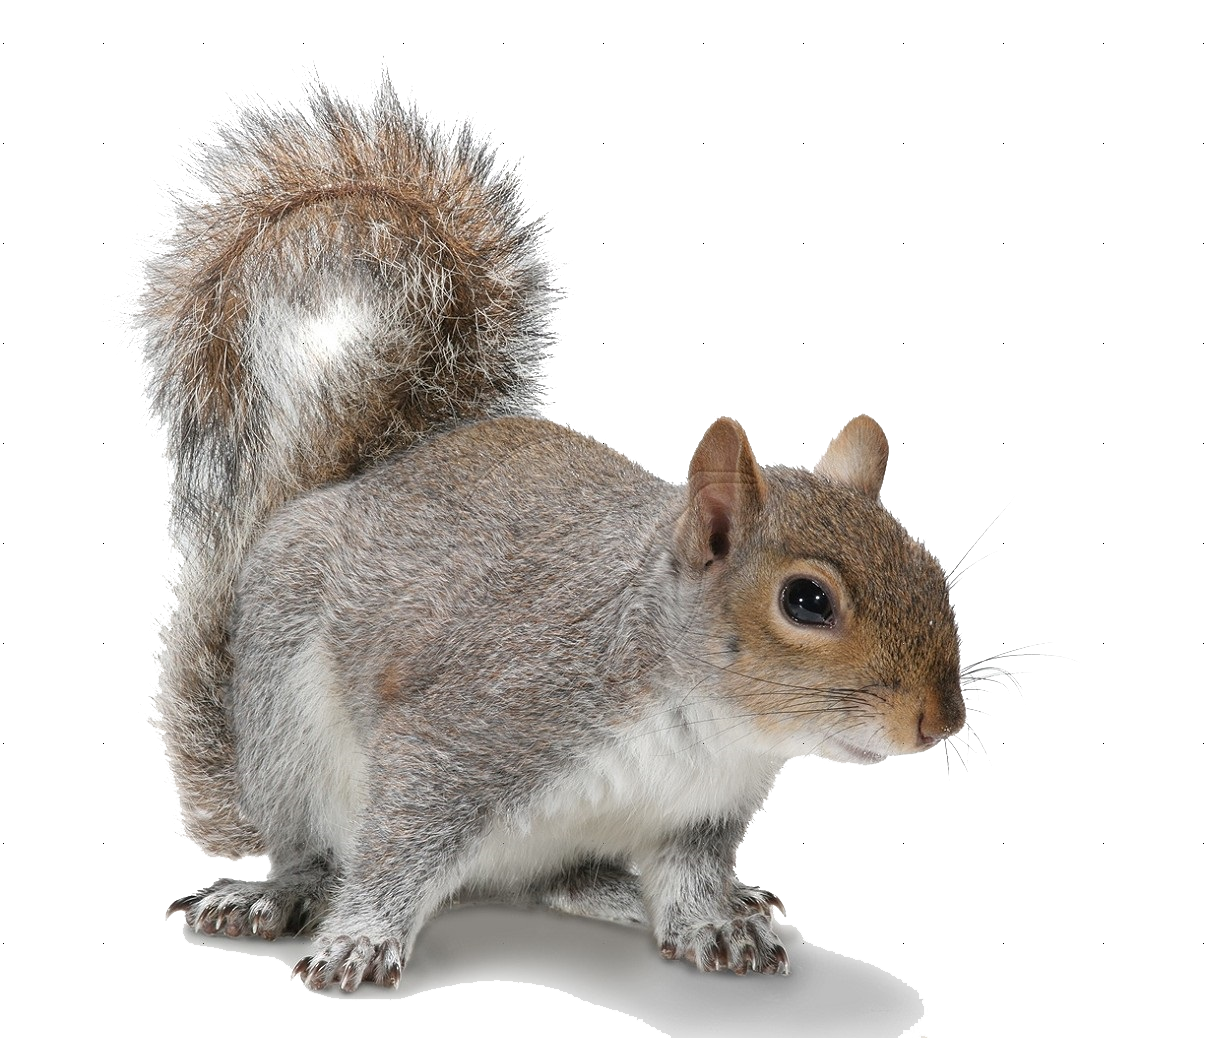
\includegraphics[height=3em]{../figures/squirrel.png} \\
\bottomrule
\end{tblr}
\end{table}

In HTML tables, it is possible to insert tables directly from a web
address, but not in LaTeX.

\subsection{Inline plots}\label{inline-plots}

We can draw inline plots three ways, with

\begin{enumerate}
\def\labelenumi{\arabic{enumi}.}
\tightlist
\item
  Built-in templates for histograms, density plots, and bar plots
\item
  Custom plots using base \texttt{R} plots.
\item
  Custom plots using \texttt{ggplot2}.
\end{enumerate}

To draw custom plots, one simply has to define a custom function, whose
structure we illustrate below.

\subsubsection{Built-in plots}\label{built-in-plots}

There are several types of inline plots available by default. For
example,

\begin{Shaded}
\begin{Highlighting}[]
\NormalTok{plot\_data }\OtherTok{\textless{}{-}} \FunctionTok{list}\NormalTok{(mtcars}\SpecialCharTok{$}\NormalTok{mpg, mtcars}\SpecialCharTok{$}\NormalTok{hp, mtcars}\SpecialCharTok{$}\NormalTok{qsec)}

\NormalTok{dat }\OtherTok{\textless{}{-}} \FunctionTok{data.frame}\NormalTok{(}
  \AttributeTok{Variables =} \FunctionTok{c}\NormalTok{(}\StringTok{"mpg"}\NormalTok{, }\StringTok{"hp"}\NormalTok{, }\StringTok{"qsec"}\NormalTok{), }
  \AttributeTok{Histogram =} \StringTok{""}\NormalTok{,}
  \AttributeTok{Density =} \StringTok{""}\NormalTok{,}
  \AttributeTok{Bar =} \StringTok{""}\NormalTok{,}
  \AttributeTok{Line =} \StringTok{""}
\NormalTok{)}

\CommentTok{\# random data for sparklines}
\NormalTok{lines }\OtherTok{\textless{}{-}} \FunctionTok{lapply}\NormalTok{(}\DecValTok{1}\SpecialCharTok{:}\DecValTok{3}\NormalTok{, \textbackslash{}(x) }\FunctionTok{data.frame}\NormalTok{(}\AttributeTok{x =} \DecValTok{1}\SpecialCharTok{:}\DecValTok{10}\NormalTok{, }\AttributeTok{y =} \FunctionTok{rnorm}\NormalTok{(}\DecValTok{10}\NormalTok{)))}

\FunctionTok{tt}\NormalTok{(dat) }\SpecialCharTok{|\textgreater{}}
  \FunctionTok{plot\_tt}\NormalTok{(}\AttributeTok{j =} \DecValTok{2}\NormalTok{, }\AttributeTok{fun =} \StringTok{"histogram"}\NormalTok{, }\AttributeTok{data =}\NormalTok{ plot\_data) }\SpecialCharTok{|\textgreater{}}
  \FunctionTok{plot\_tt}\NormalTok{(}\AttributeTok{j =} \DecValTok{3}\NormalTok{, }\AttributeTok{fun =} \StringTok{"density"}\NormalTok{, }\AttributeTok{data =}\NormalTok{ plot\_data, }\AttributeTok{color =} \StringTok{"darkgreen"}\NormalTok{) }\SpecialCharTok{|\textgreater{}}
  \FunctionTok{plot\_tt}\NormalTok{(}\AttributeTok{j =} \DecValTok{4}\NormalTok{, }\AttributeTok{fun =} \StringTok{"bar"}\NormalTok{, }\AttributeTok{data =} \FunctionTok{list}\NormalTok{(}\DecValTok{2}\NormalTok{, }\DecValTok{3}\NormalTok{, }\DecValTok{6}\NormalTok{), }\AttributeTok{color =} \StringTok{"orange"}\NormalTok{) }\SpecialCharTok{|\textgreater{}}
  \FunctionTok{plot\_tt}\NormalTok{(}\AttributeTok{j =} \DecValTok{5}\NormalTok{, }\AttributeTok{fun =} \StringTok{"line"}\NormalTok{, }\AttributeTok{data =}\NormalTok{ lines, }\AttributeTok{color =} \StringTok{"blue"}\NormalTok{) }\SpecialCharTok{|\textgreater{}}
  \FunctionTok{style\_tt}\NormalTok{(}\AttributeTok{j =} \DecValTok{2}\SpecialCharTok{:}\DecValTok{5}\NormalTok{, }\AttributeTok{align =} \StringTok{"c"}\NormalTok{)}
\end{Highlighting}
\end{Shaded}

\begin{table}[H]
\centering
\begin{tblr}[         %% tabularray outer open
]                     %% tabularray outer close
{                     %% tabularray inner open
colspec={Q[]Q[]Q[]Q[]Q[]},
column{2}={halign=c,},
column{3}={halign=c,},
column{4}={halign=c,},
column{5}={halign=c,},
}                     %% tabularray inner close
\toprule
Variables & Histogram & Density & Bar & Line \\ \midrule %% TinyTableHeader
mpg  & \includegraphics[height=1em]{tinytable_assets/idkq23crfxebxq76jae5eb.png} & \includegraphics[height=1em]{tinytable_assets/idhycmfhlg2g0kyaofw326.png} & \includegraphics[height=1em]{tinytable_assets/id8fy7lrsllp1tp17e8eqi.png} & \includegraphics[height=1em]{tinytable_assets/idd649181odtoirj418fi3.png} \\
hp   & \includegraphics[height=1em]{tinytable_assets/idr4bhy7czxt8wqxjkds3o.png} & \includegraphics[height=1em]{tinytable_assets/id5rv6dpovo0rijls9yyt4.png} & \includegraphics[height=1em]{tinytable_assets/idxrjdz8xk5894s33m3af5.png} & \includegraphics[height=1em]{tinytable_assets/idd9x9a59qihagjxn45amq.png} \\
qsec & \includegraphics[height=1em]{tinytable_assets/idssye5hf70qd93mubsh2s.png} & \includegraphics[height=1em]{tinytable_assets/id1ga0c31yl2l46b9jvd38.png} & \includegraphics[height=1em]{tinytable_assets/idids7hq6n33xzg00psv8n.png} & \includegraphics[height=1em]{tinytable_assets/idfsz5eq03e47f8lawdr1b.png} \\
\bottomrule
\end{tblr}
\end{table}

\subsubsection{\texorpdfstring{Custom plots: Base
\texttt{R}}{Custom plots: Base R}}\label{custom-plots-base-r}

Important: Custom functions must have \texttt{...} as an argument.

To create a custom inline plot using Base \texttt{R} plotting functions,
we create a function that returns another function. \texttt{tinytable}
will then call that second function internally to generate the plot.

This is easier than it sounds! For example:

\begin{Shaded}
\begin{Highlighting}[]
\NormalTok{f }\OtherTok{\textless{}{-}} \ControlFlowTok{function}\NormalTok{(d, ...) \{}
  \ControlFlowTok{function}\NormalTok{() }\FunctionTok{hist}\NormalTok{(d, }\AttributeTok{axes =} \ConstantTok{FALSE}\NormalTok{, }\AttributeTok{ann =} \ConstantTok{FALSE}\NormalTok{, }\AttributeTok{col =} \StringTok{"lightblue"}\NormalTok{)}
\NormalTok{\}}

\NormalTok{plot\_data }\OtherTok{\textless{}{-}} \FunctionTok{list}\NormalTok{(mtcars}\SpecialCharTok{$}\NormalTok{mpg, mtcars}\SpecialCharTok{$}\NormalTok{hp, mtcars}\SpecialCharTok{$}\NormalTok{qsec)}

\NormalTok{dat }\OtherTok{\textless{}{-}} \FunctionTok{data.frame}\NormalTok{(}\AttributeTok{Variables =} \FunctionTok{c}\NormalTok{(}\StringTok{"mpg"}\NormalTok{, }\StringTok{"hp"}\NormalTok{, }\StringTok{"qsec"}\NormalTok{), }\AttributeTok{Histogram =} \StringTok{""}\NormalTok{)}

\FunctionTok{tt}\NormalTok{(dat) }\SpecialCharTok{|\textgreater{}}
  \FunctionTok{plot\_tt}\NormalTok{(}\AttributeTok{j =} \DecValTok{2}\NormalTok{, }\AttributeTok{fun =}\NormalTok{ f, }\AttributeTok{data =}\NormalTok{ plot\_data)}
\end{Highlighting}
\end{Shaded}

\begin{table}[H]
\centering
\begin{tblr}[         %% tabularray outer open
]                     %% tabularray outer close
{                     %% tabularray inner open
colspec={Q[]Q[]},
}                     %% tabularray inner close
\toprule
Variables & Histogram \\ \midrule %% TinyTableHeader
mpg  & \includegraphics[height=1em]{tinytable_assets/idlqgta94z18lgqniz06dg.png} \\
hp   & \includegraphics[height=1em]{tinytable_assets/id1lxcu0rlx0vxbd3xxrmg.png} \\
qsec & \includegraphics[height=1em]{tinytable_assets/idm7zcfpkebavij41nbbez.png} \\
\bottomrule
\end{tblr}
\end{table}

\subsubsection{\texorpdfstring{Custom plots:
\texttt{ggplot2}}{Custom plots: ggplot2}}\label{custom-plots-ggplot2}

Important: Custom functions must have \texttt{...} as an argument.

To create a custom inline plot using \texttt{ggplot2}, we create a
function that returns a \texttt{ggplot} object:

\begin{Shaded}
\begin{Highlighting}[]
\FunctionTok{library}\NormalTok{(ggplot2)}

\NormalTok{f }\OtherTok{\textless{}{-}} \ControlFlowTok{function}\NormalTok{(d, }\AttributeTok{color =} \StringTok{"black"}\NormalTok{, ...) \{}
\NormalTok{  d }\OtherTok{\textless{}{-}} \FunctionTok{data.frame}\NormalTok{(}\AttributeTok{x =}\NormalTok{ d)}
  \FunctionTok{ggplot}\NormalTok{(d, }\FunctionTok{aes}\NormalTok{(}\AttributeTok{x =}\NormalTok{ x)) }\SpecialCharTok{+} 
    \FunctionTok{geom\_histogram}\NormalTok{(}\AttributeTok{bins =} \DecValTok{30}\NormalTok{, }\AttributeTok{color =}\NormalTok{ color, }\AttributeTok{fill =}\NormalTok{ color) }\SpecialCharTok{+}
    \FunctionTok{scale\_x\_continuous}\NormalTok{(}\AttributeTok{expand=}\FunctionTok{c}\NormalTok{(}\DecValTok{0}\NormalTok{,}\DecValTok{0}\NormalTok{)) }\SpecialCharTok{+}
    \FunctionTok{scale\_y\_continuous}\NormalTok{(}\AttributeTok{expand=}\FunctionTok{c}\NormalTok{(}\DecValTok{0}\NormalTok{,}\DecValTok{0}\NormalTok{)) }\SpecialCharTok{+}
    \FunctionTok{theme\_void}\NormalTok{()}
\NormalTok{\}}

\NormalTok{plot\_data }\OtherTok{\textless{}{-}} \FunctionTok{list}\NormalTok{(mtcars}\SpecialCharTok{$}\NormalTok{mpg, mtcars}\SpecialCharTok{$}\NormalTok{hp, mtcars}\SpecialCharTok{$}\NormalTok{qsec)}

\FunctionTok{tt}\NormalTok{(dat) }\SpecialCharTok{|\textgreater{}}
  \FunctionTok{plot\_tt}\NormalTok{(}\AttributeTok{j =} \DecValTok{2}\NormalTok{, }\AttributeTok{fun =}\NormalTok{ f, }\AttributeTok{data =}\NormalTok{ plot\_data, }\AttributeTok{color =} \StringTok{"pink"}\NormalTok{)}
\end{Highlighting}
\end{Shaded}

\begin{table}[H]
\centering
\begin{tblr}[         %% tabularray outer open
]                     %% tabularray outer close
{                     %% tabularray inner open
colspec={Q[]Q[]},
}                     %% tabularray inner close
\toprule
Variables & Histogram \\ \midrule %% TinyTableHeader
mpg  & \includegraphics[height=1em]{tinytable_assets/id723dt7jrd711si6up73t.png} \\
hp   & \includegraphics[height=1em]{tinytable_assets/id6aqbq2m14xqxhvjed6a8.png} \\
qsec & \includegraphics[height=1em]{tinytable_assets/idngncmful7iv8pcla4c05.png} \\
\bottomrule
\end{tblr}
\end{table}

We can insert arbitrarily complex plots by customizing the
\texttt{ggplot2} call:

\begin{Shaded}
\begin{Highlighting}[]
\NormalTok{penguins }\OtherTok{\textless{}{-}} \FunctionTok{read.csv}\NormalTok{(}
  \StringTok{"https://vincentarelbundock.github.io/Rdatasets/csv/palmerpenguins/penguins.csv"}\NormalTok{,}
  \AttributeTok{na.strings =} \StringTok{""}\NormalTok{) }\SpecialCharTok{|\textgreater{}} \FunctionTok{na.omit}\NormalTok{()}

\CommentTok{\# split data by species}
\NormalTok{dat }\OtherTok{\textless{}{-}} \FunctionTok{split}\NormalTok{(penguins, penguins}\SpecialCharTok{$}\NormalTok{species)}
\NormalTok{body }\OtherTok{\textless{}{-}} \FunctionTok{lapply}\NormalTok{(dat, \textbackslash{}(x) x}\SpecialCharTok{$}\NormalTok{body\_mass\_g)}
\NormalTok{flip }\OtherTok{\textless{}{-}} \FunctionTok{lapply}\NormalTok{(dat, \textbackslash{}(x) x}\SpecialCharTok{$}\NormalTok{flipper\_length\_mm)}

\CommentTok{\# create nearly empty table}
\NormalTok{tab }\OtherTok{\textless{}{-}} \FunctionTok{data.frame}\NormalTok{(}
  \StringTok{"Species"} \OtherTok{=} \FunctionTok{names}\NormalTok{(dat),}
  \StringTok{"Body Mass"} \OtherTok{=} \StringTok{""}\NormalTok{,}
  \StringTok{"Flipper Length"} \OtherTok{=} \StringTok{""}\NormalTok{,}
  \StringTok{"Body vs. Flipper"} \OtherTok{=} \StringTok{""}\NormalTok{,}
  \AttributeTok{check.names =} \ConstantTok{FALSE}
\NormalTok{)}

\CommentTok{\# custom ggplot2 function to create inline plot}
\NormalTok{f }\OtherTok{\textless{}{-}} \ControlFlowTok{function}\NormalTok{(d, ...) \{}
  \FunctionTok{ggplot}\NormalTok{(d, }\FunctionTok{aes}\NormalTok{(}\AttributeTok{x =}\NormalTok{ flipper\_length\_mm, }\AttributeTok{y =}\NormalTok{ body\_mass\_g, }\AttributeTok{color =}\NormalTok{ sex)) }\SpecialCharTok{+}
    \FunctionTok{geom\_point}\NormalTok{(}\AttributeTok{size =}\NormalTok{ .}\DecValTok{2}\NormalTok{) }\SpecialCharTok{+}
    \FunctionTok{scale\_x\_continuous}\NormalTok{(}\AttributeTok{expand=}\FunctionTok{c}\NormalTok{(}\DecValTok{0}\NormalTok{,}\DecValTok{0}\NormalTok{)) }\SpecialCharTok{+}
    \FunctionTok{scale\_y\_continuous}\NormalTok{(}\AttributeTok{expand=}\FunctionTok{c}\NormalTok{(}\DecValTok{0}\NormalTok{,}\DecValTok{0}\NormalTok{)) }\SpecialCharTok{+}
    \FunctionTok{scale\_color\_manual}\NormalTok{(}\AttributeTok{values =} \FunctionTok{c}\NormalTok{(}\StringTok{"\#E69F00"}\NormalTok{, }\StringTok{"\#56B4E9"}\NormalTok{)) }\SpecialCharTok{+}
    \FunctionTok{theme\_void}\NormalTok{() }\SpecialCharTok{+}
    \FunctionTok{theme}\NormalTok{(}\AttributeTok{legend.position =} \StringTok{"none"}\NormalTok{)}
\NormalTok{\}}

\CommentTok{\# \textasciigrave{}tinytable\textasciigrave{} calls}
\FunctionTok{tt}\NormalTok{(tab) }\SpecialCharTok{|\textgreater{}}
  \FunctionTok{plot\_tt}\NormalTok{(}\AttributeTok{j =} \DecValTok{2}\NormalTok{, }\AttributeTok{fun =} \StringTok{"histogram"}\NormalTok{, }\AttributeTok{data =}\NormalTok{ body, }\AttributeTok{height =} \DecValTok{2}\NormalTok{) }\SpecialCharTok{|\textgreater{}}
  \FunctionTok{plot\_tt}\NormalTok{(}\AttributeTok{j =} \DecValTok{3}\NormalTok{, }\AttributeTok{fun =} \StringTok{"density"}\NormalTok{, }\AttributeTok{data =}\NormalTok{ flip, }\AttributeTok{height =} \DecValTok{2}\NormalTok{) }\SpecialCharTok{|\textgreater{}}
  \FunctionTok{plot\_tt}\NormalTok{(}\AttributeTok{j =} \DecValTok{4}\NormalTok{, }\AttributeTok{fun =}\NormalTok{ f, }\AttributeTok{data =}\NormalTok{ dat, }\AttributeTok{height =} \DecValTok{2}\NormalTok{) }\SpecialCharTok{|\textgreater{}}
  \FunctionTok{style\_tt}\NormalTok{(}\AttributeTok{j =} \DecValTok{2}\SpecialCharTok{:}\DecValTok{4}\NormalTok{, }\AttributeTok{align =} \StringTok{"c"}\NormalTok{) }
\end{Highlighting}
\end{Shaded}

\begin{table}[H]
\centering
\begin{tblr}[         %% tabularray outer open
]                     %% tabularray outer close
{                     %% tabularray inner open
colspec={Q[]Q[]Q[]Q[]},
column{2}={halign=c,},
column{3}={halign=c,},
column{4}={halign=c,},
}                     %% tabularray inner close
\toprule
Species & Body Mass & Flipper Length & Body vs. Flipper \\ \midrule %% TinyTableHeader
Adelie    & \includegraphics[height=2em]{tinytable_assets/idegwb1daipi18d0rpdltc.png} & \includegraphics[height=2em]{tinytable_assets/iduoryjcer2pb5g1axgc47.png} & \includegraphics[height=2em]{tinytable_assets/idqrpne2wcna3wqvvji8ns.png} \\
Chinstrap & \includegraphics[height=2em]{tinytable_assets/idzxx4b9vphs8q00igwq98.png} & \includegraphics[height=2em]{tinytable_assets/idy9fiyhtbg6rt72xcfk3b.png} & \includegraphics[height=2em]{tinytable_assets/id575z88kp0v14uyii85kw.png} \\
Gentoo    & \includegraphics[height=2em]{tinytable_assets/idc7hs4qyog4dkqlhra8xa.png} & \includegraphics[height=2em]{tinytable_assets/idypeexj0c1h235ipwdrxr.png} & \includegraphics[height=2em]{tinytable_assets/id9fr1j9m78n18dpr6itll.png} \\
\bottomrule
\end{tblr}
\end{table}

\section{Groups and labels}\label{groups-and-labels}

The \texttt{group\_tt()} function can label groups of rows (\texttt{i})
or columns (\texttt{j}).

\subsection{Rows}\label{rows}

The \texttt{i} argument accepts a named list of integers. The numbers
identify the positions where row group labels are to be inserted. The
names includes the text that should be inserted:

\begin{Shaded}
\begin{Highlighting}[]
\NormalTok{dat }\OtherTok{\textless{}{-}}\NormalTok{ mtcars[}\DecValTok{1}\SpecialCharTok{:}\DecValTok{9}\NormalTok{, }\DecValTok{1}\SpecialCharTok{:}\DecValTok{8}\NormalTok{]}

\FunctionTok{tt}\NormalTok{(dat) }\SpecialCharTok{|\textgreater{}}
  \FunctionTok{group\_tt}\NormalTok{(}\AttributeTok{i =} \FunctionTok{list}\NormalTok{(}
    \StringTok{"I like (fake) hamburgers"} \OtherTok{=} \DecValTok{3}\NormalTok{,}
    \StringTok{"She prefers halloumi"} \OtherTok{=} \DecValTok{4}\NormalTok{,}
    \StringTok{"They love tofu"} \OtherTok{=} \DecValTok{7}\NormalTok{))}
\end{Highlighting}
\end{Shaded}

\begin{table}[H]
\centering
\begin{tblr}[         %% tabularray outer open
]                     %% tabularray outer close
{                     %% tabularray inner open
colspec={Q[]Q[]Q[]Q[]Q[]Q[]Q[]Q[]},
cell{4}{1}={c=8}{},cell{6}{1}={c=8}{},cell{10}{1}={c=8}{},
cell{2}{1}={preto={\hspace{1em}}},
cell{3}{1}={preto={\hspace{1em}}},
cell{5}{1}={preto={\hspace{1em}}},
cell{7}{1}={preto={\hspace{1em}}},
cell{8}{1}={preto={\hspace{1em}}},
cell{9}{1}={preto={\hspace{1em}}},
cell{11}{1}={preto={\hspace{1em}}},
cell{12}{1}={preto={\hspace{1em}}},
cell{13}{1}={preto={\hspace{1em}}},
cell{14}{1}={preto={\hspace{1em}}},
}                     %% tabularray inner close
\toprule
mpg & cyl & disp & hp & drat & wt & qsec & vs \\ \midrule %% TinyTableHeader
21.0 & 6 & 160.0 & 110 & 3.90 & 2.620 & 16.46 & 0 \\
21.0 & 6 & 160.0 & 110 & 3.90 & 2.875 & 17.02 & 0 \\
I like (fake) hamburgers &&&&&&&& \\
22.8 & 4 & 108.0 &  93 & 3.85 & 2.320 & 18.61 & 1 \\
She prefers halloumi &&&&&&&& \\
21.4 & 6 & 258.0 & 110 & 3.08 & 3.215 & 19.44 & 1 \\
18.7 & 8 & 360.0 & 175 & 3.15 & 3.440 & 17.02 & 0 \\
18.1 & 6 & 225.0 & 105 & 2.76 & 3.460 & 20.22 & 1 \\
They love tofu &&&&&&&& \\
14.3 & 8 & 360.0 & 245 & 3.21 & 3.570 & 15.84 & 0 \\
24.4 & 4 & 146.7 &  62 & 3.69 & 3.190 & 20.00 & 1 \\
22.8 & 4 & 140.8 &  95 & 3.92 & 3.150 & 22.90 & 1 \\
\bottomrule
\end{tblr}
\end{table}

We can style group rows in the same way as regular rows:

\begin{Shaded}
\begin{Highlighting}[]
\FunctionTok{tt}\NormalTok{(dat) }\SpecialCharTok{|\textgreater{}} 
  \FunctionTok{group\_tt}\NormalTok{(}
    \AttributeTok{i =} \FunctionTok{list}\NormalTok{(}
      \StringTok{"I like (fake) hamburgers"} \OtherTok{=} \DecValTok{3}\NormalTok{,}
      \StringTok{"She prefers halloumi"} \OtherTok{=} \DecValTok{4}\NormalTok{,}
      \StringTok{"They love tofu"} \OtherTok{=} \DecValTok{7}\NormalTok{)) }\SpecialCharTok{|\textgreater{}}
  \FunctionTok{style\_tt}\NormalTok{(}
    \AttributeTok{i =} \FunctionTok{c}\NormalTok{(}\DecValTok{3}\NormalTok{, }\DecValTok{5}\NormalTok{, }\DecValTok{9}\NormalTok{),}
    \AttributeTok{align =} \StringTok{"c"}\NormalTok{,}
    \AttributeTok{color =} \StringTok{"white"}\NormalTok{,}
    \AttributeTok{background =} \StringTok{"gray"}\NormalTok{,}
    \AttributeTok{bold =} \ConstantTok{TRUE}\NormalTok{)}
\end{Highlighting}
\end{Shaded}

\begin{table}[H]
\centering
\begin{tblr}[         %% tabularray outer open
]                     %% tabularray outer close
{                     %% tabularray inner open
colspec={Q[]Q[]Q[]Q[]Q[]Q[]Q[]Q[]},
cell{4}{1}={c=8}{},cell{6}{1}={c=8}{},cell{10}{1}={c=8}{},
cell{2}{1}={preto={\hspace{1em}}},
cell{3}{1}={preto={\hspace{1em}}},
cell{5}{1}={preto={\hspace{1em}}},
cell{7}{1}={preto={\hspace{1em}}},
cell{8}{1}={preto={\hspace{1em}}},
cell{9}{1}={preto={\hspace{1em}}},
cell{11}{1}={preto={\hspace{1em}}},
cell{12}{1}={preto={\hspace{1em}}},
cell{13}{1}={preto={\hspace{1em}}},
cell{14}{1}={preto={\hspace{1em}}},
row{4}={halign=c,cmd=\bfseries,bg=gray,fg=white,},
row{6}={halign=c,cmd=\bfseries,bg=gray,fg=white,},
row{10}={halign=c,cmd=\bfseries,bg=gray,fg=white,},
}                     %% tabularray inner close
\toprule
mpg & cyl & disp & hp & drat & wt & qsec & vs \\ \midrule %% TinyTableHeader
21.0 & 6 & 160.0 & 110 & 3.90 & 2.620 & 16.46 & 0 \\
21.0 & 6 & 160.0 & 110 & 3.90 & 2.875 & 17.02 & 0 \\
I like (fake) hamburgers &&&&&&&& \\
22.8 & 4 & 108.0 &  93 & 3.85 & 2.320 & 18.61 & 1 \\
She prefers halloumi &&&&&&&& \\
21.4 & 6 & 258.0 & 110 & 3.08 & 3.215 & 19.44 & 1 \\
18.7 & 8 & 360.0 & 175 & 3.15 & 3.440 & 17.02 & 0 \\
18.1 & 6 & 225.0 & 105 & 2.76 & 3.460 & 20.22 & 1 \\
They love tofu &&&&&&&& \\
14.3 & 8 & 360.0 & 245 & 3.21 & 3.570 & 15.84 & 0 \\
24.4 & 4 & 146.7 &  62 & 3.69 & 3.190 & 20.00 & 1 \\
22.8 & 4 & 140.8 &  95 & 3.92 & 3.150 & 22.90 & 1 \\
\bottomrule
\end{tblr}
\end{table}

\subsection{Columns}\label{columns}

The syntax for column groups is very similar, but we use the \texttt{j}
argument instead. The named list specifies the labels to appear in
column-spanning labels, and the values must be a vector of consecutive
and non-overlapping integers that indicate which columns are associated
to which labels:

\begin{Shaded}
\begin{Highlighting}[]
\FunctionTok{tt}\NormalTok{(dat) }\SpecialCharTok{|\textgreater{}} 
  \FunctionTok{group\_tt}\NormalTok{(}
    \AttributeTok{j =} \FunctionTok{list}\NormalTok{(}
      \StringTok{"Hamburgers"} \OtherTok{=} \DecValTok{1}\SpecialCharTok{:}\DecValTok{3}\NormalTok{,}
      \StringTok{"Halloumi"} \OtherTok{=} \DecValTok{4}\SpecialCharTok{:}\DecValTok{5}\NormalTok{,}
      \StringTok{"Tofu"} \OtherTok{=} \DecValTok{7}\NormalTok{))}
\end{Highlighting}
\end{Shaded}

\begin{table}[H]
\centering
\begin{tblr}[         %% tabularray outer open
]                     %% tabularray outer close
{                     %% tabularray inner open
colspec={Q[]Q[]Q[]Q[]Q[]Q[]Q[]Q[]},
cell{1}{1}={c=3,}{halign=c,},
cell{1}{4}={c=2,}{halign=c,},
cell{1}{7}={c=1,}{halign=c,},
}                     %% tabularray inner close
\toprule
Hamburgers &  &  & Halloumi &  &  & Tofu &  \\ \cmidrule[lr]{1-3}\cmidrule[lr]{4-5}\cmidrule[lr]{7-7}
mpg & cyl & disp & hp & drat & wt & qsec & vs \\ \midrule %% TinyTableHeader
21.0 & 6 & 160.0 & 110 & 3.90 & 2.620 & 16.46 & 0 \\
21.0 & 6 & 160.0 & 110 & 3.90 & 2.875 & 17.02 & 0 \\
22.8 & 4 & 108.0 &  93 & 3.85 & 2.320 & 18.61 & 1 \\
21.4 & 6 & 258.0 & 110 & 3.08 & 3.215 & 19.44 & 1 \\
18.7 & 8 & 360.0 & 175 & 3.15 & 3.440 & 17.02 & 0 \\
18.1 & 6 & 225.0 & 105 & 2.76 & 3.460 & 20.22 & 1 \\
14.3 & 8 & 360.0 & 245 & 3.21 & 3.570 & 15.84 & 0 \\
24.4 & 4 & 146.7 &  62 & 3.69 & 3.190 & 20.00 & 1 \\
22.8 & 4 & 140.8 &  95 & 3.92 & 3.150 & 22.90 & 1 \\
\bottomrule
\end{tblr}
\end{table}

Here is a table with both row and column headers, as well as some
styling:

\begin{Shaded}
\begin{Highlighting}[]
\NormalTok{dat }\OtherTok{\textless{}{-}}\NormalTok{ mtcars[}\DecValTok{1}\SpecialCharTok{:}\DecValTok{9}\NormalTok{, }\DecValTok{1}\SpecialCharTok{:}\DecValTok{8}\NormalTok{]}
\FunctionTok{tt}\NormalTok{(dat) }\SpecialCharTok{|\textgreater{}} 
  \FunctionTok{group\_tt}\NormalTok{(}
    \AttributeTok{i =} \FunctionTok{list}\NormalTok{(}\StringTok{"I like (fake) hamburgers"} \OtherTok{=} \DecValTok{3}\NormalTok{,}
             \StringTok{"She prefers halloumi"} \OtherTok{=} \DecValTok{4}\NormalTok{,}
             \StringTok{"They love tofu"} \OtherTok{=} \DecValTok{7}\NormalTok{),}
    \AttributeTok{j =} \FunctionTok{list}\NormalTok{(}\StringTok{"Hamburgers"} \OtherTok{=} \DecValTok{1}\SpecialCharTok{:}\DecValTok{3}\NormalTok{,}
             \StringTok{"Halloumi"} \OtherTok{=} \DecValTok{4}\SpecialCharTok{:}\DecValTok{5}\NormalTok{,}
             \StringTok{"Tofu"} \OtherTok{=} \DecValTok{7}\NormalTok{)) }\SpecialCharTok{|\textgreater{}}
  \FunctionTok{style\_tt}\NormalTok{(}
    \AttributeTok{i =} \FunctionTok{c}\NormalTok{(}\DecValTok{3}\NormalTok{, }\DecValTok{5}\NormalTok{, }\DecValTok{9}\NormalTok{),}
    \AttributeTok{align =} \StringTok{"c"}\NormalTok{,}
    \AttributeTok{background =} \StringTok{"teal"}\NormalTok{,}
    \AttributeTok{color =} \StringTok{"white"}\NormalTok{) }\SpecialCharTok{|\textgreater{}}
  \FunctionTok{style\_tt}\NormalTok{(}\AttributeTok{i =} \SpecialCharTok{{-}}\DecValTok{1}\NormalTok{, }\AttributeTok{color =} \StringTok{"teal"}\NormalTok{)}
\end{Highlighting}
\end{Shaded}

\begin{table}[H]
\centering
\begin{tblr}[         %% tabularray outer open
]                     %% tabularray outer close
{                     %% tabularray inner open
colspec={Q[]Q[]Q[]Q[]Q[]Q[]Q[]Q[]},
cell{1}{1}={c=3,}{halign=c,},
cell{1}{4}={c=2,}{halign=c,},
cell{1}{7}={c=1,}{halign=c,},
cell{5}{1}={c=8}{},cell{7}{1}={c=8}{},cell{11}{1}={c=8}{},
cell{3}{1}={preto={\hspace{1em}}},
cell{4}{1}={preto={\hspace{1em}}},
cell{6}{1}={preto={\hspace{1em}}},
cell{8}{1}={preto={\hspace{1em}}},
cell{9}{1}={preto={\hspace{1em}}},
cell{10}{1}={preto={\hspace{1em}}},
cell{12}{1}={preto={\hspace{1em}}},
cell{13}{1}={preto={\hspace{1em}}},
cell{14}{1}={preto={\hspace{1em}}},
cell{15}{1}={preto={\hspace{1em}}},
row{5}={halign=c,bg=teal,fg=white,},
row{7}={halign=c,bg=teal,fg=white,},
row{11}={halign=c,bg=teal,fg=white,},
row{1}={,fg=teal,},
}                     %% tabularray inner close
\toprule
Hamburgers &  &  & Halloumi &  &  & Tofu &  \\ \cmidrule[lr]{1-3}\cmidrule[lr]{4-5}\cmidrule[lr]{7-7}
mpg & cyl & disp & hp & drat & wt & qsec & vs \\ \midrule %% TinyTableHeader
21.0 & 6 & 160.0 & 110 & 3.90 & 2.620 & 16.46 & 0 \\
21.0 & 6 & 160.0 & 110 & 3.90 & 2.875 & 17.02 & 0 \\
I like (fake) hamburgers &&&&&&&& \\
22.8 & 4 & 108.0 &  93 & 3.85 & 2.320 & 18.61 & 1 \\
She prefers halloumi &&&&&&&& \\
21.4 & 6 & 258.0 & 110 & 3.08 & 3.215 & 19.44 & 1 \\
18.7 & 8 & 360.0 & 175 & 3.15 & 3.440 & 17.02 & 0 \\
18.1 & 6 & 225.0 & 105 & 2.76 & 3.460 & 20.22 & 1 \\
They love tofu &&&&&&&& \\
14.3 & 8 & 360.0 & 245 & 3.21 & 3.570 & 15.84 & 0 \\
24.4 & 4 & 146.7 &  62 & 3.69 & 3.190 & 20.00 & 1 \\
22.8 & 4 & 140.8 &  95 & 3.92 & 3.150 & 22.90 & 1 \\
\bottomrule
\end{tblr}
\end{table}

We can also stack several extra headers on top of one another:

\begin{Shaded}
\begin{Highlighting}[]
\FunctionTok{tt}\NormalTok{(x) }\SpecialCharTok{|\textgreater{}}
  \FunctionTok{group\_tt}\NormalTok{(}\AttributeTok{j =} \FunctionTok{list}\NormalTok{(}\StringTok{"Foo"} \OtherTok{=} \DecValTok{2}\SpecialCharTok{:}\DecValTok{3}\NormalTok{, }\StringTok{"Bar"} \OtherTok{=} \DecValTok{5}\NormalTok{)) }\SpecialCharTok{|\textgreater{}}
  \FunctionTok{group\_tt}\NormalTok{(}\AttributeTok{j =} \FunctionTok{list}\NormalTok{(}\StringTok{"Hello"} \OtherTok{=} \DecValTok{1}\SpecialCharTok{:}\DecValTok{2}\NormalTok{, }\StringTok{"World"} \OtherTok{=} \DecValTok{4}\SpecialCharTok{:}\DecValTok{5}\NormalTok{))}
\end{Highlighting}
\end{Shaded}

\begin{table}[H]
\centering
\begin{tblr}[         %% tabularray outer open
]                     %% tabularray outer close
{                     %% tabularray inner open
colspec={Q[]Q[]Q[]Q[]Q[]},
cell{2}{2}={c=2,}{halign=c,},
cell{2}{5}={c=1,}{halign=c,},
cell{1}{1}={c=2,}{halign=c,},
cell{1}{4}={c=2,}{halign=c,},
}                     %% tabularray inner close
\toprule
Hello &  &  & World &  \\ \cmidrule[lr]{1-2}\cmidrule[lr]{4-5}
& Foo &  &  & Bar \\ \cmidrule[lr]{2-3}\cmidrule[lr]{5-5}
mpg & cyl & disp & hp & drat \\ \midrule %% TinyTableHeader
21.0 & 6 & 160 & 110 & 3.90 \\
21.0 & 6 & 160 & 110 & 3.90 \\
22.8 & 4 & 108 &  93 & 3.85 \\
21.4 & 6 & 258 & 110 & 3.08 \\
\bottomrule
\end{tblr}
\end{table}

\section{Themes}\label{themes}

\texttt{tinytable} offers a very flexible theming framwork, which
includes a few basic visual looks, as well as other functions to apply
collections of transformations to \texttt{tinytable} objects in a
repeatable way. These themes can be applied by supplying a string or
function to the \texttt{theme} argument in \texttt{tt()}. Alternatively,
users can call the \texttt{theme\_tt()} function.

The main difference between \texttt{theme\_tt()} and the other options
in package, is that whereas \texttt{style\_tt()} and
\texttt{format\_tt()} aim to be output agnostic, \texttt{theme\_tt()}
supplies transformations that can be output-specific, and which can have
their own sets of distinct arguments. See below for a few examples.

\subsection{Visual themes}\label{visual-themes}

To begin, let's explore a few of the basic looks supplied by themes:

\begin{Shaded}
\begin{Highlighting}[]
\FunctionTok{tt}\NormalTok{(x, }\AttributeTok{theme =} \StringTok{"striped"}\NormalTok{)}
\end{Highlighting}
\end{Shaded}

\begin{table}[H]
\centering
\begin{tblr}[         %% tabularray outer open
]                     %% tabularray outer close
{                     %% tabularray inner open
colspec={Q[]Q[]Q[]Q[]Q[]},
row{even}={bg=black!5!white},
}                     %% tabularray inner close
\toprule
mpg & cyl & disp & hp & drat \\ \midrule %% TinyTableHeader
21.0 & 6 & 160 & 110 & 3.90 \\
21.0 & 6 & 160 & 110 & 3.90 \\
22.8 & 4 & 108 &  93 & 3.85 \\
21.4 & 6 & 258 & 110 & 3.08 \\
\bottomrule
\end{tblr}
\end{table}

\begin{Shaded}
\begin{Highlighting}[]
\FunctionTok{tt}\NormalTok{(x) }\SpecialCharTok{|\textgreater{}} \FunctionTok{theme\_tt}\NormalTok{(}\StringTok{"striped"}\NormalTok{)}
\end{Highlighting}
\end{Shaded}

\begin{table}[H]
\centering
\begin{tblr}[         %% tabularray outer open
]                     %% tabularray outer close
{                     %% tabularray inner open
colspec={Q[]Q[]Q[]Q[]Q[]},
row{even}={bg=black!5!white},
}                     %% tabularray inner close
\toprule
mpg & cyl & disp & hp & drat \\ \midrule %% TinyTableHeader
21.0 & 6 & 160 & 110 & 3.90 \\
21.0 & 6 & 160 & 110 & 3.90 \\
22.8 & 4 & 108 &  93 & 3.85 \\
21.4 & 6 & 258 & 110 & 3.08 \\
\bottomrule
\end{tblr}
\end{table}

\begin{Shaded}
\begin{Highlighting}[]
\FunctionTok{tt}\NormalTok{(x, }\AttributeTok{theme =} \StringTok{"grid"}\NormalTok{)}
\end{Highlighting}
\end{Shaded}

\begin{table}[H]
\centering
\begin{tblr}[         %% tabularray outer open
]                     %% tabularray outer close
{                     %% tabularray inner open
colspec={Q[]Q[]Q[]Q[]Q[]},
hlines, vlines,
}                     %% tabularray inner close
mpg & cyl & disp & hp & drat \\
21.0 & 6 & 160 & 110 & 3.90 \\
21.0 & 6 & 160 & 110 & 3.90 \\
22.8 & 4 & 108 &  93 & 3.85 \\
21.4 & 6 & 258 & 110 & 3.08 \\
\end{tblr}
\end{table}

\begin{Shaded}
\begin{Highlighting}[]
\FunctionTok{tt}\NormalTok{(x, }\AttributeTok{theme =} \StringTok{"bootstrap"}\NormalTok{)}
\end{Highlighting}
\end{Shaded}

\begin{table}[H]
\centering
\begin{tblr}[         %% tabularray outer open
]                     %% tabularray outer close
{                     %% tabularray inner open
colspec={Q[]Q[]Q[]Q[]Q[]},
hlines={gray8},
}                     %% tabularray inner close
mpg & cyl & disp & hp & drat \\
21.0 & 6 & 160 & 110 & 3.90 \\
21.0 & 6 & 160 & 110 & 3.90 \\
22.8 & 4 & 108 &  93 & 3.85 \\
21.4 & 6 & 258 & 110 & 3.08 \\
\end{tblr}
\end{table}

\begin{Shaded}
\begin{Highlighting}[]
\FunctionTok{tt}\NormalTok{(x, }\AttributeTok{theme =} \StringTok{"void"}\NormalTok{)}
\end{Highlighting}
\end{Shaded}

\begin{table}[H]
\centering
\begin{tblr}[         %% tabularray outer open
]                     %% tabularray outer close
{                     %% tabularray inner open
colspec={Q[]Q[]Q[]Q[]Q[]},
}                     %% tabularray inner close
mpg & cyl & disp & hp & drat \\
21.0 & 6 & 160 & 110 & 3.90 \\
21.0 & 6 & 160 & 110 & 3.90 \\
22.8 & 4 & 108 &  93 & 3.85 \\
21.4 & 6 & 258 & 110 & 3.08 \\
\end{tblr}
\end{table}

\subsection{Custom themes}\label{custom-themes}

Users can also define their own themes to apply consistent visual tweaks
to tables. For example, this defines a themeing function and sets a
global option to apply it to all tables consistently:

\begin{Shaded}
\begin{Highlighting}[]
\NormalTok{theme\_vincent }\OtherTok{\textless{}{-}} \ControlFlowTok{function}\NormalTok{(x, ...) \{}
\NormalTok{  out }\OtherTok{\textless{}{-}}\NormalTok{ x }\SpecialCharTok{|\textgreater{}} 
    \FunctionTok{style\_tt}\NormalTok{(}\AttributeTok{color =} \StringTok{"teal"}\NormalTok{) }\SpecialCharTok{|\textgreater{}}
    \FunctionTok{theme\_tt}\NormalTok{(}\StringTok{"placement"}\NormalTok{)}
\NormalTok{  out}\SpecialCharTok{@}\NormalTok{caption }\OtherTok{\textless{}{-}} \StringTok{"Always use the same caption."}
  \FunctionTok{return}\NormalTok{(out)}
\NormalTok{\}}

\FunctionTok{options}\NormalTok{(}\AttributeTok{tinytable\_tt\_theme =}\NormalTok{ theme\_vincent)}

\FunctionTok{tt}\NormalTok{(mtcars[}\DecValTok{1}\SpecialCharTok{:}\DecValTok{2}\NormalTok{, }\DecValTok{1}\SpecialCharTok{:}\DecValTok{2}\NormalTok{])}
\end{Highlighting}
\end{Shaded}

\begin{table}[H]
\caption{Always use the same caption.}
\centering
\begin{tblr}[         %% tabularray outer open
]                     %% tabularray outer close
{                     %% tabularray inner open
colspec={Q[]Q[]},
row{2}={,fg=teal,},
row{3}={,fg=teal,},
}                     %% tabularray inner close
\toprule
mpg & cyl \\ \midrule %% TinyTableHeader
21 & 6 \\
21 & 6 \\
\bottomrule
\end{tblr}
\end{table}

\begin{Shaded}
\begin{Highlighting}[]
\FunctionTok{tt}\NormalTok{(mtcars[}\DecValTok{1}\SpecialCharTok{:}\DecValTok{3}\NormalTok{, }\DecValTok{1}\SpecialCharTok{:}\DecValTok{3}\NormalTok{])}
\end{Highlighting}
\end{Shaded}

\begin{table}[H]
\caption{Always use the same caption.}
\centering
\begin{tblr}[         %% tabularray outer open
]                     %% tabularray outer close
{                     %% tabularray inner open
colspec={Q[]Q[]Q[]},
row{2}={,fg=teal,},
row{3}={,fg=teal,},
row{4}={,fg=teal,},
}                     %% tabularray inner close
\toprule
mpg & cyl & disp \\ \midrule %% TinyTableHeader
21.0 & 6 & 160 \\
21.0 & 6 & 160 \\
22.8 & 4 & 108 \\
\bottomrule
\end{tblr}
\end{table}

\begin{Shaded}
\begin{Highlighting}[]
\FunctionTok{options}\NormalTok{(}\AttributeTok{tinytable\_tt\_theme =} \ConstantTok{NULL}\NormalTok{)}
\end{Highlighting}
\end{Shaded}

\subsection{Tabular}\label{tabular}

The \texttt{tabular} theme is designed to provide a more ``raw'' table,
without a floating table environment in LaTeX, and without CSS or
Javascript in HTML.

\begin{Shaded}
\begin{Highlighting}[]
\FunctionTok{tt}\NormalTok{(x) }\SpecialCharTok{|\textgreater{}} \FunctionTok{theme\_tt}\NormalTok{(}\StringTok{"tabular"}\NormalTok{) }\SpecialCharTok{|\textgreater{}} \FunctionTok{print}\NormalTok{(}\StringTok{"latex"}\NormalTok{)}
\end{Highlighting}
\end{Shaded}

\begin{verbatim}
\begin{tblr}[         %% tabularray outer open
]                     %% tabularray outer close
{                     %% tabularray inner open
colspec={Q[]Q[]Q[]Q[]Q[]},
}                     %% tabularray inner close
\toprule
mpg & cyl & disp & hp & drat \\ \midrule %% TinyTableHeader
21.0 & 6 & 160 & 110 & 3.90 \\
21.0 & 6 & 160 & 110 & 3.90 \\
22.8 & 4 & 108 &  93 & 3.85 \\
21.4 & 6 & 258 & 110 & 3.08 \\
\bottomrule
\end{tblr} 
\end{verbatim}

\subsection{Resize}\label{resize}

The \texttt{resize} theme allows you to adjust the size of the table in
LaTeX outputs, making it fit within a specified width of the page. This
is useful for large tables that need to be scaled down to fit the
document layout. This table will be scaled to 90\% of the available line
width, ensuring it fits nicely within the document.

\begin{Shaded}
\begin{Highlighting}[]
\NormalTok{tmp }\OtherTok{\textless{}{-}} \FunctionTok{cbind}\NormalTok{(mtcars, mtcars)[}\DecValTok{1}\SpecialCharTok{:}\DecValTok{10}\NormalTok{,]}

\FunctionTok{tt}\NormalTok{(tmp) }\SpecialCharTok{|\textgreater{}} \FunctionTok{theme\_tt}\NormalTok{(}\StringTok{"resize"}\NormalTok{, }\AttributeTok{width =}\NormalTok{ .}\DecValTok{9}\NormalTok{)}
\end{Highlighting}
\end{Shaded}

\begin{table}[H]
\centering
\resizebox{\ifdim\width>\linewidth 0.9\linewidth\else\width\fi}{!}{
\begin{tblr}[         %% tabularray outer open
]                     %% tabularray outer close
{                     %% tabularray inner open
colspec={Q[]Q[]Q[]Q[]Q[]Q[]Q[]Q[]Q[]Q[]Q[]Q[]Q[]Q[]Q[]Q[]Q[]Q[]Q[]Q[]Q[]Q[]},
}                     %% tabularray inner close
\toprule
mpg & cyl & disp & hp & drat & wt & qsec & vs & am & gear & carb & mpg & cyl & disp & hp & drat & wt & qsec & vs & am & gear & carb \\ \midrule %% TinyTableHeader
21.0 & 6 & 160.0 & 110 & 3.90 & 2.620 & 16.46 & 0 & 1 & 4 & 4 & 21.0 & 6 & 160.0 & 110 & 3.90 & 2.620 & 16.46 & 0 & 1 & 4 & 4 \\
21.0 & 6 & 160.0 & 110 & 3.90 & 2.875 & 17.02 & 0 & 1 & 4 & 4 & 21.0 & 6 & 160.0 & 110 & 3.90 & 2.875 & 17.02 & 0 & 1 & 4 & 4 \\
22.8 & 4 & 108.0 &  93 & 3.85 & 2.320 & 18.61 & 1 & 1 & 4 & 1 & 22.8 & 4 & 108.0 &  93 & 3.85 & 2.320 & 18.61 & 1 & 1 & 4 & 1 \\
21.4 & 6 & 258.0 & 110 & 3.08 & 3.215 & 19.44 & 1 & 0 & 3 & 1 & 21.4 & 6 & 258.0 & 110 & 3.08 & 3.215 & 19.44 & 1 & 0 & 3 & 1 \\
18.7 & 8 & 360.0 & 175 & 3.15 & 3.440 & 17.02 & 0 & 0 & 3 & 2 & 18.7 & 8 & 360.0 & 175 & 3.15 & 3.440 & 17.02 & 0 & 0 & 3 & 2 \\
18.1 & 6 & 225.0 & 105 & 2.76 & 3.460 & 20.22 & 1 & 0 & 3 & 1 & 18.1 & 6 & 225.0 & 105 & 2.76 & 3.460 & 20.22 & 1 & 0 & 3 & 1 \\
14.3 & 8 & 360.0 & 245 & 3.21 & 3.570 & 15.84 & 0 & 0 & 3 & 4 & 14.3 & 8 & 360.0 & 245 & 3.21 & 3.570 & 15.84 & 0 & 0 & 3 & 4 \\
24.4 & 4 & 146.7 &  62 & 3.69 & 3.190 & 20.00 & 1 & 0 & 4 & 2 & 24.4 & 4 & 146.7 &  62 & 3.69 & 3.190 & 20.00 & 1 & 0 & 4 & 2 \\
22.8 & 4 & 140.8 &  95 & 3.92 & 3.150 & 22.90 & 1 & 0 & 4 & 2 & 22.8 & 4 & 140.8 &  95 & 3.92 & 3.150 & 22.90 & 1 & 0 & 4 & 2 \\
19.2 & 6 & 167.6 & 123 & 3.92 & 3.440 & 18.30 & 1 & 0 & 4 & 4 & 19.2 & 6 & 167.6 & 123 & 3.92 & 3.440 & 18.30 & 1 & 0 & 4 & 4 \\
\bottomrule
\end{tblr}
}
\end{table}

\subsection{Placement}\label{placement}

The \texttt{placement} theme offers control over the positioning of the
table in LaTeX documents, using floating parameters like \texttt{H}
(from the \texttt{float} LaTeX package) to specify where the table
should appear.

\begin{Shaded}
\begin{Highlighting}[]
\FunctionTok{tt}\NormalTok{(x) }\SpecialCharTok{|\textgreater{}}
  \FunctionTok{theme\_tt}\NormalTok{(}\StringTok{"placement"}\NormalTok{, }\AttributeTok{latex\_float =} \StringTok{"H"}\NormalTok{) }\SpecialCharTok{|\textgreater{}}
  \FunctionTok{print}\NormalTok{(}\AttributeTok{output =} \StringTok{"latex"}\NormalTok{)}
\end{Highlighting}
\end{Shaded}

\begin{verbatim}
\begin{table}[H]
\centering
\begin{tblr}[         %% tabularray outer open
]                     %% tabularray outer close
{                     %% tabularray inner open
colspec={Q[]Q[]Q[]Q[]Q[]},
}                     %% tabularray inner close
\toprule
mpg & cyl & disp & hp & drat \\ \midrule %% TinyTableHeader
21.0 & 6 & 160 & 110 & 3.90 \\
21.0 & 6 & 160 & 110 & 3.90 \\
22.8 & 4 & 108 &  93 & 3.85 \\
21.4 & 6 & 258 & 110 & 3.08 \\
\bottomrule
\end{tblr}
\end{table} 
\end{verbatim}

\subsection{Multipage}\label{multipage}

The \texttt{multipage} theme is designed for LaTeX documents to allow
long tables to continue across multiple pages. This theme ensures that
tables are not truncated and that all data is presented clearly.

\begin{Shaded}
\begin{Highlighting}[]
\NormalTok{tmp }\OtherTok{\textless{}{-}} \FunctionTok{rbind}\NormalTok{(mtcars, mtcars)[, }\DecValTok{1}\SpecialCharTok{:}\DecValTok{6}\NormalTok{]}

\NormalTok{cap }\OtherTok{\textless{}{-}} \StringTok{"A long 80}\SpecialCharTok{\textbackslash{}\textbackslash{}}\StringTok{\% width table with repeating headers."}

\FunctionTok{tt}\NormalTok{(tmp, }\AttributeTok{width =}\NormalTok{ .}\DecValTok{8}\NormalTok{, }\AttributeTok{caption =}\NormalTok{ cap) }\SpecialCharTok{|\textgreater{}} 
    \FunctionTok{theme\_tt}\NormalTok{(}\StringTok{"multipage"}\NormalTok{, }\AttributeTok{rowhead =} \DecValTok{1}\NormalTok{)}
\end{Highlighting}
\end{Shaded}

\begin{longtblr}[         %% tabularray outer open
caption={A long 80\% width table with repeating headers.},
]                     %% tabularray outer close
{                     %% tabularray inner open
width={0.8\linewidth},
colspec={X[]X[]X[]X[]X[]X[]},
rowhead=1,
}                     %% tabularray inner close
\toprule
mpg & cyl & disp & hp & drat & wt \\ \midrule %% TinyTableHeader
21.0 & 6 & 160.0 & 110 & 3.90 & 2.620 \\
21.0 & 6 & 160.0 & 110 & 3.90 & 2.875 \\
22.8 & 4 & 108.0 &  93 & 3.85 & 2.320 \\
21.4 & 6 & 258.0 & 110 & 3.08 & 3.215 \\
18.7 & 8 & 360.0 & 175 & 3.15 & 3.440 \\
18.1 & 6 & 225.0 & 105 & 2.76 & 3.460 \\
14.3 & 8 & 360.0 & 245 & 3.21 & 3.570 \\
24.4 & 4 & 146.7 &  62 & 3.69 & 3.190 \\
22.8 & 4 & 140.8 &  95 & 3.92 & 3.150 \\
19.2 & 6 & 167.6 & 123 & 3.92 & 3.440 \\
17.8 & 6 & 167.6 & 123 & 3.92 & 3.440 \\
16.4 & 8 & 275.8 & 180 & 3.07 & 4.070 \\
17.3 & 8 & 275.8 & 180 & 3.07 & 3.730 \\
15.2 & 8 & 275.8 & 180 & 3.07 & 3.780 \\
10.4 & 8 & 472.0 & 205 & 2.93 & 5.250 \\
10.4 & 8 & 460.0 & 215 & 3.00 & 5.424 \\
14.7 & 8 & 440.0 & 230 & 3.23 & 5.345 \\
32.4 & 4 &  78.7 &  66 & 4.08 & 2.200 \\
30.4 & 4 &  75.7 &  52 & 4.93 & 1.615 \\
33.9 & 4 &  71.1 &  65 & 4.22 & 1.835 \\
21.5 & 4 & 120.1 &  97 & 3.70 & 2.465 \\
15.5 & 8 & 318.0 & 150 & 2.76 & 3.520 \\
15.2 & 8 & 304.0 & 150 & 3.15 & 3.435 \\
13.3 & 8 & 350.0 & 245 & 3.73 & 3.840 \\
19.2 & 8 & 400.0 & 175 & 3.08 & 3.845 \\
27.3 & 4 &  79.0 &  66 & 4.08 & 1.935 \\
26.0 & 4 & 120.3 &  91 & 4.43 & 2.140 \\
30.4 & 4 &  95.1 & 113 & 3.77 & 1.513 \\
15.8 & 8 & 351.0 & 264 & 4.22 & 3.170 \\
19.7 & 6 & 145.0 & 175 & 3.62 & 2.770 \\
15.0 & 8 & 301.0 & 335 & 3.54 & 3.570 \\
21.4 & 4 & 121.0 & 109 & 4.11 & 2.780 \\
21.0 & 6 & 160.0 & 110 & 3.90 & 2.620 \\
21.0 & 6 & 160.0 & 110 & 3.90 & 2.875 \\
22.8 & 4 & 108.0 &  93 & 3.85 & 2.320 \\
21.4 & 6 & 258.0 & 110 & 3.08 & 3.215 \\
18.7 & 8 & 360.0 & 175 & 3.15 & 3.440 \\
18.1 & 6 & 225.0 & 105 & 2.76 & 3.460 \\
14.3 & 8 & 360.0 & 245 & 3.21 & 3.570 \\
24.4 & 4 & 146.7 &  62 & 3.69 & 3.190 \\
22.8 & 4 & 140.8 &  95 & 3.92 & 3.150 \\
19.2 & 6 & 167.6 & 123 & 3.92 & 3.440 \\
17.8 & 6 & 167.6 & 123 & 3.92 & 3.440 \\
16.4 & 8 & 275.8 & 180 & 3.07 & 4.070 \\
17.3 & 8 & 275.8 & 180 & 3.07 & 3.730 \\
15.2 & 8 & 275.8 & 180 & 3.07 & 3.780 \\
10.4 & 8 & 472.0 & 205 & 2.93 & 5.250 \\
10.4 & 8 & 460.0 & 215 & 3.00 & 5.424 \\
14.7 & 8 & 440.0 & 230 & 3.23 & 5.345 \\
32.4 & 4 &  78.7 &  66 & 4.08 & 2.200 \\
30.4 & 4 &  75.7 &  52 & 4.93 & 1.615 \\
33.9 & 4 &  71.1 &  65 & 4.22 & 1.835 \\
21.5 & 4 & 120.1 &  97 & 3.70 & 2.465 \\
15.5 & 8 & 318.0 & 150 & 2.76 & 3.520 \\
15.2 & 8 & 304.0 & 150 & 3.15 & 3.435 \\
13.3 & 8 & 350.0 & 245 & 3.73 & 3.840 \\
19.2 & 8 & 400.0 & 175 & 3.08 & 3.845 \\
27.3 & 4 &  79.0 &  66 & 4.08 & 1.935 \\
26.0 & 4 & 120.3 &  91 & 4.43 & 2.140 \\
30.4 & 4 &  95.1 & 113 & 3.77 & 1.513 \\
15.8 & 8 & 351.0 & 264 & 4.22 & 3.170 \\
19.7 & 6 & 145.0 & 175 & 3.62 & 2.770 \\
15.0 & 8 & 301.0 & 335 & 3.54 & 3.570 \\
21.4 & 4 & 121.0 & 109 & 4.11 & 2.780 \\
\bottomrule
\end{longtblr}

\section{Combination and exploration}\label{combination-and-exploration}

Tables can be explored, modified, and combined using many of the usual
base \texttt{R} functions:

\begin{Shaded}
\begin{Highlighting}[]
\NormalTok{a }\OtherTok{\textless{}{-}} \FunctionTok{tt}\NormalTok{(mtcars[}\DecValTok{1}\SpecialCharTok{:}\DecValTok{2}\NormalTok{, }\DecValTok{1}\SpecialCharTok{:}\DecValTok{2}\NormalTok{])}
\NormalTok{a}
\end{Highlighting}
\end{Shaded}

\begin{table}[H]
\centering
\begin{tblr}[         %% tabularray outer open
]                     %% tabularray outer close
{                     %% tabularray inner open
colspec={Q[]Q[]},
}                     %% tabularray inner close
\toprule
mpg & cyl \\ \midrule %% TinyTableHeader
21 & 6 \\
21 & 6 \\
\bottomrule
\end{tblr}
\end{table}

\begin{Shaded}
\begin{Highlighting}[]
\FunctionTok{dim}\NormalTok{(a)}
\end{Highlighting}
\end{Shaded}

\begin{verbatim}
[1] 2 2
\end{verbatim}

\begin{Shaded}
\begin{Highlighting}[]
\FunctionTok{ncol}\NormalTok{(a)}
\end{Highlighting}
\end{Shaded}

\begin{verbatim}
[1] 2
\end{verbatim}

\begin{Shaded}
\begin{Highlighting}[]
\FunctionTok{nrow}\NormalTok{(a)}
\end{Highlighting}
\end{Shaded}

\begin{verbatim}
[1] 2
\end{verbatim}

\begin{Shaded}
\begin{Highlighting}[]
\FunctionTok{colnames}\NormalTok{(a)}
\end{Highlighting}
\end{Shaded}

\begin{verbatim}
[1] "mpg" "cyl"
\end{verbatim}

Rename columns:

\begin{Shaded}
\begin{Highlighting}[]
\FunctionTok{colnames}\NormalTok{(a) }\OtherTok{\textless{}{-}} \FunctionTok{c}\NormalTok{(}\StringTok{"a"}\NormalTok{, }\StringTok{"b"}\NormalTok{)}
\NormalTok{a}
\end{Highlighting}
\end{Shaded}

\begin{table}[H]
\centering
\begin{tblr}[         %% tabularray outer open
]                     %% tabularray outer close
{                     %% tabularray inner open
colspec={Q[]Q[]},
}                     %% tabularray inner close
\toprule
a & b \\ \midrule %% TinyTableHeader
21 & 6 \\
21 & 6 \\
\bottomrule
\end{tblr}
\end{table}

Tables can be combined with the usual \texttt{rbind()} function:

\begin{Shaded}
\begin{Highlighting}[]
\NormalTok{a }\OtherTok{\textless{}{-}} \FunctionTok{tt}\NormalTok{(mtcars[}\DecValTok{1}\SpecialCharTok{:}\DecValTok{3}\NormalTok{, }\DecValTok{1}\SpecialCharTok{:}\DecValTok{2}\NormalTok{], }\AttributeTok{caption =} \StringTok{"Combine two tiny tables."}\NormalTok{)}
\NormalTok{b }\OtherTok{\textless{}{-}} \FunctionTok{tt}\NormalTok{(mtcars[}\DecValTok{4}\SpecialCharTok{:}\DecValTok{5}\NormalTok{, }\DecValTok{8}\SpecialCharTok{:}\DecValTok{10}\NormalTok{]) }

\FunctionTok{rbind}\NormalTok{(a, b)}
\end{Highlighting}
\end{Shaded}

\begin{table}[H]
\caption{Combine two tiny tables.}
\centering
\begin{tblr}[         %% tabularray outer open
]                     %% tabularray outer close
{                     %% tabularray inner open
colspec={Q[]Q[]Q[]Q[]Q[]},
}                     %% tabularray inner close
\toprule
mpg & cyl & vs & am & gear \\ \midrule %% TinyTableHeader
21.0 & 6  & NA & NA & NA   \\
21.0 & 6  & NA & NA & NA   \\
22.8 & 4  & NA & NA & NA   \\
NA   & NA & vs & am & gear \\
NA   & NA & 1  & 0  & 3    \\
NA   & NA & 0  & 0  & 3    \\
\bottomrule
\end{tblr}
\end{table}

\begin{Shaded}
\begin{Highlighting}[]
\FunctionTok{rbind}\NormalTok{(a, b) }\SpecialCharTok{|\textgreater{}} \FunctionTok{format\_tt}\NormalTok{(}\AttributeTok{replace\_na =} \StringTok{""}\NormalTok{)}
\end{Highlighting}
\end{Shaded}

\begin{table}[H]
\caption{Combine two tiny tables.}
\centering
\begin{tblr}[         %% tabularray outer open
]                     %% tabularray outer close
{                     %% tabularray inner open
colspec={Q[]Q[]Q[]Q[]Q[]},
}                     %% tabularray inner close
\toprule
mpg & cyl & vs & am & gear \\ \midrule %% TinyTableHeader
21.0 & 6 &  &  &  \\
21.0 & 6 &  &  &  \\
22.8 & 4 &  &  &  \\
&  & vs & am & gear \\
&  & 1 & 0 & 3 \\
&  & 0 & 0 & 3 \\
\bottomrule
\end{tblr}
\end{table}

The \texttt{rbind2()} S4 method is slightly more flexible than
\texttt{rbind()}, as it supports arguments \texttt{headers} and
\texttt{use.names}.

Omit \texttt{y} header:

\begin{Shaded}
\begin{Highlighting}[]
\FunctionTok{rbind2}\NormalTok{(a, b, }\AttributeTok{headers =} \ConstantTok{FALSE}\NormalTok{)}
\end{Highlighting}
\end{Shaded}

\begin{table}[H]
\caption{Combine two tiny tables.}
\centering
\begin{tblr}[         %% tabularray outer open
]                     %% tabularray outer close
{                     %% tabularray inner open
colspec={Q[]Q[]Q[]Q[]Q[]},
}                     %% tabularray inner close
\toprule
mpg & cyl & vs & am & gear \\ \midrule %% TinyTableHeader
21.0 & 6  & NA & NA & NA \\
21.0 & 6  & NA & NA & NA \\
22.8 & 4  & NA & NA & NA \\
NA   & NA & 1  & 0  & 3  \\
NA   & NA & 0  & 0  & 3  \\
\bottomrule
\end{tblr}
\end{table}

Bind tables by position rather than column names:

\begin{Shaded}
\begin{Highlighting}[]
\FunctionTok{rbind2}\NormalTok{(a, b, }\AttributeTok{use\_names =} \ConstantTok{FALSE}\NormalTok{)}
\end{Highlighting}
\end{Shaded}

\begin{table}[H]
\caption{Combine two tiny tables.}
\centering
\begin{tblr}[         %% tabularray outer open
]                     %% tabularray outer close
{                     %% tabularray inner open
colspec={Q[]Q[]Q[]},
}                     %% tabularray inner close
\toprule
mpg & cyl & gear \\ \midrule %% TinyTableHeader
21.0 & 6  & NA   \\
21.0 & 6  & NA   \\
22.8 & 4  & NA   \\
vs   & am & gear \\
1    & 0  & 3    \\
0    & 0  & 3    \\
\bottomrule
\end{tblr}
\end{table}

\section{HTML customization}\label{html-customization}

The HTML customization options described in this section are not
available for LaTeX (or PDF) documents. Please refer to the web
documentation to read this part of the tutorial.

\subsection{Bootstrap classes}\label{bootstrap-classes}

\subsection{CSS declarations}\label{css-declarations}

\subsection{CSS rules}\label{css-rules}

\section{LaTeX / PDF customization}\label{sec-tabularray}

\subsection{Preamble}\label{preamble}

\emph{Warning}: Some of the features of this package may require a
recent version of the \texttt{tabularray} package. Please update your
local LaTeX distribution before using \texttt{tinytable}.

In Rmarkdown and Quarto documents, \texttt{tinytable} will automatically
populate your LaTeX preamble with the necessary packages and commands.
When creating your own LaTeX documents, you should insert these commands
in the preamble:

\begin{Shaded}
\begin{Highlighting}[]
\BuiltInTok{\textbackslash{}usepackage}\NormalTok{\{}\ExtensionTok{tabularray}\NormalTok{\}}
\BuiltInTok{\textbackslash{}usepackage}\NormalTok{\{}\ExtensionTok{float}\NormalTok{\}}
\BuiltInTok{\textbackslash{}usepackage}\NormalTok{\{}\ExtensionTok{graphicx}\NormalTok{\}}
\BuiltInTok{\textbackslash{}usepackage}\NormalTok{[normalem]\{}\ExtensionTok{ulem}\NormalTok{\}}
\FunctionTok{\textbackslash{}UseTblrLibrary}\NormalTok{\{booktabs\}}
\FunctionTok{\textbackslash{}NewTableCommand}\NormalTok{\{}\FunctionTok{\textbackslash{}tinytableDefineColor}\NormalTok{\}[3]\{}\FunctionTok{\textbackslash{}definecolor}\NormalTok{\{\#1\}\{\#2\}\{\#3\}\}}
\FunctionTok{\textbackslash{}newcommand}\NormalTok{\{}\ExtensionTok{\textbackslash{}tinytableTabularrayUnderline}\NormalTok{\}[1]\{}\FunctionTok{\textbackslash{}underline}\NormalTok{\{\#1\}\}}
\FunctionTok{\textbackslash{}newcommand}\NormalTok{\{}\ExtensionTok{\textbackslash{}tinytableTabularrayStrikeout}\NormalTok{\}[1]\{}\FunctionTok{\textbackslash{}sout}\NormalTok{\{\#1\}\}}
\end{Highlighting}
\end{Shaded}

\subsection{\texorpdfstring{Introduction to
\texttt{tabularray}}{Introduction to tabularray}}\label{introduction-to-tabularray}

\texttt{tabularray} offers a robust solution for creating and managing
tables in LaTeX, standing out for its flexibility and ease of use. It
excels in handling complex table layouts and offers enhanced
functionality compared to traditional LaTeX table environments. This
package is particularly useful for users requiring advanced table
features, such as complex cell formatting, color management, and
versatile table structures.

A key feature of Tabularray is its separation of style from content.
This approach allows users to define the look and feel of their tables
(such as color, borders, and text alignment) independently from the
actual data within the table. This separation simplifies the process of
formatting tables and enhances the clarity and maintainability of LaTeX
code. The \texttt{tabularray} documentation is fantastic. It will teach
you how to customize virtually every aspect of your tables:
\url{https://ctan.org/pkg/tabularray?lang=en}

Tabularray introduces a streamlined interface for specifying table
settings. It employs two types of settings blocks: Inner and Outer. The
Outer block is used for settings that apply to the entire table, like
overall alignment, while the Inner block handles settings for specific
elements like columns, rows, and cells. The \texttt{style\_tt()}
function includes \texttt{tabularray\_inner} and
\texttt{tabularray\_outer} arguments to set these respective features.

Consider this \texttt{tabularray} example, which illustrates the use of
inner settings:

\begin{Shaded}
\begin{Highlighting}[]
\KeywordTok{\textbackslash{}begin}\NormalTok{\{}\ExtensionTok{table}\NormalTok{\}}
\FunctionTok{\textbackslash{}centering}
\KeywordTok{\textbackslash{}begin}\NormalTok{\{}\ExtensionTok{tblr}\NormalTok{\}[         }\CommentTok{\%\% tabularray outer open}
\NormalTok{]                     }\CommentTok{\%\% tabularray outer close}
\NormalTok{\{                     }\CommentTok{\%\% tabularray inner open}
\NormalTok{column\{1{-}4\}=\{halign=c\},}
\NormalTok{hlines = \{bg=white\},}
\NormalTok{vlines = \{bg=white\},}
\NormalTok{cell\{1,6\}\{odd\} = \{bg=teal7\},}
\NormalTok{cell\{1,6\}\{even\} = \{bg=green7\},}
\NormalTok{cell\{2,4\}\{1,4\} = \{bg=red7\},}
\NormalTok{cell\{3,5\}\{1,4\} = \{bg=purple7\},}
\NormalTok{cell\{2\}\{2\} = \{r=4,c=2\}\{bg=azure7\},}
\NormalTok{\}                     }\CommentTok{\%\% tabularray inner close}
\NormalTok{mpg \& cyl \& disp \& hp }\FunctionTok{\textbackslash{}\textbackslash{}}
\NormalTok{21 \& 6 \& 160 \& 110 }\FunctionTok{\textbackslash{}\textbackslash{}}
\NormalTok{21 \& 6 \& 160 \& 110 }\FunctionTok{\textbackslash{}\textbackslash{}}
\NormalTok{22.8 \& 4 \& 108 \& 93 }\FunctionTok{\textbackslash{}\textbackslash{}}
\NormalTok{21.4 \& 6 \& 258 \& 110 }\FunctionTok{\textbackslash{}\textbackslash{}}
\NormalTok{18.7 \& 8 \& 360 \& 175 }\FunctionTok{\textbackslash{}\textbackslash{}}
\KeywordTok{\textbackslash{}end}\NormalTok{\{}\ExtensionTok{tblr}\NormalTok{\}}
\KeywordTok{\textbackslash{}end}\NormalTok{\{}\ExtensionTok{table}\NormalTok{\}}
\end{Highlighting}
\end{Shaded}

The Inner block, enclosed in \texttt{\{\}}, defines specific styles like
column formats (\texttt{column\{1-4\}=\{halign=c\}}), horizontal and
vertical line colors (\texttt{hlines=\{fg=white\}},
\texttt{vlines=\{fg=white\}}), and cell colorations
(\texttt{cell\{1,6\}\{odd\}=\{bg=teal7\}}, etc.). The last line of the
inner block also species that the second cell of row 2
(\texttt{cell\{2\}\{2\}}) should span 4 rows and 2 columns
(\texttt{\{r=4,c=3\}}), be centered (\texttt{halign=c}), and with a
background color with the 7th luminance level of the azure color
(\texttt{bg=azure7}).

We can create this code easily by passing a string to the
\texttt{tabularray\_inner} argument of the \texttt{style\_tt()}
function:

\begin{Shaded}
\begin{Highlighting}[]
\NormalTok{inner }\OtherTok{\textless{}{-}} \StringTok{"}
\StringTok{column\{1{-}4\}=\{halign=c\},}
\StringTok{hlines = \{fg=white\},}
\StringTok{vlines = \{fg=white\},}
\StringTok{cell\{1,6\}\{odd\} = \{bg=teal7\},}
\StringTok{cell\{1,6\}\{even\} = \{bg=green7\},}
\StringTok{cell\{2,4\}\{1,4\} = \{bg=red7\},}
\StringTok{cell\{3,5\}\{1,4\} = \{bg=purple7\},}
\StringTok{cell\{2\}\{2\} = \{r=4,c=2\}\{bg=azure7\},}
\StringTok{"}
\NormalTok{mtcars[}\DecValTok{1}\SpecialCharTok{:}\DecValTok{5}\NormalTok{, }\DecValTok{1}\SpecialCharTok{:}\DecValTok{4}\NormalTok{] }\SpecialCharTok{|\textgreater{}}
  \FunctionTok{tt}\NormalTok{(}\AttributeTok{theme =} \StringTok{"void"}\NormalTok{) }\SpecialCharTok{|\textgreater{}}
  \FunctionTok{style\_tt}\NormalTok{(}\AttributeTok{tabularray\_inner =}\NormalTok{ inner)}
\end{Highlighting}
\end{Shaded}

\begin{table}[H]
\caption{\LaTeX{} table with colors and a spanning cell.}\tabularnewline

\centering
\begin{tblr}[         %% tabularray outer open
]                     %% tabularray outer close
{                     %% tabularray inner open
colspec={Q[]Q[]Q[]Q[]},
column{1-4}={halign=c},
hlines = {fg=white},
vlines = {fg=white},
cell{1,6}{odd} = {bg=teal7},
cell{1,6}{even} = {bg=green7},
cell{2,4}{1,4} = {bg=red7},
cell{3,5}{1,4} = {bg=purple7},
cell{2}{2} = {r=4,c=2}{bg=azure7},
}                     %% tabularray inner close
mpg & cyl & disp & hp \\
21.0 & 6 & 160 & 110 \\
21.0 & 6 & 160 & 110 \\
22.8 & 4 & 108 &  93 \\
21.4 & 6 & 258 & 110 \\
18.7 & 8 & 360 & 175 \\
\end{tblr}
\end{table}

\subsection{\texorpdfstring{\texttt{tabularray}
keys}{tabularray keys}}\label{tabularray-keys}

Inner specifications:

\begin{longtable}[]{@{}
  >{\raggedright\arraybackslash}p{(\columnwidth - 4\tabcolsep) * \real{0.1294}}
  >{\raggedright\arraybackslash}p{(\columnwidth - 4\tabcolsep) * \real{0.6941}}
  >{\raggedright\arraybackslash}p{(\columnwidth - 4\tabcolsep) * \real{0.1765}}@{}}
\toprule\noalign{}
\begin{minipage}[b]{\linewidth}\raggedright
Key
\end{minipage} & \begin{minipage}[b]{\linewidth}\raggedright
Description and Values
\end{minipage} & \begin{minipage}[b]{\linewidth}\raggedright
Initial Value
\end{minipage} \\
\midrule\noalign{}
\endhead
\bottomrule\noalign{}
\endlastfoot
\texttt{rulesep} & space between two hlines or vlines & \texttt{2pt} \\
\texttt{stretch} & stretch ratio for struts added to cell text &
\texttt{1} \\
\texttt{abovesep} & set vertical space above every row & \texttt{2pt} \\
\texttt{belowsep} & set vertical space below every row & \texttt{2pt} \\
\texttt{rowsep} & set vertical space above and below every row &
\texttt{2pt} \\
\texttt{leftsep} & set horizontal space to the left of every column &
\texttt{6pt} \\
\texttt{rightsep} & set horizontal space to the right of every column &
\texttt{6pt} \\
\texttt{colsep} & set horizontal space to both sides of every column &
\texttt{6pt} \\
\texttt{hspan} & horizontal span algorithm: \texttt{default},
\texttt{even}, or \texttt{minimal} & \texttt{default} \\
\texttt{vspan} & vertical span algorithm: \texttt{default} or
\texttt{even} & \texttt{default} \\
\texttt{baseline} & set the baseline of the table & \texttt{m} \\
\end{longtable}

Outer specifications:

\begin{longtable}[]{@{}
  >{\raggedright\arraybackslash}p{(\columnwidth - 4\tabcolsep) * \real{0.1467}}
  >{\raggedright\arraybackslash}p{(\columnwidth - 4\tabcolsep) * \real{0.6533}}
  >{\raggedright\arraybackslash}p{(\columnwidth - 4\tabcolsep) * \real{0.2000}}@{}}
\toprule\noalign{}
\begin{minipage}[b]{\linewidth}\raggedright
Key
\end{minipage} & \begin{minipage}[b]{\linewidth}\raggedright
Description and Values
\end{minipage} & \begin{minipage}[b]{\linewidth}\raggedright
Initial Value
\end{minipage} \\
\midrule\noalign{}
\endhead
\bottomrule\noalign{}
\endlastfoot
\texttt{baseline} & set the baseline of the table & \texttt{m} \\
\texttt{long} & change the table to a long table & None \\
\texttt{tall} & change the table to a tall table & None \\
\texttt{expand} & you need this key to use verb commands & None \\
\end{longtable}

Cells:

\begin{longtable}[]{@{}
  >{\raggedright\arraybackslash}p{(\columnwidth - 4\tabcolsep) * \real{0.0857}}
  >{\raggedright\arraybackslash}p{(\columnwidth - 4\tabcolsep) * \real{0.7714}}
  >{\raggedright\arraybackslash}p{(\columnwidth - 4\tabcolsep) * \real{0.1429}}@{}}
\toprule\noalign{}
\begin{minipage}[b]{\linewidth}\raggedright
Key
\end{minipage} & \begin{minipage}[b]{\linewidth}\raggedright
Description and Values
\end{minipage} & \begin{minipage}[b]{\linewidth}\raggedright
Initial Value
\end{minipage} \\
\midrule\noalign{}
\endhead
\bottomrule\noalign{}
\endlastfoot
\texttt{halign} & horizontal alignment: \texttt{l} (left), \texttt{c}
(center), \texttt{r} (right) or \texttt{j} (justify) & \texttt{j} \\
\texttt{valign} & vertical alignment: \texttt{t} (top), \texttt{m}
(middle), \texttt{b} (bottom), \texttt{h} (head) or \texttt{f} (foot) &
\texttt{t} \\
\texttt{wd} & width dimension & None \\
\texttt{bg} & background color name & None \\
\texttt{fg} & foreground color name & None \\
\texttt{font} & font commands & None \\
\texttt{mode} & set cell mode: \texttt{math}, \texttt{imath},
\texttt{dmath} or \texttt{text} & None \\
\texttt{cmd} & execute command for the cell text & None \\
\texttt{preto} & prepend text to the cell & None \\
\texttt{appto} & append text to the cell & None \\
\texttt{r} & number of rows the cell spans & 1 \\
\texttt{c} & number of columns the cell spans & 1 \\
\end{longtable}

Rows:

\begin{longtable}[]{@{}
  >{\raggedright\arraybackslash}p{(\columnwidth - 4\tabcolsep) * \real{0.1071}}
  >{\raggedright\arraybackslash}p{(\columnwidth - 4\tabcolsep) * \real{0.7589}}
  >{\raggedright\arraybackslash}p{(\columnwidth - 4\tabcolsep) * \real{0.1339}}@{}}
\toprule\noalign{}
\begin{minipage}[b]{\linewidth}\raggedright
Key
\end{minipage} & \begin{minipage}[b]{\linewidth}\raggedright
Description and Values
\end{minipage} & \begin{minipage}[b]{\linewidth}\raggedright
Initial Value
\end{minipage} \\
\midrule\noalign{}
\endhead
\bottomrule\noalign{}
\endlastfoot
\texttt{halign} & horizontal alignment: \texttt{l} (left), \texttt{c}
(center), \texttt{r} (right) or \texttt{j} (justify) & \texttt{j} \\
\texttt{valign} & vertical alignment: \texttt{t} (top), \texttt{m}
(middle), \texttt{b} (bottom), \texttt{h} (head) or \texttt{f} (foot) &
\texttt{t} \\
\texttt{ht} & height dimension & None \\
\texttt{bg} & background color name & None \\
\texttt{fg} & foreground color name & None \\
\texttt{font} & font commands & None \\
\texttt{mode} & set mode for row cells: \texttt{math}, \texttt{imath},
\texttt{dmath} or \texttt{text} & None \\
\texttt{cmd} & execute command for every cell text & None \\
\texttt{abovesep} & set vertical space above the row & \texttt{2pt} \\
\texttt{belowsep} & set vertical space below the row & \texttt{2pt} \\
\texttt{rowsep} & set vertical space above and below the row &
\texttt{2pt} \\
\texttt{preto} & prepend text to every cell (like
\texttt{\textgreater{}} specifier in \texttt{rowspec}) & None \\
\texttt{appto} & append text to every cell (like \texttt{\textless{}}
specifier in \texttt{rowspec}) & None \\
\end{longtable}

Columns:

\begin{longtable}[]{@{}
  >{\raggedright\arraybackslash}p{(\columnwidth - 4\tabcolsep) * \real{0.1204}}
  >{\raggedright\arraybackslash}p{(\columnwidth - 4\tabcolsep) * \real{0.7407}}
  >{\raggedright\arraybackslash}p{(\columnwidth - 4\tabcolsep) * \real{0.1389}}@{}}
\toprule\noalign{}
\begin{minipage}[b]{\linewidth}\raggedright
Key
\end{minipage} & \begin{minipage}[b]{\linewidth}\raggedright
Description and Values
\end{minipage} & \begin{minipage}[b]{\linewidth}\raggedright
Initial Value
\end{minipage} \\
\midrule\noalign{}
\endhead
\bottomrule\noalign{}
\endlastfoot
\texttt{halign} & horizontal alignment: \texttt{l} (left), \texttt{c}
(center), \texttt{r} (right) or \texttt{j} (justify) & \texttt{j} \\
\texttt{valign} & vertical alignment: \texttt{t} (top), \texttt{m}
(middle), \texttt{b} (bottom), \texttt{h} (head) or \texttt{f} (foot) &
\texttt{t} \\
\texttt{wd} & width dimension & None \\
\texttt{co} & coefficient for the extendable column (\texttt{X} column)
& None \\
\texttt{bg} & background color name & None \\
\texttt{fg} & foreground color name & None \\
\texttt{font} & font commands & None \\
\texttt{mode} & set mode for column cells: \texttt{math},
\texttt{imath}, \texttt{dmath} or \texttt{text} & None \\
\texttt{cmd} & execute command for every cell text & None \\
\texttt{leftsep} & set horizontal space to the left of the column &
\texttt{6pt} \\
\texttt{rightsep} & set horizontal space to the right of the column &
\texttt{6pt} \\
\texttt{colsep} & set horizontal space to both sides of the column &
\texttt{6pt} \\
\texttt{preto} & prepend text to every cell (like
\texttt{\textgreater{}} specifier in \texttt{colspec}) & None \\
\texttt{appto} & append text to every cell (like \texttt{\textless{}}
specifier in \texttt{colspec}) & None \\
\end{longtable}

hlines:

\begin{longtable}[]{@{}
  >{\raggedright\arraybackslash}p{(\columnwidth - 4\tabcolsep) * \real{0.1398}}
  >{\raggedright\arraybackslash}p{(\columnwidth - 4\tabcolsep) * \real{0.6989}}
  >{\raggedright\arraybackslash}p{(\columnwidth - 4\tabcolsep) * \real{0.1613}}@{}}
\toprule\noalign{}
\begin{minipage}[b]{\linewidth}\raggedright
Key
\end{minipage} & \begin{minipage}[b]{\linewidth}\raggedright
Description and Values
\end{minipage} & \begin{minipage}[b]{\linewidth}\raggedright
Initial Value
\end{minipage} \\
\midrule\noalign{}
\endhead
\bottomrule\noalign{}
\endlastfoot
\texttt{dash} & dash style: \texttt{solid}, \texttt{dashed} or
\texttt{dotted} & \texttt{solid} \\
\texttt{text} & replace hline with text (like \texttt{!} specifier in
\texttt{rowspec}) & None \\
\texttt{wd} & rule width dimension & \texttt{0.4pt} \\
\texttt{fg} & rule color name & None \\
\texttt{leftpos} & crossing or trimming position at the left side &
\texttt{1} \\
\texttt{rightpos} & crossing or trimming position at the right side &
\texttt{1} \\
\texttt{endpos} & adjust leftpos/rightpos for only the
leftmost/rightmost column & \texttt{false} \\
\end{longtable}

vlines:

\begin{longtable}[]{@{}
  >{\raggedright\arraybackslash}p{(\columnwidth - 4\tabcolsep) * \real{0.1333}}
  >{\raggedright\arraybackslash}p{(\columnwidth - 4\tabcolsep) * \real{0.7000}}
  >{\raggedright\arraybackslash}p{(\columnwidth - 4\tabcolsep) * \real{0.1667}}@{}}
\toprule\noalign{}
\begin{minipage}[b]{\linewidth}\raggedright
Key
\end{minipage} & \begin{minipage}[b]{\linewidth}\raggedright
Description and Values
\end{minipage} & \begin{minipage}[b]{\linewidth}\raggedright
Initial Value
\end{minipage} \\
\midrule\noalign{}
\endhead
\bottomrule\noalign{}
\endlastfoot
\texttt{dash} & dash style: \texttt{solid}, \texttt{dashed} or
\texttt{dotted} & \texttt{solid} \\
\texttt{text} & replace vline with text (like \texttt{!} specifier in
\texttt{colspec}) & None \\
\texttt{wd} & rule width dimension & \texttt{0.4pt} \\
\texttt{fg} & rule color name & None \\
\texttt{abovepos} & crossing or trimming position at the above side &
\texttt{0} \\
\texttt{belowpos} & crossing or trimming position at the below side &
\texttt{0} \\
\end{longtable}

\section{Shiny}\label{shiny}

\texttt{tinytable} is a great complement to Shiny for displaying HTML
tables in a web app. The styling in a \texttt{tinytable} is applied by
JavaScript functions and CSS. Thus, to ensure that this styling is
preserved in a Shiny app, one strategy is to bake the entire page, save
it in a temporary file, and load it using the \texttt{includeHTML}
function from the \texttt{shiny} package. This approach is illustrated
in this minimal example:

\begin{Shaded}
\begin{Highlighting}[]
\FunctionTok{library}\NormalTok{(}\StringTok{"shiny"}\NormalTok{)}
\FunctionTok{library}\NormalTok{(}\StringTok{"tinytable"}\NormalTok{)}

\NormalTok{fn }\OtherTok{\textless{}{-}} \FunctionTok{paste}\NormalTok{(}\FunctionTok{tempfile}\NormalTok{(), }\StringTok{".html"}\NormalTok{)}
\NormalTok{tab }\OtherTok{\textless{}{-}} \FunctionTok{tt}\NormalTok{(mtcars[}\DecValTok{1}\SpecialCharTok{:}\DecValTok{5}\NormalTok{, }\DecValTok{1}\SpecialCharTok{:}\DecValTok{4}\NormalTok{]) }\SpecialCharTok{|\textgreater{}} 
  \FunctionTok{style\_tt}\NormalTok{(}\AttributeTok{i =} \DecValTok{0}\SpecialCharTok{:}\DecValTok{5}\NormalTok{, }\AttributeTok{color =} \StringTok{"orange"}\NormalTok{, }\AttributeTok{background =} \StringTok{"black"}\NormalTok{) }\SpecialCharTok{|\textgreater{}} 
  \FunctionTok{save\_tt}\NormalTok{(fn) }

\FunctionTok{shinyApp}\NormalTok{(}
  \AttributeTok{ui =} \FunctionTok{fluidPage}\NormalTok{(}
    \FunctionTok{fluidRow}\NormalTok{(}\FunctionTok{column}\NormalTok{(}\DecValTok{12}\NormalTok{, }\FunctionTok{h1}\NormalTok{(}\StringTok{"This is test of tinytable"}\NormalTok{), }
\NormalTok{                    shiny}\SpecialCharTok{::}\FunctionTok{includeHTML}\NormalTok{(fn)))), }
  \AttributeTok{server =} \ControlFlowTok{function}\NormalTok{(input, output) \{ }
\NormalTok{  \}}
\NormalTok{)}
\end{Highlighting}
\end{Shaded}




\end{document}
